\documentclass%
[handout]
{beamer}
% % % % % % % %
% % % % % % % %
% % % % % % % %
%IMPORTANT
%compiles with
%pdflatex -shell-escape
%IMPORTANT
% % % % % % % %
% % % % % % % %
% % % % % % % %
\usepackage{ifthen}
\usepackage{amsmath}
\usepackage{amssymb}
\usepackage{cancel}
\usepackage{comment}
\usepackage{multirow}
\usepackage{psfrag}
\usepackage{rotating}
\usepackage{fp}
\usepackage{calc}
\usepackage{bm}
\usepackage[all,cmtip]{xy}
\RequirePackage{xstring}

%%%%%%%%%%%%%%%%%%%%%%%%%%%%%%%%%%%%%%%%%%
%
% List of commands in this document
%
%
% \logdiffbaseandexp
% \logdifftwouponedown
% \productrulefofx
% \quotientruley
% \limitradical  (broken)
% \limitsub
% \chainruley
% \chainrulefofx
% \chainruleStyleOne
% \chainruleStyleTwo
% \chainruleStyleThree
% \infinitelimit
% \limitfactor
% \newtonsmethod
% \constantmultiple
% \chainruletwice
% \youWillNotBeTested
% \optionalDisplay  %Dummy command needed for compatibility with Calculus notes.
% \Arcsin
% \Arccos
% \Arctan
% \Arccot
% \diff
%%%%%%%%%%%%%%%%%%%%%%%%%%%%%%%%%%%%%%%%%%

\newcommand{\diff}{{\normalfont \text{d}}}
\newtheorem{question}{Question}
\newtheorem{observation}{Observation}
\newtheorem{proposition}{Proposition}
\newtheorem{remark}{Remark}
\newcommand{\youWillNotBeTested}{\begin{frame}You will not be tested on the material in the following slide.\end{frame}}
\DeclareMathOperator{\Vol}{Vol}

\DeclareMathOperator{\Arcsin}{\sin^{-1}}
\DeclareMathOperator{\Arccos}{\cos^{-1}}
\DeclareMathOperator{\Arctan}{\tan^{-1}}
\DeclareMathOperator{\Arccot}{{\cot^{-1}}}
\DeclareMathOperator{\Arcsec}{{\sec^{-1}}}
\DeclareMathOperator{\Arccsc}{{\csc^{-1}}}
\DeclareMathOperator{\maclaurin}{{\normalfont{Mc}}}
\newcommand{\taylor}{{\normalfont{T}}}

\newcommand{\optionalDisplay}[1]{#1}
\renewcommand{\Im}{\mathrm{Im}}
\renewcommand{\Re}{\mathrm{Re}}

%\DeclareMathOperator{\Re}{Re}
%\DeclareMathOperator{\Im}{Im}
\newcommand{\fcv}[1]{{\bf #1}} %this command stands for freecalc Vector
\DeclareMathOperator{\curl}{\fcv{curl}}
\DeclareMathOperator{\divg}{div}
\DeclareMathOperator{\proj}{\fcv{proj}}
\DeclareMathOperator{\orth}{\fcv{orth}}
\DeclareMathOperator{\grad}{\fcv{grad}}
\newcommand{\RR}{{\mathbb{R}}}
\newcommand{\cR}{{\mathcal{R}}}
\newcommand{\cD}{{\mathcal{D}}}
\newcommand{\cP}{{\mathcal{P}}}
\newcommand{\fcUncoverAlert}[2]{\uncover<#1->{\alert<#1>{#2}}}
\newcommand{\alertNoH}[2]{\alert<handout:0|#1>{#2}}
\newcommand{\fcAnswerNoH}[2]{
\FPeval{\fcResult}{clip(#1-1)}
\uncover<handout:0|\fcResult>{\alert<handout:0|\fcResult>{\textbf{?} }} \uncover<handout:0| #1->{\alert<handout:0|#1>{\!\!\!#2}}
}
\newcommand{\fcAnswer}[2]{
\FPeval{\fcResult}{clip(#1-1)}
\uncover<handout:0|\fcResult>{\alertNoH{\fcResult}{\textbf{?} }} \uncover<#1->{\alertNoH{#1}{\!\!\!#2}}
}
\newcommand{\fcAnswerUncover}[3]{
\FPeval{\fcResult}{clip(#2-1)}
\uncover<handout:0|#1-\fcResult>{\alertNoH{\fcResult}{\textbf{?}}} \uncover<#2->{\alertNoH{#2}{\!\!\!#3}}
}
\newcommand{\fcAnswerUncoverNoH}[3]{
\FPeval{\fcResult}{clip(#2-1)}
\uncover<handout:0|#1-\fcResult>{\alertNoH{\fcResult}{\textbf{?}}} \uncover<handout:0|#2->{\alertNoH{#2}{\!\!\!#3}}
}

\newcommand{\fcQuestion}[2]{%
\FPeval{\fcResult}{clip(#1+1)}%
\uncover<#1->{\alertNoH{ #1,\fcResult}{#2}}%
}
\newcommand{\fcEvalToInt}[1]{\FPeval{\fcResult}{clip(#1)}\fcResult}
\newcommand{\refBad}[3]{%
\ifthenelse{\equal{#1}{??}}%
{#2}%
{#3}%
}%example usage: \refBad{\ref{eqMacLaurinDef}}{their definition}{their definition (Definition \ref{eqMacLaurinDef})}
\newcommand{\fcCancel}[2]{
\FPeval{\fcResult}{clip(#1-1)}
\only<handout:0|-\fcResult>{#2} \only<#1->{\alertNoH{#1}{\cancel{\alertNoH{0}{#2}}}}
\vphantom{\cancel{#2}}
}
%<-WARNING: the superflous-looking \alertNoH{0} is needed:
% for some unknown to me reason it causes LaTeX to add the correct amount of spacing.

%code blocks regular expression that replaces all strings of the form \alert<handout:0| a> by \alertNoH{a}:
%Find:
%\\alert<[^|^0]*0|\([^>]*\)>
%Replace:
%\\alertNoH{\1}
%code blocks regular expression that replaces all strings of the form \alert<a> but not containing | by \alertNoH{a}:
%Find:
%\\alert<\([^|^>]*\)>
%Replace:
%\\alertNoH{\1}


\newcommand{\fcLicense}{
\begin{frame}
\frametitle{License to use and redistribute}
These lecture slides and their $\LaTeX${} source code are licensed to you under the Creative Commons license CC BY 3.0. You are free
\begin{itemize}
\item to Share - to copy, distribute and transmit the work,
\item to Remix - to adapt, change, etc., the work,
\item to make commercial use of the work,
\end{itemize}
as long as you reasonably acknowledge the original project (a notice of use freecalc is sufficient).
\begin{itemize}
\item Latest version of the .tex sources of the slides: \url{https://sourceforge.net/p/freecalculus/code/HEAD/tree/}
\item Should the link be outdated/moved, search for  ``freecalc project''.
\item Creative Commons license CC BY 3.0:
\url{https://creativecommons.org/licenses/by/3.0/us/}
and the links therein.
\end{itemize}
\end{frame}
}


\newcommand{\onlyNoH}[2]{\only<handout:0|#1>{#2}}
%
%  An example of logarithmic differentiation of a function with a
%  variable base and exponent.
%  #1 is the base.
%  #2 is the exponent.
%  #3 is the derivative of the natural logarithm of the base.
%  #4 is the derivative of the exponent.
%  #5 is (base)(exponent)' + (exponent)(base)' after simplification.
%
\newcommand{\logdiffbaseandexp}[5]{
\begin{example}[Variable base and exponent]
\abovedisplayskip=0pt
\belowdisplayskip=0pt
\abovedisplayshortskip=0pt
\belowdisplayshortskip=0pt
\begin{align*}
\text{Differentiate}\quad \alertNoH{ 13}{y} %
 & \alertNoH{ 13}{=} %
\alertNoH{ 13}{%
#1^{#2}%
}.%
\uncover<2->{%
\intertext{
Take logarithms of both sides:%
}
}%
\uncover<2->{%
\ln y
}%
 & \uncover<2->{ = } %
\uncover<2->{%
\ln #1^{\alertNoH{ 3}{#2}}%
}\\%
\uncover<3->{%
\alertNoH{ 4-5}{\ln y}%
}%
 & \uncover<3->{ = } %
\uncover<3->{%
\alertNoH{ 6-7}{%
\alertNoH{ 3}{#2} \ln #1%
}.}%
\uncover<4->{%
\intertext{
Differentiate implicitly with respect to $x$:%
}%
}%
\fcAnswer{5}{\frac{1}{y} y'}%
 & \uncover<4->{ = } %
\fcAnswerUncover{4}{7}{%
\left( #2 \right) \alertNoH{ 8-9}{\frac{\diff}{\diff x} \left( \ln #1 \right)} + \left( \ln #1 \right)\alertNoH{ 10-11}{\frac{\diff}{\diff x}\left( #2 \right)} %
}\\%
\uncover<8->{%
\frac{1}{\alertNoH{12}{y}} y'%
}%
 & \uncover<8->{ = } %
\uncover<8->{%
( #2 ) \alertNoH{8-9}{\left( \fcAnswerUncover{8}{9}{ #3 }\right)} + \left( \ln #1 \right) \alertNoH{ 10-11}{ \left( \fcAnswerUncover{8}{11}{ #4 } \right) }
}\\%
\uncover<12->{%
y'%
}%
 & \uncover<12->{ = } %
\uncover<12->{%
\alertNoH{ 12-13}{y} \left( #5 \right)%
}\\%
 & \uncover<13->{ = } %
\uncover<13->{%
\alertNoH{ 13}{#1^{#2}} \left( #5 \right).%
}%
\end{align*}
\end{example}
}


%
%  An example of logarithmic differentiation of a function.
%  It looks as follows:
%
%  Differentiate y = (#1 #2)/#3.
%  Take logarithms of both sides:
%  ln y = ln((#1 #2)/#3)
%  ln y = ln#1 + ln#2 - ln#3
%  ln y = #4 + #5 - #6
%  Differentiate implicitly with respect to x:
%  (1/y)y' = #7 + #8 - #9
%  y' = y(#7 + #8 - #9)
%  y' = ((#1 #2)/#3)(#7 + #8 - #9)
%
\newcommand{\logdifftwouponedown}[9]{
\begin{example}[Logarithmic Differentiation%
]
\abovedisplayskip=0pt
\belowdisplayskip=0pt
\abovedisplayshortskip=0pt
\belowdisplayshortskip=0pt
\begin{align*}
\text{Differentiate}\quad \alertNoH{ 18}{y} %
 & \alertNoH{ 18}{=} %
\alertNoH{ 18}{%
\frac{#1 #2}{#3}%
}.%
\uncover<2->{%
\intertext{
Take logarithms of both sides:%
}
}%
\uncover<2->{%
\ln y
}%
 & \uncover<2->{ = } %
\uncover<2->{%
\ln \frac{\alertNoH{ 3-4}{#1}\alertNoH{ 5-6}{#2}}{\alertNoH{ 7-8}{#3}}%
}\\%
\uncover<2->{%
\ln y
}%
 & \uncover<2->{ = } %
\uncover<2->{%
\ln \alertNoH{ 3-4}{#1} + \ln \alertNoH{ 5-6}{#2} -  \ln \alertNoH{ 7-8}{#3}%
}\\%
\uncover<3->{%
\alertNoH{ 9-10}{\ln y}%
}%
 & \uncover<3->{ = } %
\uncover<3->{%
\alertNoH{ 3-4,11-12}{%
\left( \uncover<4->{#4}\right) %
}%
\alertNoH{ 5-6}{%
\uncover<6->{+} \alertNoH{ 13-14}{\left( \uncover<6->{#5}\right)} %
}%
\alertNoH{ 7-8}{%
\uncover<8->{-} \alertNoH{ 15-16}{\left( \uncover<8->{#6}\right)} %
}%
}%
\uncover<9->{%
\intertext{
Differentiate implicitly with respect to $x$:%
}%
}%
\uncover<10->{%
\alertNoH{ 10}{\frac{1}{\alertNoH{ 17}{y}} y'}%
}%
 & \uncover<9->{ = } %
\uncover<9->{%
\alertNoH{ 11-12}{\left( \uncover<12->{#7} \right)} + %
\alertNoH{ 13-14}{\left( \uncover<14->{#8} \right)} - %
\alertNoH{ 15-16}{\left( \uncover<16->{#9} \right)} %
}\\%
\uncover<17->{%
y'%
}%
 & \uncover<17->{ = } %
\uncover<17->{%
\alertNoH{ 17-18}{y} \left( #7 + #8 - #9 \right)%
}\\%
 & \uncover<18->{ = } %
\uncover<18->{%
\alertNoH{ 18}{\frac{#1 #2}{#3}} \left( #7 + #8 - #9 \right)%
}%
\end{align*}
\end{example}
}


%
%  An example of a derivative with the Product Rule, using the symbol f(x).
%  It looks as follows:
%
%  Differentiate f(x) = #1 #2.
%  Product Rule: f'(x) = (#1)(d/dx)(#2) + (#2)(d/dx)(#1)
%   = (#1)(#4) + (#2)(#3)
%   = #5.
%
%  #6 appears in the subtitle of the example.
%
\newcommand{\productrulefofx}[6]{%
\begin{example}[Product Rule%
\ifthenelse{\equal{#6}{0}}%
{}%
{, #6}%
]%
\abovedisplayskip=0pt
\belowdisplayskip=0pt
\abovedisplayshortskip=0pt
\belowdisplayshortskip=0pt
\begin{align*}
\text{Differentiate}\quad f(x) & = \alertNoH{2}{ #1}\alertNoH{3}{ #2.}\\%
\uncover<2->{%
\text{Product Rule:}\quad f'(x)%
}%
& \uncover<2->{%
 =  \alertNoH{ 6-7}{\frac{\diff}{\diff x}\left( \alertNoH{2}{#1} \right)}\left( \alertNoH{3}{#2} \right)+\left( \alertNoH{2}{#1} \right) \alertNoH{ 4-5}{\frac{\diff}{\diff x}\left( \alertNoH{3}{#2} \right)} %
}\\%
& \uncover<4->{%
 = \alertNoH{ 6-7}{\left( \fcAnswerUncover{4}{7}{#3} \right)}\left( #2 \right)+ \left( #1 \right) \alertNoH{ 4-5}{\left(\fcAnswer{5}{ #4 }\right)}  %
}\\%
& \uncover<8->{%
 = #5.%
}%
\end{align*}
\end{example}
}


%
%  An example of a derivative with the Constant Multiple Rule.
%  It looks as follows:
%
%  Find the derivative of #1 = #2.
%   #1 = (#3)(#4).
%   d#1/dx = (d/dx)((#3)(#4))
% Constant Multiple Rule: = (#3)(d/dx)(#4)
%   = (#3)(#5)
%   = #6.
%
%  #7 appears in the subtitle of the example.
%
\newcommand{\constantmultiple}[7]{%
\begin{example}[Constant Multiple Rule%
\ifthenelse{\equal{#7}{0}}%
{}%
{, #7}%
]%
\abovedisplayskip=0pt
\belowdisplayskip=0pt
\abovedisplayshortskip=0pt
\belowdisplayshortskip=0pt
\begin{align*}
\text{Find the derivative of}\quad #1 & = #2.\\%
\uncover<2->{%
#1 %
}%
& \uncover<2->{%
 = \left( #3\right)\left( #4\right).
}\\%
\uncover<3->{%
\frac{\diff #1}{\diff x} %
}%
& \uncover<3->{%
 = \frac{\diff}{\diff x}\left[ \alertNoH{ 4}{\left( #3\right)}\left( #4\right)\right]
}\\%
\uncover<4->{%
\text{Constant Multiple Rule:}\quad %
}%
& \uncover<4->{%
 =  \alertNoH{ 4}{\left( #3\right)}\alertNoH{ 5-6}{\frac{\diff}{\diff x}\left( #4\right)}
}\\%
& \uncover<5->{%
 =  \left( #3\right)\alertNoH{ 5-6}{\left( \fcAnswer{6}{#5}\right)}
}\\%
& \uncover<7->{%
 =  #6.
}%
\end{align*}
\end{example}
}


%
%  An example of a derivative with the Quotient Rule, using the symbol y.
%  It looks as follows:
%
%  Differentiate y = #1 / #2.
%  Quotient Rule: dy/dx = ((#2)(d/dx)(#1)-(#1)(d/dx)(#2))/(#2)^2
%   = ((#2)(#3)-(#1)(#4))/(#2)^2
%   = #5
%   = #6.
%
%  #7 appears in the subtitle of the example.
%
\newcommand{\quotientruley}[7]{%
\begin{example}[Quotient Rule%
\ifthenelse{\equal{#7}{0}}%
{}%
{, #7}%
]%
\abovedisplayskip=0pt
\belowdisplayskip=0pt
\abovedisplayshortskip=0pt
\belowdisplayshortskip=0pt
\begin{align*}
\text{Differentiate}\quad y & = \frac{\alertNoH{2}{ #1}}{\alertNoH{3}{#2}}.%
\uncover<2->{%
\intertext{Quotient Rule:}%
}%
%&\\%
\uncover<2->{%
\frac{\diff y}{\diff x}%
}%
& \uncover<2->{%
 = \frac%
{ \alertNoH{ 4-5}{\frac{\diff}{\diff x}\left( \alertNoH{2}{ #1} \right)}\left( \alertNoH{3}{#2} \right) - \left( \alertNoH{2}{#1} \right) \alertNoH{ 6-7}{\frac{\diff}{\diff x}\left( \alertNoH{3}{#2} \right)}}%
{\left( \alertNoH{3}{#2}\right)^2}%
}\\%
& \uncover<4->{%
 = \frac%
{\alertNoH{ 4-5}{\left(\fcAnswer{5}{ #3 }\right)}\left( #2 \right)  - \left( #1 \right) \alertNoH{ 6-7}{\left( \fcAnswerUncover{4}{7}{#4} \right)}}%
{\left( #2\right)^2}%
}\\%
& \uncover<8->{%
 = #5%
}\\%
& \uncover<9->{%
 = #6.%
}%
\end{align*}
\end{example}
}

%
%  An example of an indefinite integral with the Substitution Rule.
%  It looks as follows:
%
%  Find \int (#1, with nothing substituted for UU and VV).
%  Let u = #2
%  Then du = #3.
%  Therefore #4 = #5.
%  Substitute: \int (#1, with the alert command for u and du
%          substituted for UU and VV respectively)
%  = \int (#6, with the alert command for u and du substituted for UU and VV)
%  = (#7, with u substituted for UU) + C
%  = (#8, with #2 substituted for UU) + C
%
%  #9 appears in the subtitle of the example.
%
\newcommand{\subrule}[9]{%
\begin{example}[Substitution Rule%
\ifthenelse{\equal{#9}{0}}%
{}%
{, #9}%
]%
\abovedisplayskip=0pt
\belowdisplayskip=0pt
\abovedisplayshortskip=0pt
\belowdisplayshortskip=0pt
\begin{align*}
\text{Find}\quad \int %
 \noexpandarg\exploregroups\StrSubstitute{\StrSubstitute{#1}{UU}{3}}{VV}{6-7}\noexploregroups\expandarg. & \\%
\uncover<2->{%
\text{Let}\quad\alertNoH{ 2-3,8,13}{u}%
}%
& \uncover<2->{%
\alertNoH{ 2-3,8,13}{ = \uncover<3->{#2.}}%
}\\%
\uncover<4->{%
\text{Then}\quad \alertNoH{ 4-5}{\diff u}%
}%
& \uncover<4->{%
\alertNoH{ 4-5}{ = \uncover<5->{#3}}%
}\\%
\uncover<6->{%
\alertNoH{ 6-7,9}{#4}%
}%
& \uncover<6->{%
\alertNoH{ 6-7,9}{ = \uncover<7->{#5.}}%
}\\%
\uncover<8->{%
\text{Substitute:}\quad \int%
 \noexpandarg\exploregroups\StrSubstitute{\StrSubstitute{#1}{UU}{8}}{VV}{9}\noexploregroups\expandarg}%
& \uncover<8->{= \alertNoH{ 10-11}{\int\noexpandarg\exploregroups\StrSubstitute{\StrSubstitute{#6}{UU}{8}}{VV}{9}\noexploregroups\expandarg %
}}\\%
& \uncover<10->{\alertNoH{ 10-11}{%
 = \uncover<11->{\noexpandarg\exploregroups \StrSubstitute{#7}{UU}{\alertNoH{ 13}{u}}\noexploregroups\expandarg} \uncover<12->{\alertNoH{ 12}{+C}}%
}}\\%
& \uncover<13->{%
 = \noexpandarg\exploregroups \StrSubstitute{#8}{UU}{\alertNoH{ 13}{#2}}\noexploregroups\expandarg +C.%
}%
\end{align*}
\end{example}
}

%
%  An example of a definite integral with the Substitution Rule.
%  There are nine arguments to the function.  The ninth is a string of four
%  groups of the form {AA}{BB}{CC}{DD} where AA is the lower limit of
%  integration, BB is the upper limit of integration, CC is the lower limit
%  of integration with respect to u, and DD is the upper limit of integration
%  with respect to u.
%  It looks as follows:
%
%  Find \int_{AA}^{BB} (#1, with nothing substituted for UU and VV).
%  Let u = #2
%  Then du = #3.
%  #4 = #5.
%  When x = AA, u = CC.
%  When x = BB, u = DD.
%  Substitute: \int_{AA}^{BB} (#1, with the alert command for u and du
%          substituted for UU and VV respectively)
%  = \int_{CC}^{DD} (#6, with the alert command for u and du substituted for UU and VV)
%  = [#7, with u substituted for UU]_{CC}^{DD}
%  = #8.
%
%
\newcommand{\subruledefbounds}[9]{%
\begin{example}[Substitution Rule, Definite Integral%
]%
\abovedisplayskip=0pt
\belowdisplayskip=0pt
\abovedisplayshortskip=0pt
\belowdisplayshortskip=0pt
\begin{align*}
\text{Find}\quad \int%
_{\StrMid{#9}{1}{1}}%
^{\StrMid{#9}{2}{2}} %
 \noexpandarg\exploregroups\StrSubstitute{\StrSubstitute{#1}{UU}{3}}{VV}{6-7}\noexploregroups\expandarg. & \\%
\uncover<2->{%
\text{Let}\quad\alertNoH{ 2-3,8-12}{u}%
}%
& \uncover<2->{%
\alertNoH{ 2-3,8-12}{ = \uncover<3->{#2.}}%
}\\%
\uncover<4->{%
\text{Then}\quad \alertNoH{ 4-5}{\diff u}%
}%
& \uncover<4->{%
\alertNoH{ 4-5}{ = \uncover<5->{#3}}%
}\\%
\uncover<6->{%
\alertNoH{ 6-7,13}{#4}%
}%
& \uncover<6->{%
\alertNoH{ 6-7,13}{ = \uncover<7->{#5.}}%
}\\%
\uncover<8->{%
\alertNoH{ 8-9,14}{\text{When } x = \StrMid{#9}{1}{1}, \quad u }%
}%
& \uncover<8->{%
\alertNoH{ 8-9,14}{ = \uncover<9->{\StrMid{#9}{3}{3}.}}%
}\\%
\uncover<10->{%
\alertNoH{ 10-11,15}{\text{When } x = \StrMid{#9}{2}{2}, \quad u }%
}%
& \uncover<10->{%
\alertNoH{ 10-11,15}{ = \uncover<11->{\StrMid{#9}{4}{4}.}}%
}\\%
\uncover<12->{%
\text{Substitute:}\quad \int%
_{\alertNoH{ 14}{\StrMid{#9}{1}{1}}}%
^{\alertNoH{ 15}{\StrMid{#9}{2}{2}}} %
 \noexpandarg\exploregroups\StrSubstitute{\StrSubstitute{#1}{UU}{12}}{VV}{13}\noexploregroups\expandarg}%
& \uncover<12->{= \alertNoH{ 16-17}{{\int}%
_{\uncover<14->{\alertNoH{ 14}{
\StrMid{#9}{3}{3}}}}%
^{\uncover<15->{
\alertNoH{ 15}{
\StrMid{#9}{4}{4}}}} %
\noexpandarg\exploregroups\StrSubstitute{\StrSubstitute{#6}{UU}{12}}{VV}{13}\noexploregroups\expandarg %
}}\\%
& \uncover<16->{\alertNoH{ 16-17}{%
 = {\left[ \uncover<17->{%
\noexpandarg\exploregroups\StrSubstitute{#7}{UU}{u}\noexploregroups\expandarg %
}\right]}_{\StrMid{#9}{3}{3}}^{\StrMid{#9}{4}{4}}%
}}\\%
& \uncover<18->{%
 = #8.
}%
\end{align*}
\end{example}
}


%
%  An example of a definite integral with the Substitution Rule.
%  There are nine arguments to the function.  The ninth is a string of two
%  groups of the form {AA}{BB} where AA is the lower limit of
%  integration and BB is the upper limit of integration.
%  It looks as follows:
%
%  Find \int_{AA}^{BB} (#1, with nothing substituted for UU and VV).
%  Let u = #2
%  Then du = #3.
%  #4 = #5.
%  Substitute: \int (#1, with the alert command for u and du
%          substituted for UU and VV respectively)
%  = \int (#6, with the alert command for u and du substituted for UU and VV)
%  = #7, with u substituted for UU
%  = #8.
%  Therefore int_{AA}^{BB} (#1, with nothing substituted for UU and VV)
%      = [#8]_{AA}^{BB}
%  = #9.
%
%
\newcommand{\subruledefvar}[9]{%
\begin{example}[Substitution Rule, Definite Integral%
]%
\abovedisplayskip=0pt
\belowdisplayskip=0pt
\abovedisplayshortskip=0pt
\belowdisplayshortskip=0pt
\begin{align*}
\text{Find}\quad \int%
_{\StrMid{#9}{1}{1}}%
^{\StrMid{#9}{2}{2}} %
 \noexpandarg\exploregroups\StrSubstitute{\StrSubstitute{#1}{UU}{3}}{VV}{6-7}\noexploregroups\expandarg. & \\%
\uncover<2->{%
\text{Let}\quad\alertNoH{ 2-3,8,12}{u}%
}%
& \uncover<2->{%
\alertNoH{ 2-3,8,12}{ = \uncover<3->{#2.}}%
}\\%
\uncover<4->{%
\text{Then}\quad \alertNoH{ 4-5}{\diff u}%
}%
& \uncover<4->{%
\alertNoH{ 4-5}{ = \uncover<5->{#3}}%
}\\%
\uncover<6->{%
\alertNoH{ 6-7,9}{#4}%
}%
& \uncover<6->{%
\alertNoH{ 6-7,9}{ = \uncover<7->{#5.}}%
}\\%
\uncover<8->{%
\text{Substitute:}\quad \int%
 \noexpandarg\exploregroups\StrSubstitute{\StrSubstitute{#1}{UU}{8}}{VV}{9}\noexploregroups\expandarg}%
& \uncover<8->{= \alertNoH{ 10-11}{{\int}%
\noexpandarg\exploregroups\StrSubstitute{\StrSubstitute{#6}{UU}{8}}{VV}{9}\noexploregroups\expandarg %
}}\\%
& \uncover<10->{%
 \alertNoH{ 10-11}{ = \uncover<11->{%
\noexpandarg\exploregroups{\StrSubstitute{#7}{UU}{\alertNoH{ 12}{u}}}\noexploregroups\expandarg%
}}%
  \uncover<12->{%
 = \noexpandarg\exploregroups{\StrSubstitute{#7}{UU}{\alertNoH{ 12}{#2}}}\noexploregroups\expandarg.%
}%
}\\%
\uncover<13->{%
\text{Therefore}\quad \int%
_{\StrMid{#9}{1}{1}}%
^{\StrMid{#9}{2}{2}} %
 \noexpandarg\exploregroups\StrSubstitute{\StrSubstitute{#1}{UU}{0}}{VV}{0}\noexploregroups\expandarg}%
& \uncover<13->{%
 = \left[%
 \noexpandarg\exploregroups{\StrSubstitute{#7}{UU}{#2}}\noexploregroups\expandarg%
\right]%
_{\StrMid{#9}{1}{1}}%
^{\StrMid{#9}{2}{2}} %
}\\%
& \uncover<14->{%
 = #8.
}%
\end{align*}
\end{example}
}

%
%  An example of a derivative with the Chain Rule, using the symbol y.
%  It looks as follows:
%
%  Differentiate y = #1.
%  Let u = #2
%  Then y = #3
%  Chain Rule: dy/dx = (dy/du)(du/dx)
%  = (#4, with u substituted for UU)(#5)
%  = #6, with #2 substituted for UU
%
%  #7 appears in the subtitle of the example.
%
\newcommand{\chainruley}[7]{%
\begin{example}[Chain Rule%
\ifthenelse{\equal{#7}{0}}%
{}%
{, #7}%
]%
\abovedisplayskip=0pt
\belowdisplayskip=0pt
\abovedisplayshortskip=0pt
\belowdisplayshortskip=0pt
\begin{align*}
\text{Differentiate}\quad y & = #1.\\%
\uncover<2->{%
\text{Let}\quad\alertNoH{ 2-3,8-10}{u}%
}%
& \uncover<2->{%
\alertNoH{ 2-3,8-10}{ = \uncover<3-| handout:0>{#2.}}%
}\\%
\uncover<4->{%
\text{Then}\quad \alertNoH{ 6-7}{y}%
}%
& \uncover<4->{%
\alertNoH{ 6-7}{ = \uncover<4-| handout:0>{#3.}}%
}\\%
\uncover<5->{%
\text{Chain Rule:}\quad%
\frac{\diff y}{\diff x}%
}%
& \uncover<5->{%
 = \alertNoH{ 6-7}{\frac{\diff y}{\diff u}}%
\alertNoH{ 8-9}{\frac{\diff u}{\diff x}}%
}\\%
& \uncover<6->{%
 = \alertNoH{ 6-7}{\left( \uncover<7-| handout:0>{\noexpandarg\exploregroups\StrSubstitute{#4}{UU}{\alertNoH{ 10}{u}}\noexploregroups\expandarg}\right)}%
\alertNoH{ 8-9}{\left( \uncover<9-| handout:0>{#5}\right)}%
}\\%
& \uncover<10->{ = } \uncover<10-| handout:0>{%
 \noexpandarg\exploregroups \StrSubstitute{#6}{UU}{\alertNoH{ 10}{#2}}.\noexploregroups\expandarg%
}%
\end{align*}
\end{example}
}





%
%  An example of a derivative with the Chain Rule, using the symbol f(x).
%  It looks as follows:
%
%  Differentiate f(x) = #1.
%  Let h(x) = #2
%  Let g(x) = #3
%  Then f(x) = g(h(x))
%  f'(x) = g'(h(x))h'(x)
%  = (#4, with h(x) substituted for UU)(#5)
%  = #6, with #2 substituted for UU
%
%  #7 appears in the subtitle of the example.
%
\newcommand{\chainrulefofx}[7]{%
\begin{example}[Chain Rule%
\ifthenelse{\equal{#7}{0}}%
{}%
{, #7}%
]%
\abovedisplayskip=0pt
\belowdisplayskip=0pt
\abovedisplayshortskip=0pt
\belowdisplayshortskip=0pt
\begin{align*}
\text{Differentiate}\quad f(x) & = #1.\\%
\uncover<2->{%
\text{Let}\quad\alertNoH{ 2-3,9-11}{h(x)}%
}%
& \uncover<2->{%
\alertNoH{ 2-3,9-11}{ = \fcAnswerNoH{3}{#2.}}%
}\\%
\uncover<2->{%
\text{Let}\quad\alertNoH{ 4-5,7-8}{g(x)}%
}%
& \uncover<2->{%
\alertNoH{ 4-5,7-8}{ = \fcAnswerUncover{2}{5}{#3.}}%
}\\%
\uncover<2-| handout:0>{%
\text{Then}\quad f(x)%
}%
& \uncover<2-| handout:0>{%
 = g(h(x)).%
}\\%
\uncover<6-| handout:0>{%
\text{Chain Rule:}\quad%
f'(x)%
}%
& \uncover<6-| handout:0>{%
 = \alertNoH{ 7-8}{g'(h(x))}%
\alertNoH{ 9-10}{h'(x)}%
}\\%
& \uncover<7-| handout:0>{%
=}\uncover<7-| handout:0>{\alertNoH{ 7-8}{\left( \fcAnswerNoH{8}{\noexpandarg\exploregroups\StrSubstitute{#4}{UU}{\alertNoH{ 11}{h(x)}}\noexploregroups\expandarg}\right)}%
\alertNoH{ 9-10}{\left( \fcAnswerUncoverNoH{7}{10}{#5}\right)}%
}\\%
& \uncover<11-| handout:0>{=} \uncover<11-| handout:0>{%
 \noexpandarg \exploregroups \StrSubstitute{#6}{UU}{\alertNoH{ 11}{#2}}.\noexploregroups \expandarg%
}%
\end{align*}
\end{example}
}

%
%  Similar to chainrulefofx but in different style.
%  It looks as follows:
%
%  Recall the chain rule (...).
%******************************
%  Differentiate f(x) = #1.
%  h(x) = #2
%  Let g(u) = #3
%  Then g'(u)=#4
%  Then f(x) = g(u)
%  f'(x) = g'(u)h'(x)
%  = (#4, with h(x) substituted for UU)(#5)
%  = #6, with #2 substituted for UU
%
%  #7 appears in the subtitle of the example.
%
\newcommand{\chainruleStyleOne}[7]{%
{\renewcommand{\arraystretch}{1.2}
$
\begin{array}{rclll}
\alertNoH{1-}{\left(g(h(x))\right)'}&\alertNoH{1-}{=}&\alertNoH{1-}{g'(h(x))\cdot  h'(x)}&& \text{(notation 1)} {~~~~~~~~~~~~~~~~~~~~~~~~~~~~~~~~~~~~} \\
(g(u))'&\alertNoH{0}{=}&g'(u) u'&\text{where } u=h(x)& \text{(notation 2)}\\
\displaystyle\frac{\diff y}{\diff x} &\alertNoH{0}{=}& \displaystyle\frac{\diff y}{\diff u}  \frac{\diff u}{\diff x} &\text{where } y=g(u)& \text{(notation 3)}\quad.\\
\end{array}
$
}
\begin{example}[Chain Rule, Notation 1%
\ifthenelse{\equal{#7}{0}}%
{}%
{, #7}%
]%
\[
\begin{array}{rrcl}
\text{Differentiate } & f(x) & =& #1.\\%
\uncover<2->{%
\text{Let}&\alertNoH{2-3,9-11}{h(x)}%
}%
&\uncover<2-| handout:0>{\alertNoH{2-3, 9-11}{ = }} &\displaystyle \uncover<2-| handout:0>{%
\alertNoH{2-3,9-11}{ \fcAnswerNoH{3}{#2.}}%
}\\%
\uncover<2->{%
\text{Let}&\alertNoH{4-5,7-8}{g(u)}%
}
&\uncover<2->{\alertNoH{4-5,7-8}{=}}&\displaystyle
\uncover<2->{\alertNoH{4-5,7-8}{ \fcAnswerUncover{2}{5}{\uncover<5-| handout:0>{#3.}}}%
}\\%
\uncover<2-| handout:0>{%
\text{Then}& f(x)
}%
&\uncover<2-| handout:0>{{=}}&\uncover<2-| handout:0>{%
 g(h(x)).%
}\\%
\uncover<6->{%
\text{Chain Rule:} &
f'(x)%
}%
&\uncover<6->{=}& \uncover<6->{%
 \alertNoH{ 7-8}{g'(h(x))}%
\alertNoH{ 9-10}{h'(x)}%
}\\%
&&\uncover<7->{=}& \displaystyle
\uncover<7->{\alertNoH{ 7-8}{ \left( \fcAnswerUncoverNoH{7}{8}{\noexpandarg \exploregroups \StrSubstitute{#4}{UU}{\alertNoH{ 11}{h(x)}} \noexploregroups\expandarg}\right)}%
\alertNoH{ 9-10}{\left( \fcAnswerUncoverNoH{7}{10}{#5}\right)}%
}\\%
&&\uncover<11-| handout:0>{=}&\displaystyle \uncover<11-| handout:0>{%
 \noexpandarg \exploregroups \StrSubstitute{#6}{UU}{\alertNoH{ 11}{#2}}.\noexploregroups \expandarg%
}%
\end{array}
\]
\end{example}
}

%
%  Similar to chainrulefofx but in different style.
%  It looks as follows:
%
%  Recall the chain rule (...).
%******************************
%  Differentiate f(x) = #1.
%  Let u= #2
%  Let g(u) = #3
%  Then g'(u)=#4
%  Then f(x) = g(u)
%  f'(x) = g'(u)h'(x)
%  = (#4, with h(x) substituted for UU)(#5)
%  = #6, with #2 substituted for UU
%
%  #7 appears in the subtitle of the example.
%
\newcommand{\chainruleStyleTwo}[7]{%
{\renewcommand{\arraystretch}{1.2}
$
\begin{array}{rclll}
\alertNoH{0}{\left(g(h(x))\right)'}&\alertNoH{0}{=}&g'(h(x))  \cdot  h'(x)&& \text{(notation 1)} {~~~~~~~~~~~~~~~~~~~~} \\
\alertNoH{1-}{(g(u))'}&\alertNoH{1-}{=}&\alertNoH{1-}{g'(u) u'}&\text{where } u=h(x)& \text{(notation 2)}\\
\displaystyle\frac{\diff y}{\diff x} &\alertNoH{0}{=}& \displaystyle\frac{\diff y}{\diff u}  \frac{\diff u}{\diff x} &\text{where } y=g(u)& \text{(notation 3)}\quad.\\
\end{array}
$
}
\begin{example}[Chain Rule, Notation 2%
\ifthenelse{\equal{#7}{0}}%
{}%
{, #7}%
]%
\[
\begin{array}{rrcl}
\text{Differentiate } & f(x) & =& #1.\\%
\uncover<2->{%
\text{Let}&\alertNoH{2-3,9-11}{u}%
}%
&\uncover<2->{\alertNoH{2-3,9-11}{=}}&\displaystyle \uncover<2->{%
\alertNoH{2-3,9-11}{ \fcAnswerNoH{3}{#2.}}%
}\\%
\uncover<2->{%
\text{Let}&\alertNoH{4-5,7-8}{g(u)}%
}
&\uncover<2->{\alertNoH{4-5,7-8}{=}}&\displaystyle
\uncover<2->{\alertNoH{4-5,7-8}{\fcAnswerUncoverNoH{2}{5}{ #3.}}%
}\\%
\uncover<2->{%
\text{Then}& f(x)
}%
&\uncover<2->{{=}}&\uncover<2->{%
 g(u).%
}\\%
\uncover<6->{%
\text{Chain Rule:} &
f'(x)%
}%
&\uncover<6->{=}& \uncover<6->{%
 \alertNoH{ 7-8}{g'(u)}%
\alertNoH{ 9-10}{u'}%
}\\%
&& \uncover<7-|handout:0>{=}&\displaystyle \uncover<7-|handout:0>{\alertNoH{7-8}{\left( \fcAnswerUncoverNoH{7}{8}{\noexpandarg\exploregroups\StrSubstitute{#4}{UU}{\alertNoH{11}{u}}\noexploregroups\expandarg}\right)}%
\alertNoH{9-10}{\left( \fcAnswerUncoverNoH{7}{10}{#5}\right)}%
}\\%
&& \uncover<11-|handout:0>{ = }&\displaystyle \uncover<11-| handout:0>{%
 \noexpandarg \exploregroups \StrSubstitute{#6}{UU}{\alertNoH{11}{#2}}.\noexploregroups \expandarg%
}%
\end{array}
\]
\end{example}
}


%
%  Similar to chainrulefofx but in different style.
%  It looks as follows:
%
%  Recall the chain rule (...).
%******************************
%  Differentiate f(x) = #1.
%  h(x) = #2
%  Let g(u) = #3
%  Then f(x) = g(u)
%  f'(x) = g'(u)h'(x)
%  = (#4, with h(x) substituted for UU)(#5)
%  = #6, with #2 substituted for UU
%
%  #7 appears in the subtitle of the example.
%
\newcommand{\chainruleStyleThree}[7]{%
{\renewcommand{\arraystretch}{1.2}
$
\begin{array}{rclll}
\alertNoH{0}{\left(g(h(x))\right)'}&\alertNoH{0}{=}&g'(h(x))  \cdot  h'(x)&& \text{(notation 1)} {~~~~~~~~~~~~~~~~~~~~} \\
(g(u))'&\alertNoH{0}{=}&g'(u) u'&\text{where } u=h(x)& \text{(notation 2)}\\
\displaystyle\alertNoH{1-}{\frac{\diff y}{\diff x}}&\alertNoH{1-}{=}&\displaystyle\alertNoH{1-}{\frac{\diff y}{\diff u}  \frac{\diff u}{\diff x}} &\text{where } y=g(u)& \text{(notation 3)}\quad.\\
\end{array}
$
}
\begin{example}[Chain Rule, Notation 3%
\ifthenelse{\equal{#7}{0}}%
{}%
{, #7}%
]%
\[
\begin{array}{rrcl}
\text{Differentiate } & y & =& #1.\\%
\uncover<2->{%
\text{Let}&\alertNoH{2-3,9-11}{u}%
}%
&\uncover<2->{\alertNoH{2-3,9-11}{=}}& \displaystyle \uncover<2->{%
\alertNoH{2-3,9-11}{ \fcAnswerNoH{3}{#2.}}%
}\\%
\uncover<2->{%
\text{Then}&\alertNoH{4-5,7-8}{y}%
}
&\uncover<2->{\alertNoH{4-5,7-8}{=}}&\displaystyle
\uncover<2->{\alertNoH{4-5,7-8}{\fcAnswerUncoverNoH{2}{5}{ #3.}}%
}\\%
\uncover<6->{%
\text{Chain Rule:} &
\displaystyle \frac{\diff y}{\diff x}%
}%
&\uncover<6->{=}&\displaystyle  \uncover<6->{%
 \alertNoH{7-8}{\frac{\diff y}{\diff u}}%
\alertNoH{9-10}{\frac{\diff u}{\diff x}}%
}\\%
&& \uncover<7->{ =&\displaystyle  \alertNoH{7-8}{ \left( \fcAnswerUncoverNoH{7}{8}{\noexpandarg \exploregroups \StrSubstitute{#4}{UU}{\alertNoH{ 11}{u}} \noexploregroups\expandarg}\right)}%
\alertNoH{9-10}{\left( \fcAnswerUncoverNoH{7}{10}{#5}\right)}}%
\\%
&&\uncover<11->{=}&\displaystyle \uncover<11-| handout:0>{%
\noexpandarg \exploregroups \StrSubstitute{#6}{UU}{\alertNoH{ 11}{#2}}.\noexploregroups \expandarg%
}%
\end{array}
\]
\end{example}
}

%
%  An example of an infinite limit calculation.
%  There are nine arguments to the function.  The ninth is a string of six
%  plus and minus signs.  Let AA, BB, CC, DD, EE, and FF denote these plus
%  and minus signs.  Then the output of the function looks as follows:
%
%  Find lim_{x \to #1^AA} (#2, with x substituted for UU)/(#3, with x substituted for UU).
%  Plug in #1.
%  (#2, with (#1) substituted for UU)/(#3, with (#1) substituted for UU) = #4/0.
%  The numerator is non-zero and the denominator is zero.
%  Therefore the answer is DNE, infty, or -infty.
%  Factor: (#3, with x substituted for UU)/(#4, with x substituted for UU) = (#5 #6)/(#7 #8)
%  \to ((BB)(CC))/((DD)(EE))
%  = (FF).
%  Therefore lim_{x \to #1^AA} (#2, with x substituted for UU)/(#3, with x substituted for UU) = FF infty.
%
\newcommand{\infinitelimit}[9]{%
\begin{example}[Infinite Limit]%
\abovedisplayskip=0pt
\belowdisplayskip=0pt
\abovedisplayshortskip=0pt
\belowdisplayshortskip=0pt
\begin{align*}
\text{Find}\quad \lim_{x\to #1^{\StrMid{#9}{1}{1}}}
\frac%
{\noexpandarg\StrSubstitute{#2}{UU}{x}\expandarg}%
{\noexpandarg\StrSubstitute{#3}{UU}{x}\expandarg}%
& \\%
\uncover<2->{%
\text{Plug in $#1$:}\quad%
\frac%
{\alertNoH{ 2-3}{\noexpandarg\StrSubstitute{#2}{UU}{(#1)}\expandarg}}%
{\alertNoH{ 4-5}{\noexpandarg\StrSubstitute{#3}{UU}{(#1)}\expandarg}}%
}%
& \uncover<2->{= \frac{\fcAnswer{3}{#4}}{ \fcAnswerUncover{2}{5}{ 0}}}%
\uncover<6->
Therefore the answer is DNE, $\infty$, or $-\infty$.}
}%
\uncover<7->{%
\text{Factor:}\quad
}%
\uncover<7->{%
\lim_{x\to #1^{\StrMid{#9}{1}{1}}}%
\frac%
{\alertNoH{ 8-9}{\noexpandarg\StrSubstitute{#2}{UU}{x}\expandarg}}%
{\alertNoH{ 10-11}{\noexpandarg\StrSubstitute{#3}{UU}{x}\expandarg}}%
}%
& \uncover<8->{%
 = \lim_{x\to #1^{\StrMid{#9}{1}{1}}}%
\frac%
{%
\fcAnswer{9}{%
\alertNoH{ 12-13}{%
#5%
}%
\alertNoH{ 14-15}{%
#6%
}%
}%
}{%
\fcAnswerUncover{8}{11}{%
\alertNoH{ 16-17}{%
#7%
}%
\alertNoH{ 18-19}{%
#8%
}%
}%
}%
}\\%
& \uncover<12->{%
 \to \alertNoH{ 20-21}{\frac%
{%
\alertNoH{ 12-13}{( \fcAnswerUncover{12}{13}{%
\StrMid{#9}{2}{2}%
})}%
\alertNoH{ 14-15}{(\fcAnswerUncover{12}{15}{%
\StrMid{#9}{3}{3}%
})}%
}{%
\alertNoH{ 16-17}{(\fcAnswerUncover{12}{17}{%
\StrMid{#9}{4}{4}%
})}%
\alertNoH{ 18-19}{(\fcAnswerUncover{12}{19}{%
\StrMid{#9}{5}{5}%
})}%
}%
}%
}\\%
& \uncover<20->{\alertNoH{ 20-21}{ = \fcAnswer{21}{(\alertNoH{22}{ \StrMid{#9}{6}{6}})}}}\\%
\uncover<22->{%
\text{Therefore}\quad\lim_{x\to #1^{\StrMid{#9}{1}{1}}}%
\frac%
{\noexpandarg\StrSubstitute{#2}{UU}{x}\expandarg}%
{\noexpandarg\StrSubstitute{#3}{UU}{x}\expandarg}%
}%
& \uncover<22->{ = } \uncover<handout:0| 22->{ \alertNoH{ 22}{\StrMid{#9}{6}{6}}\infty.}
\end{align*}
\end{example}
}




%
%  An example of a limit calculation with factoring.
%
%  It looks as follows.
%
%  Find lim_{x \to #1} (#2, with x substituted for UU)/(#3, with x substituted for UU).
%  Plug in #1.
%  (#2, with (#1) substituted for UU)/(#3, with (#1) substituted for UU) = 0/0.
%  Zero over zero gives no information.
%  Factor: (#2, with x substituted for UU)/(#3, with x substituted for UU) = ((#4, with x substituted for UU) #6)/((#5, with x substituted for UU) #6)
%  = (#4, with x substituted for UU)/(#5, with x substituted for UU)
%  Plug in #1: = (#4, with (#1) substituted for UU)/(#5, with (#1) substituted for UU)
%  = #7
%  = #8
%
\newcommand{\limitfactor}[8]{%
\begin{example}[Limit with Factoring]%
\abovedisplayskip=0pt
\belowdisplayskip=0pt
\abovedisplayshortskip=0pt
\belowdisplayshortskip=0pt
\begin{align*}
\text{Find}\quad \lim_{x\to #1}
\frac%
{\noexpandarg\StrSubstitute{#2}{UU}{x}\expandarg}%
{\noexpandarg\StrSubstitute{#3}{UU}{x}\expandarg}%
& \\%
\uncover<2->{%
\text{Plug in $#1$:}\quad%
\frac%
{\alertNoH{2-3}{\noexpandarg\StrSubstitute{#2}{UU}{(#1)}\expandarg}}%
{\alertNoH{4-5}{\noexpandarg\StrSubstitute{#3}{UU}{(#1)}\expandarg}}%
}%
& \uncover<2->{%
= \frac%
{\fcAnswerUncoverNoH{2}{3}{0}}%
{\fcAnswerUncoverNoH{2}{5}{0}}%
}%
\uncover<6->{%
\intertext{Zero over zero is undefined, so we can't use direct substitution.}
}%
\uncover<7->{%
\text{Factor:}\quad%
\lim_{x\to #1} \frac%
{\alertNoH{8-9}{\noexpandarg\StrSubstitute{#2}{UU}{x}\expandarg}}%
{\alertNoH{10-11}{\noexpandarg\StrSubstitute{#3}{UU}{x}\expandarg}}%
}%
& \uncover<8->{%
 = \lim_{x\to #1} \frac%
{%
\fcAnswerUncoverNoH{8}{9}{%
(\noexpandarg\StrSubstitute{#4}{UU}{x}\expandarg)%
\fcCancel{12}{#6}%
}%
}{%
\fcAnswerUncoverNoH{8}{11}{%
(\noexpandarg\StrSubstitute{#5}{UU}{x}\expandarg)%
\fcCancel{12}{#6}%
}%
}%
}\\%
& \uncover<12->{%
 = \lim_{x\to #1} \frac%
{\uncover<handout:0| 12->{\noexpandarg\StrSubstitute{#4}{UU}{\alertNoH{ 13}{x}}\expandarg}}%
{\uncover<handout:0| 12->{\noexpandarg\StrSubstitute{#5}{UU}{\alertNoH{ 13}{x}}\expandarg}}%
}\\%
\uncover<13->{%
\text{Plug in $#1$:}\quad%
\lim_{x\to #1} \frac%
{\noexpandarg\StrSubstitute{#2}{UU}{x}\expandarg}%
{\noexpandarg\StrSubstitute{#3}{UU}{x}\expandarg}%
}%
& \uncover<13->{%
 = \frac%
{\uncover<handout:0| 13->{\noexpandarg\StrSubstitute{#4}{UU}{(\alertNoH{ 13}{#1})}\expandarg}}%
{\uncover<handout:0| 13->{\noexpandarg\StrSubstitute{#5}{UU}{(\alertNoH{ 13}{#1})}\expandarg}}%
}\\%
& \uncover<14->{%
= \uncover<handout:0| 14->{#7}%
}\\%
& \uncover<15->{%
= \uncover<handout:0| 14->{#8.}%
}%
\end{align*}
\end{example}
}




%
%  An example of a limit calculation with a conjugate radical.
%
%  It looks as follows.
%
%  Find lim_{x \to #1} (#2, with x substituted for UU)/(#3, with x substituted for UU).
%  Plug in #1.
%  (#2, with (#1) substituted for UU)/(#3, with (#1) substituted for UU) = 0/0.
%  Zero over zero gives no information.
%  Factor: (#2, with x substituted for UU)/(#3, with x substituted for UU) = ((#4, with x substituted for UU) #6)/((#5, with x substituted for UU) #6)
%  = (#4, with x substituted for UU)/(#5, with x substituted for UU)
%  Plug in #1: = (#4, with (#1) substituted for UU)/(#5, with (#1) substituted for UU)
%  = #7
%  = #8
%
\newcommand{\limitradical}[9]{%
\begin{example}[Limit with Conjugate Radical]%
\abovedisplayskip=0pt
\belowdisplayskip=0pt
\abovedisplayshortskip=0pt
\belowdisplayshortskip=0pt
\begin{align*}
& \text{Find}\quad \lim_{x\to #1}
\frac%
{\noexpandarg\StrSubstitute{#2}{UU}{x}\expandarg}%
{\noexpandarg\StrSubstitute{#3}{UU}{x}\expandarg}%
 \\%
\uncover<2->{%
& \text{Plug in $#1$:}\quad%
\frac%
{\alertNoH{ 2-3}{\noexpandarg\StrSubstitute{#2}{UU}{(#1)}\expandarg}}%
{\alertNoH{ 4-5}{\noexpandarg\StrSubstitute{#3}{UU}{(#1)}\expandarg}}%
}%
 \uncover<2->{%
= \frac%
{\uncover<3->{\alertNoH{ 3}{0}}}%
{\uncover<5->{\alertNoH{ 5}{0}}}%
}%
\uncover<6->{%
\intertext{Zero over zero gives no information.  Use a conjugate radical.}
}%
& \uncover<7->{%
\lim_{x\to #1} \frac%
{\noexpandarg\StrSubstitute{#2}{UU}{x}\expandarg}%
{\alertNoH{ 7-8}{\noexpandarg\StrSubstitute{#3}{UU}{x}\expandarg}}%
\cdot %
\frac%
{\uncover<8->{\alert<8>{\noexpandarg\StrSubstitute{#4}{UU}{x}\expandarg}}}%
{\uncover<8->{\alert<8>{\noexpandarg\StrSubstitute{#4}{UU}{x}\expandarg}}}%
}\\%
& \uncover<9->{%
 = \lim_{x\to #1} \frac%
{(\noexpandarg\StrSubstitute{#2}{UU}{x}\expandarg)%
\left(\noexpandarg\StrSubstitute{#4}{UU}{x}\expandarg\right)}%
{#5}%
}\\%
& \uncover<10->{%
 = \lim_{x\to #1} \frac%
{(\alert<11-12>{\noexpandarg\StrSubstitute{#2}{UU}{x}\expandarg})%
\left(\noexpandarg\StrSubstitute{#4}{UU}{x}\expandarg\right)}%
{\alert<13-14>{#6}}%
}\\%
\uncover<11->{%
\text{Factor:}\quad%
}%
& \uncover<11->{%
 = \lim_{x\to #1} \frac%
{\uncover<12->{\alert<12>{(\noexpandarg\StrSubstitute{#7}{UU}{x}\expandarg)(x-#1)}}%
\left(\noexpandarg\StrSubstitute{#4}{UU}{x}\expandarg\right)}%
{\uncover<14->{\alert<14>{(\noexpandarg\StrSubstitute{#8}{UU}{x}\expandarg)(x-#1)}}}%
}\\%
& \uncover<15->{%
 = \lim_{x\to #1} \frac%
{(\noexpandarg\StrSubstitute{#7}{UU}{x}\expandarg)%
\left(\noexpandarg\StrSubstitute{#4}{UU}{x}\expandarg\right)}%
{\noexpandarg\StrSubstitute{#8}{UU}{x}\expandarg}%
}\\%
\uncover<16->{%
\text{Plug in $#1$:}\quad%
}%
& \uncover<16->{%
 = \frac%
{(\noexpandarg\StrSubstitute{#7}{UU}{(#1)}\expandarg)%
\left(\noexpandarg\StrSubstitute{#4}{UU}{(#1)}\expandarg\right)}%
{\noexpandarg\StrSubstitute{#8}{UU}{(#1)}\expandarg}%
}\\%
& \uncover<17->{%
#9.
}%
\end{align*}
\end{example}
}


%
%  An example of a limit calculation with direct substitution.
%
%  It looks as follows.
%
%  Find lim_{x \to #1} (#2, with x substituted for UU)/(#3, with x substituted for UU).
%  Plug in #1.
%  (#2, with (#1) substituted for UU)/(#3, with (#1) substituted for UU) = 0/0.
%  Zero over zero gives no information.
%  Factor: (#2, with x substituted for UU)/(#3, with x substituted for UU) = ((#4, with x substituted for UU) #6)/((#5, with x substituted for UU) #6)
%  = (#4, with x substituted for UU)/(#5, with x substituted for UU)
%  Plug in #1: = (#4, with (#1) substituted for UU)/(#5, with (#1) substituted for UU)
%  = #7
%  = #8
%
\newcommand{\limitsub}[7]{%
\begin{example}[%
\ifthenelse{\equal{#6}{0}}%
{Limit in Which Direct Substitution Doesn't Work}%
{Limit with Direct Substitution}%
]%
\abovedisplayskip=0pt
\belowdisplayskip=0pt
\abovedisplayshortskip=0pt
\belowdisplayshortskip=0pt
\begin{align*}
\text{Find}\quad \lim_{x\to #1}
\frac%
{\noexpandarg\StrSubstitute{#2}{UU}{x}\expandarg}%
{\noexpandarg\StrSubstitute{#3}{UU}{x}\expandarg}%
& \\%
\uncover<2->{%
\text{Plug in $#1$:}\quad%
\frac%
{\alertNoH{ 2-3}{\noexpandarg\StrSubstitute{#2}{UU}{(#1)}\expandarg}}%
{\alertNoH{ 4-5}{\noexpandarg\StrSubstitute{#3}{UU}{(#1)}\expandarg}}%
}%
& \uncover<2->{%
= \frac%
{\uncover<3->{\alertNoH{ 3}{#4}}}%
{\uncover<5->{\alertNoH{ 5}{#5}}}%
}\\%
\ifthenelse{\equal{#6}{0}}%
{ }%
{&}%
\uncover<6->{%
\ifthenelse{\equal{#6}{0}}%
{\intertext{Dividing by zero is undefined, so we can't use direct substitution.}}%
{ = #7.}%
}%
\ifthenelse{\equal{#6}{0}}%
{ }%
{ \text{Therefore}= #7.}%
\end{align*}
\end{example}
}



%
%  An example Newton's Method.
%
%  It looks as follows.
%
%  Starting with x_1 = #1, find the third approximation x_3 to the root of the equation #2.
%
%  f(x) = (#3, with x substituted for UU).
%  f'(x) = (#4, with x substituted for UU).
%  Newton's Method: x_{n+1} = x_n - f(x_n)/f'(x_n) = x_n - (#3, with x_n substituted for UU)/(#4, with x_n substituted for UU).
%
%  x_2 = x_1 - (#3, with x_1 substituted for UU)/(#4, with x_1 substituted for UU)     x_3 = x_2 - (#3, with x_2 substituted for UU)/(#4, with x_2 substituted for UU)
%   = (#1) - (#3, with (#1) substituted for UU)/(#4, with (#1) substituted for UU)     = (#5) - (#3, with (#5) substituted for UU)/(#4, with (#5) substituted for UU)
%  = #5.      = #6.
%
\newcommand{\newtonsmethod}[8]{%
\begin{example}[Newton's Method%
\ifthenelse{\equal{#8}{0}}%
{}%
{, #8}%
]%
\ifthenelse{\equal{#7}{0}}%
{%
Starting with $x_1 = #1$, find the third approximation $x_3$ to the root of the equation $#2$.
}%
{#7}%
\abovedisplayskip=0pt
\belowdisplayskip=10pt
\abovedisplayshortskip=0pt
\belowdisplayshortskip=0pt
\begin{align*}
\uncover<2->{%
\alertNoH{ 2-3,7}{f(x)}%
& \alertNoH{ 2-3,7}{ = \uncover<3->{\noexpandarg \exploregroups \StrSubstitute{#3}{UU}{x}.\noexploregroups \expandarg}}%
}\\%
\uncover<4->{%
\alertNoH{ 4-5,8}{f'(x)}%
& \alertNoH{ 4-5,8}{ = \uncover<5->{\noexpandarg \exploregroups \StrSubstitute{#4}{UU}{x}.\noexploregroups \expandarg}}%
}\\%
\uncover<6->{%
\text{Newton's Method:}\quad %
x_{n+1} & = x_n - \frac{\alertNoH{ 7}{f(x_n)}}{\alertNoH{ 8}{f'(x_n)}}%
}
\uncover<7->{%
 = x_n - \frac%
{\alertNoH{ 7}{\noexpandarg \exploregroups \StrSubstitute{#3}{UU}{x_n}\noexploregroups \expandarg}}%
{\alertNoH{ 8}{\uncover<8->{\noexpandarg \exploregroups \StrSubstitute{#4}{UU}{x_n}\noexploregroups \expandarg}}}%
}
\end{align*}
\begin{align*}
\uncover<9->{%
x_2 %
}%
& \uncover<9->{%
 = \alertNoH{ 10}{x_1} - \frac%
{\noexpandarg \exploregroups \StrSubstitute{#3}{UU}{\alertNoH{ 10}{x_1}}\noexploregroups \expandarg}%
{\noexpandarg \exploregroups \StrSubstitute{#4}{UU}{\alertNoH{ 10}{x_1}}\noexploregroups \expandarg}%
}%
& \uncover<12->{%
x_3 %
}%
& \uncover<12->{%
 = \alertNoH{ 13}{x_2} - \frac%
{\noexpandarg \exploregroups \StrSubstitute{#3}{UU}{\alertNoH{ 13}{x_2}}\noexploregroups \expandarg}%
{\noexpandarg \exploregroups \StrSubstitute{#4}{UU}{\alertNoH{ 13}{x_2}}\noexploregroups \expandarg}%
}\\%
& \uncover<10->{%
 = \alertNoH{ 10}{(#1)} - \frac%
{\noexpandarg \exploregroups \StrSubstitute{#3}{UU}{\alertNoH{ 10}{(#1)}}\noexploregroups \expandarg}%
{\noexpandarg \exploregroups \StrSubstitute{#4}{UU}{\alertNoH{ 10}{(#1)}}\noexploregroups \expandarg}%
}%
& %
& \uncover<13->{%
 = \alertNoH{ 13}{(#5)} - \frac%
{\noexpandarg \exploregroups \StrSubstitute{#3}{UU}{\alertNoH{ 13}{(#5)}}\noexploregroups \expandarg}%
{\noexpandarg \exploregroups \StrSubstitute{#4}{UU}{\alertNoH{ 13}{(#5)}}\noexploregroups \expandarg}%
}\\%
& \uncover<11->{%
 = #5.%
}%
& %
& \uncover<14->{%
 = #6.
}%
\end{align*}
\end{example}
}


%
%  An example of a derivative using the Chain Rule twice, using dy/dx.
%  It looks as follows:
%
%  Differentiate: y = #1.
%		  dy\dx  = d\dx(#1)
%  Chain Rule:     = (#2) (d/dx)(#3)
%  Chain Rule:     = (#2)(#4) d/dx(#5)
%  #7 [optional]    = (#2)(#3)(#6)
%                             = (#8)
%                             = (#9)    [optional]
%

\newcommand{\chainruletwice}[9]{%
\begin{example}[Using the Chain Rule twice]%
\abovedisplayskip=0pt
\belowdisplayskip=0pt
\abovedisplayshortskip=0pt
\belowdisplayshortskip=0pt
\begin{align*}
\text{Differentiate:}\quad y & = #1.\\%
\uncover<2->{\frac{\diff y}{\diff x} & = \alertNoH{3-5}{\frac{\diff}{\diff x}\left( #1\right)}}\\%
\uncover<4->{\text{Chain Rule:} \ \ \quad &= \alertNoH{4-5}{\left(\fcAnswerNoH{5}{#2} \right)\alertNoH{6-8}{\frac{\diff}{\diff x} \left(\uncover<4-| handout:0>{#3}\right)}}} \\%
\uncover<7->{\text{Chain Rule:} \ \ \quad &= \left(\uncover<7-| handout:0>{#2}\right) \alertNoH{7-8}{\left(\fcAnswerNoH{8}{#4}\right) \alertNoH{9-10}{\frac{\diff}{\diff x}\left( \uncover<7-| handout:0>{#5} \right)}}}\\%
\uncover<9->{\uncover<10->{\ifthenelse{\equal{#7}{}}{}{\text{#7 :} \ \ \quad}}& = \left(\uncover<9-| handout:0>{#2} \right) \left(\uncover<9-| handout:0>{#4}\right)\alertNoH{9-10}{\left( \fcAnswerNoH{10}{#6} \right) }} \\%
\uncover<11->{& = \uncover<11-| handout:0>{#8 \ifthenelse{\equal{#9}{}}{.}{\\}}}%
\ifthenelse{\equal{#9}{}}{}{\uncover<12->{& = \uncover<12-| handout:0>{#9.}}}
\end{align*}
\end{example}
}

\providecommand{\autopstpdfConflictResolutionTemporary}{}

\renewcommand{\autopstpdfConflictResolutionTemporary}{
\usepackage[
dvips={-o -Ppdf}, 
pspdf={
-dNOSAFER
-dAutoRotatePages=/None %<-breaks in windows:%
}, 
pdfcrop={}, 
crop=off%without crop=off breaks in windows
]{auto-pst-pdf}
}

\usepackage{pgfpages}
\pgfpagesdeclarelayout{1 on A4}
{
  \edef\pgfpageoptionheight{\the\paperheight} 
  \edef\pgfpageoptionwidth{\the\paperwidth}
  \edef\pgfpageoptionborder{0pt}
}
{
  \pgfpagesphysicalpageoptions
  {%
    logical pages=1,%
    physical height=\pgfpageoptionheight,%
    physical width=\pgfpageoptionwidth%
  }
  \pgfpageslogicalpageoptions{1}
  {%
    border shrink=\pgfpageoptionborder,%
    resized width=\pgfphysicalwidth,%
    resized height=\pgfphysicalheight,%
    center=\pgfpoint{.5\pgfphysicalwidth}{.5\pgfphysicalheight}%
  }%
}

%uncomment to make handout formulas marked via the worksheet command disappear
\turnOnWorksheetMode


\mode<presentation>
{
\useinnertheme{rounded}
\useoutertheme{infolines}
\usecolortheme{orchid}
\usecolortheme{whale}
}

\usepackage[english]{babel}
\usepackage[latin1]{inputenc}
\usepackage[all,cmtip]{xy}
\usepackage{times}
\usepackage[T1]{fontenc}
\ProvidesPackage{pstricks-commands}
\usepackage{etex, ifthen}
\usepackage{auto-pst-pdf}
\usepackage{pst-plot}
\usepackage{pst-math}
%WARNING THE FOLLOWING PACKAGE IS BROKEN use only with EXTREME CAUTION
%\usepackage{pst-3dplot}

\newcommand{\fcXLabel}{$x$}
\newcommand{\fcYLabel}{$y$}
\newcommand{\fcZLabel}{$z$}
\newcommand{\fcDelta}{0.5}
\newcommand{\fcStartXIId}{0}
\newcommand{\fcStartYIId}{0}
\newcommand{\fcIterationsX}{9\space}
\newcommand{\fcIterationsY}{9\space}
\newcommand{\fcScreenStyle}{z}
\newcommand{\fcLineColor}{black}
\newcommand{\fcArrows}{}

\makeatletter %needed for define@key command.
\define@key{pstricks,pst-plot}{xLabel}[]{}
\define@key{pstricks,pst-plot}{yLabel}[]{}
\define@key{pstricks,pst-plot}{zLabel}[]{}
\define@key{fcGraphics}{Delta}[\renewcommand{\fcDelta}{1}]{\renewcommand{\fcDelta}{#1}}
\define@key{fcGraphics}{startX}[\renewcommand{\fcStartXIId}{0}]{\renewcommand{\fcStartXIId}{#1}}
\define@key{fcGraphics}{startY}[\renewcommand{\fcStartYIId}{0}]{\renewcommand{\fcStartYIId}{#1}}
\define@key{fcGraphics}{iterationsX}[\renewcommand{\fcIterationsX}{9\space}]{\renewcommand{\fcIterationsX}{#1\space}}
\define@key{fcGraphics}{iterationsY}[\renewcommand{\fcIterationsY}{9\space}]{\renewcommand{\fcIterationsY}{#1\space}}
\define@key{fcGraphics}{screenStyle}[\renewcommand{\fcScreenStyle}{z}]{\renewcommand{\fcScreenStyle}{#1}}
\define@key{fcGraphics}{xLabel}[\renewcommand{\fcXLabel}{$x$}]{\renewcommand{\fcXLabel}{#1}}
\define@key{fcGraphics}{yLabel}[\renewcommand{\fcYLabel}{$y$}]{\renewcommand{\fcYLabel}{#1}}
\define@key{fcGraphics}{zLabel}[\renewcommand{\fcZLabel}{$z$}]{\renewcommand{\fcZLabel}{#1}}
\define@key{fcGraphics}{linecolor}[\renewcommand{\fcLineColor}{black}]{\renewcommand{\fcLineColor}{#1}}
\define@key{fcGraphics}{arrows}[\renewcommand{\fcArrows}{}]{\renewcommand{\fcArrows}{#1}}
\makeatother %undoes \makeatletter.


\newcommand{\fcHollowDot}[2]{
\pscircle*[fillcolor=white, linecolor=red](#1, #2){0.07}
\pscircle*[fillcolor=white, linecolor=white](#1, #2){0.04}
}

\newcommand{\fcFullDot}[3][linecolor=red]{
\pscircle*[#1](! #2 #3){0.07}
}

\newcommand{\fcHollowDotBlue}[2]{
\pscircle*[fillcolor=white, linecolor=blue](#1, #2){0.07}
\pscircle*[fillcolor=white, linecolor=white](#1, #2){0.04}
}
\newcommand{\fcFullDotBlack}[2]{
\pscircle*[fillcolor=white, linecolor=black](#1, #2){0.07}
}
\newcommand{\fcFullDotBlue}[2]{
\pscircle*[fillcolor=white, linecolor=blue](#1, #2){0.07}
}
\newcommand{\fcXTickColored}[2]{\psline[linecolor=#1](#2, -0.1)(#2,0.1)}

\newcommand{\fcXTick}[1]{\psline(#1, -0.1)(#1,0.1)}
\newcommand{\fcYTick}[1]{\psline(-0.1, #1)(0.1, #1)}
\newcommand{\fcXYTick}[2]{\fcXTick{#1} \fcYTick{#2}}

\newcommand{\fcXTickWithLabel}[2]{\fcXTick{#1}\rput[t](#1,-0.2){#2}}
\newcommand{\fcYTickWithLabel}[2]{\fcYTick{#1}\rput[r](-0.2,#1){#2}}

\newcommand{\fcLabelNumberXaxis}[1]{\fcXTickWithLabel{#1}{#1}}
\newcommand{\fcLabelNumberYaxis}[1]{\fcYTickWithLabel{#1}{#1}}

\newcommand{\fcLabelNumberXYaxes}[2]{\fcLabelNumberXaxis{#1} \fcLabelNumberYaxis{#2} }

\newcommand{\fcLabelXOne}{\fcLabelNumberXaxis{1} }
\newcommand{\fcLabelYOne}{\fcLabelNumberYaxis{1} }

\newcommand{\fcLabelOnXaxis}[2]{\fcXTick{#1}\rput[t](#1,-0.2){#2}}
\newcommand{\fcLabelOnYaxis}[2]{\fcYTick{#1}\rput[r](-0.2, #1){#2}}

\newcommand{\fcLabels}[1][$x$]{%
  \def\ArgpsXAxisLabel{{#1}}%
  \fcLabelsRelay
}
\newcommand\fcLabelsRelay[3][$y$]{\rput[t](! #2 -0.1){\ArgpsXAxisLabel}\rput[r](! -0.1 #3){#1}}

\newcommand{\fcLabelsWithOnes}[2]{\psline(1, -0.1)(1,0.1) \rput[t](1, -0.2 ) { $1$} \psline(-0.1, 1)(0.1, 1) \rput[r](-0.2, 1 ) { $1$} \fcLabels{#1}{#2}}

\newcommand{\fcDefaultXLabel}{$x$}
\newcommand{\fcDefaultYLabel}{$y$}

\newcommand{\fcBoundingBox}[4]{%
\psframe*[linecolor=white](! #1\space #2)(! #3\space #4)%
\psline[linecolor=black!1](! #1 #2 )(! #1 #2 0.01 add)%
\psline[linecolor=black!1](! #3 #4 )(! #3 #4 0.01 add)%
}
\newcommand{\fcAxesStandardNoFrame}[4]{%
\psaxes[ticks=none, labels=none]{<->}(0,0)(#1,#2)(#3,#4) \fcLabels[\fcDefaultXLabel][\fcDefaultYLabel]{#3}{#4}
}%

\newcommand{\fcAxesStandard}[4]{%
\psframe*[linecolor=white](! #1\space #2)(! #3 \space 0.1 add #4 \space 0.1 add)%
\fcAxesStandardNoFrame{#1}{#2}{#3}{#4}
}%
\newcommand{\fcColorTangent}{blue}
\newcommand{\fcColorGraph}{red}
\newcommand{\fcColorAreaUnderGraph}{cyan}
\newcommand{\fcColorNegativeAreaUnderGraph}{orange}

\newcommand{\fcMachine}[2]{
\pscustom*[linecolor=#2]{
\psline(1,1.1)(1,0.1)(1.5,0.1)(2, 0.6)(2.5, 0.6)(2.5, -0.6)(2, -0.6)(1.5,-0.1)(1,-0.1)(1,-1.1)(-1,-1.1)(-1,-0.1)(-1.5,-0.1)(-2, -0.6)(-2.5, -0.6)(-2.5, 0.6)(-2, 0.6)(-1.5,0.1)(-1,0.1)(-1,1.1)
}
\pscircle*[linecolor=white](0,0){0.3}
\rput(0,0){#1}
}

%command format
%first argument gives you formula for the direction field in
%postscript notation, for example x y add.
%second and third argument give the starting x,y coordinates
\newcommand{\fcDirectionFieldOneTangent}[6]{%
\pstVerb{%
3 dict begin%
/x #2 \space def%
/y #3 \space def%
/F #1 \space def%
}%
\psline[#6](! x F ATAN 57.295 mul cos #4 mul sub y F ATAN 57.295 mul sin #4 mul sub)(! x F ATAN 57.295 mul cos #4 mul add y F ATAN 57.295 mul sin #4 mul add)%
\pscircle*[linecolor=red!60](! x y){#5}%
\pstVerb{%
end%
}%
}

\newcommand{\fcDirectionFieldOneTangentDefault}[3]{%
\fcDirectionFieldOneTangent{#1}{#2}{#3}{0.3}{0.03}{linecolor=blue}%
}

%command format
%first argument gives you formula for the direction field in
%postscript notation, for example x y add.
%second and third argument give the starting x,y coordinates
%fourth coordinate gives the delta x=delta y
%fifth argument gives the number of iterations delta x
%sixth argument gives the number of iterations delta y
%seventh argument gives the length of the vector
%eighth  argument gives the circle radius
%ninth argument gives the arguments of the psline command
\newcommand{\fcDirectionFieldFull}[9]{%
\multido{\ra=#2+#4}{#5}{%
\multido{\rb=#3+#4}{#6}{%
\fcDirectionFieldOneTangent{#1}{\ra}{\rb}{#7}{#8}{#9}%
}%end multido
}%end multido
}%end newcommand

\newcommand{\fcDirectionFieldDefault}[5]{%
\fcDirectionFieldFull{#1}{#2}{#3}{#4}{#5}{#5}{0.2}{0.02}{linecolor=blue}%
}%
\newcommand{\fcDirectionFieldDefaultRange}[1]{%
\fcDirectionFieldFull{#1}{-4}{-4}{0.5}{21}{21}{0.2}{0.02}{linecolor=blue}%
}

\newcommand{\fcVectorProjectOntoVector}{%
\fcVectorNormalize dup 3 1 roll \fcVectorScalarVector \fcVectorTimesScalar%
} %

\newcommand{\fcAngleIIId}[4][]{%
\pstVerb{%
3 dict begin%
/firstV #2 \fcVectorNormalize def%
/orthonormalV #3 dup firstV  \fcVectorProjectOntoVector \fcVectorMinusVector \fcVectorNormalize def%
/theAngle firstV #3\space \fcVectorNormalize \fcVectorScalarVector arccos def%
}%
\parametricplot[#1]{0}{theAngle}{firstV t cos #4 mul \fcVectorTimesScalar orthonormalV t sin #4 mul \fcVectorTimesScalar \fcVectorPlusVector \fcGetDrawCoords}%
\pstVerb{end}%
}

\makeatletter
\newcommand{\fcAngle}[5][linecolor=\fcColorGraph]{%
\ifPst@algebraic{%
\parametricplot[#1, algebraic=true]{#2}{#3}{#4*cos(t)| #4*sin(t)}%
\rput(! #2\space #3\space add 2 div 57.29578 mul cos #4\space 0.2 add mul #2\space #3\space add 2 div 57.29578 mul sin #4\space 0.2 add mul){#5}%
}%
\else%
\parametricplot[#1, algebraic=false]{#2}{#3}{t 57.29578 mul cos #4\space mul t 57.29578 mul sin #4\space mul}%
\rput(! #2\space #3\space add 2 div 57.29578 mul cos #4\space 0.2 add mul #2\space #3\space add 2 div 57.29578 mul sin #4\space 0.2 add mul){#5}%
\fi%
}
\makeatother

\newcommand{\fcLengthIndicator}[5]{
\psline[arrows=<-, linecolor=red](! #1 #2)(! #1 0.58 mul #3 0.42 mul add #2 0.58 mul #4 0.42 mul add)
\psline[arrows=->, linecolor=red]{->}(! #1 0.42 mul #3 0.58 mul add #2 0.42 mul #4 0.58 mul add)(! #3 #4)
\rput(! #1 #3 add 0.5 mul #2 #4 add 0.5 mul){ #5}
}

\makeatletter
\newcommand{\fcDrawPolar}[4][linecolor=\fcColorGraph]{%
\ifPst@algebraic{%
\parametricplot[#1]{#2}{#3}{(#4) *cos(t) | (#4) * sin(t)}%
}%
\else%
\parametricplot[#1]{#2}{#3}{#4 t 57.29578 mul cos mul #4 t 57.29578 mul sin mul}%
\fi%
}
\makeatother

\newcommand{\fcPolarCurveEvaluateX}[2]{
1 dict begin /t #1 def #1 57.29578 mul cos #2 mul end
}

\newcommand{\fcPolarCurveEvaluateY}[2]{
1 dict begin /t #1 def #1 57.29578 mul sin #2 mul end
}

\newcommand{\fcPolarCurveEvaluateXY}[2]{
\fcPolarCurveEvaluateX{#1}{#2} \fcPolarCurveEvaluateY{#1}{#2}
}

\newcommand{\fcPolarWedge}[3]{%
\ifPst@algebraic{%
\rput(0,0){Set algebraic to FALSE}%
}%
\else%
\pstVerb{%
%/firstX 1 dict begin /t #1 def #1 57.29578 mul sin #2 mul end def%
/firstX \fcPolarCurveEvaluateX{#1}{#3} def%
/firstY \fcPolarCurveEvaluateY{#1}{#3} def%
/secondX \fcPolarCurveEvaluateX{#2}{#3} def%
/secondY \fcPolarCurveEvaluateY{#2}{#3} def%
}%
\pscustom[fillcolor=\fcColorAreaUnderGraph, fillstyle=solid, linecolor=blue]{%
\psline(0,0)(! \fcPolarCurveEvaluateXY{#1}{#3} )(! \fcPolarCurveEvaluateXY{#2}{#3})(0,0)%
}%
\fi%
}%

\newcommand{\fcPolarWedgeSequence}[4]{%
\multido{\ra=#1+#2}{#3}{%
\fcPolarWedge{\ra}{\ra\space #2 add}{#4}
}%
}

\newcommand{\fcRegularNgon}[3][linecolor=\fcColorGraph]{%
\multido{\ra=0+1}{#2}{%
\psline[#1](! \ra \space #2 div 360 mul cos #3 mul \ra \space #2 div 360 mul sin #3 mul)(! \ra \space 1 add #2 div 360 mul cos #3 mul \ra \space 1 add #2 div 360 mul sin #3 mul)%
}%end multido
}

\newcommand{\fcEvaluateT}[2]{%
1 dict begin /t #1 def #2 end
}

\newcommand{\fcPolylineAlongCurve}[5][linecolor=\fcColorGraph]{%
\multido{\ra=0+1}{#2}{%
\psline[#1](! \fcEvaluateT{\ra\space #2 div #3 mul 1 \ra \space #2 div sub #4 mul add}{#5})(! \fcEvaluateT{\ra\space 1 add #2 div #3 mul 1 \ra \space 1 add #2 div sub #4 mul add}{#5})%
\rput(! \fcEvaluateT{\ra\space #2 div #3 mul 1 \ra \space #2 div sub #4 mul add}{#5}){\fcFullDot{0}{0}}%
}%
\rput(! \fcEvaluateT{#3}{#5}){\fcFullDot{0}{0}}%
}

\newcommand{\fcPolylineAlongCurveWithLabels}[6][linecolor=\fcColorGraph]{%
\fcPolylineAlongCurve[#1]{#2}{#3}{#4}{#5}%
\multido{\ia=0+1}{#2}{%
\rput[b](! \fcEvaluateT{\ia\space #2 div #3 mul 1 \ia \space #2 div sub #4 mul add}{#5} 0.1 add){${#6}_{\ia}$}%
}%
\rput[b](! \fcEvaluateT{#3}{#5}){${#6}_{#2}$}%
}

\newcommand{\fcVectorNormalize}{ %
1 dict begin %
/theV exch def % theV is our vector
theV 1 theV \fcVectorNorm div \fcVectorTimesScalar %
end %
} %pushes elements of array onto the stack

\newcommand{\fcArrayToStack}{ %
\space %
1 dict begin %
/theArray exch def %put array in var.
0 1 theArray length 1 sub %loop parameters
{ theArray exch get %get array member
} for %
end \space%
} %pushes elements of array onto the stack

\newcommand{\fcSpliceArrayOperationArray}{ %
5 dict begin %
/theOp exch def %
/secondV exch def %
/firstV exch def %
/counter 0 def %
/dimension firstV length def %
[dimension {firstV counter get secondV counter get theOp /counter counter 1 add def } repeat] %
end %
} %splices two arrays and operation, for example [a b] [c d] {op} -> [a c op b d op]

\newcommand{\fcSpliceArrayOperation}{ %
4 dict begin %
/theOp exch def %
/firstV exch def %
/counter 0 def %
/dimension firstV length def %
[ dimension {firstV counter get theOp /counter counter 1 add def } repeat ] %
end %
} %splices array with operation. [a b] {op} -> [a op b op]

\newcommand{\fcArrayOperation}{ %
4 dict begin %
/theOp exch def %
/firstV exch def %
/counter 0 def%
/dimension firstV length def %
dimension {firstV counter get /counter counter 1 add def} repeat %
dimension 1 sub {theOp} repeat %
end %
} %applies operation n-1 times to array. Example: [a b c] {op} -> a b c op op

\newcommand{\fcVectorScalarVector}{%
{mul} \fcSpliceArrayOperationArray {add}\fcArrayOperation
} %Scalar product two vectors

\newcommand{\fcVectorPlusVector}{%
{add} \fcSpliceArrayOperationArray %
} %Adds two vectors

\newcommand{\fcVectorMinusVector}{%
{sub} \fcSpliceArrayOperationArray %
} %Adds two vectors

\newcommand{\fcVectorTimesScalar}{ %
2 dict begin %
/theScalar exch def %
/theV exch def %
theV {theScalar mul} \fcSpliceArrayOperation %
end %
} %

\newcommand{\fcVectorCrossVector}{ %
8 dict begin %
/vectB exch def %
/vectA exch def %
vectA \fcArrayToStack %
/a3 exch def %The three coordinates of Vector a
/a2 exch def %
/a1 exch def %
vectB \fcArrayToStack %
/b3 exch def %The three coordinates of Vector b
/b2 exch def %
/b1 exch def %
[ a2 b3 mul a3 b2 mul sub a3 b1 mul a1 b3 mul sub a1 b2 mul a2 b1 mul sub] %the cross product of a and b
end %
}

\newcommand{\fcVectorNorm}{%
dup \fcVectorScalarVector sqrt %
} %

\newcommand{\fcVectorNormSquared}{%
dup \fcVectorScalarVector %
} %

\newcommand{\fcProjectOntoScreen}{%
%(calling project onto plane with arguments:) == %
%dup == %
3 dict begin %
\fcScreenWithSpace %
/theD exch def %
/theNormal exch def %
/theV exch def %
theV theNormal theD theV theNormal \fcVectorScalarVector sub theNormal \fcVectorNormSquared div \fcVectorTimesScalar \fcVectorPlusVector %
end %
} %Projection of point onto a plane. First argument is point, second argument is plane normal, third argument is the scalar product you need to have with the normal to be in the plane. Format: [1 2 3] [4 5 6] 7, corresponds to projecting the point (1,2,3) onto the plane 4x+5y+6z=7

\newcommand{\fcGetDrawCoords}{%
5 dict begin %
/theV exch def %
/theVprojected theV \fcProjectOntoScreen [0 0 0] \fcProjectOntoScreen  \fcVectorMinusVector def%
/theNormalizedNormal \fcScreenWithSpace pop \fcVectorNormalize def %
(\fcScreenStyle) (z) eq %
{ %
/theYUnitV [0 0 1] \fcProjectOntoScreen [0 0 0] \fcProjectOntoScreen \fcVectorMinusVector \fcVectorNormalize def %
/theXUnitV theNormalizedNormal theYUnitV \fcVectorCrossVector def %
} %
{ %
(\fcScreenStyle) (x) eq %
{
/theXUnitV [1 0 0] \fcProjectOntoScreen [0 0 0] \fcProjectOntoScreen \fcVectorMinusVector \fcVectorNormalize def %
/theYUnitV theXUnitV theNormalizedNormal \fcVectorCrossVector def%
}
{
/theYUnitV \fcScreenStyle \fcProjectOntoScreen [0 0 0] \fcProjectOntoScreen \fcVectorMinusVector \fcVectorNormalize def%
/theXUnitV theNormalizedNormal theYUnitV \fcVectorCrossVector def% 
} ifelse%
}%
ifelse %
%(normalized normal: ) == theNormalizedNormal ==
%(y unit v) == theYUnitV ==
%(x unit v: ) == theXUnitV ==
theVprojected theXUnitV \fcVectorScalarVector theVprojected theYUnitV \fcVectorScalarVector
end %
}

\newcommand{\fcScreen}{[-1 1 -0.5] -1} %default projection plane. Renew this command to change projection plane.
\newcommand{\fcScreenWithSpace}{\fcScreen\space } %Darned LaTeX...

\newcommand{\fcBoxIIId}[5][]{%
\pstVerb{%
4 dict begin%
/visibleCorner #2 def%
/vectorOne #3 #2 \fcVectorMinusVector def%
/vectorTwo #4 #2 \fcVectorMinusVector def%
/vectorThree #5 #2 \fcVectorMinusVector def%
}%
\fcPolyLineIIId[#1]{visibleCorner dup vectorOne \fcVectorPlusVector dup vectorTwo \fcVectorPlusVector dup vectorOne \fcVectorMinusVector dup vectorTwo \fcVectorMinusVector visibleCorner}%
\fcPolyLineIIId[#1]{visibleCorner dup vectorOne \fcVectorPlusVector dup vectorThree \fcVectorPlusVector dup vectorOne \fcVectorMinusVector dup vectorThree \fcVectorMinusVector}%
\fcPolyLineIIId[#1]{visibleCorner vectorTwo \fcVectorPlusVector dup vectorThree \fcVectorPlusVector dup vectorTwo \fcVectorMinusVector}%
\fcPolyLineIIId[#1, linestyle=dashed]{visibleCorner vectorOne  vectorTwo vectorThree \fcVectorPlusVector \fcVectorPlusVector \fcVectorPlusVector dup vectorOne \fcVectorMinusVector}%
\fcPolyLineIIId[#1, linestyle=dashed]{visibleCorner vectorOne  vectorTwo vectorThree \fcVectorPlusVector \fcVectorPlusVector \fcVectorPlusVector dup vectorTwo \fcVectorMinusVector}%
\fcPolyLineIIId[#1, linestyle=dashed]{visibleCorner vectorOne  vectorTwo vectorThree \fcVectorPlusVector \fcVectorPlusVector \fcVectorPlusVector dup vectorThree \fcVectorMinusVector}%
\pstVerb{end}%
}

\newcommand{\fcBoxIIIdFilled}[5][]{%
\pscustom*[#1]{%
\fcPolyLineIIId{4 dict begin%
/visibleCorner #2 def%
/vectorOne #3 #2 \fcVectorMinusVector def%
/vectorTwo #4 #2 \fcVectorMinusVector def%
/vectorThree #5 #2 \fcVectorMinusVector def %
visibleCorner vectorOne \fcVectorPlusVector dup vectorTwo \fcVectorPlusVector dup vectorOne \fcVectorMinusVector dup vectorThree \fcVectorPlusVector dup vectorTwo \fcVectorMinusVector dup vectorOne \fcVectorPlusVector visibleCorner vectorOne \fcVectorPlusVector end %
}%
}%
}

\newcommand{\fcParallelogramIIId}[4][linecolor=cyan!30]{%
\pscustom*[#1]{%
\fcParallelogramHollowIIId{#2}{#3}{#4}%
}%
}

\newcommand{\fcParallelogramHollowIIId}[4][]{ %
\fcPolyLineIIId[#1]{3 dict begin /corner #2 def /vectorOne #3 #2 \fcVectorMinusVector def /vectorTwo #4 #2 \fcVectorMinusVector def corner dup vectorOne \fcVectorPlusVector dup vectorTwo \fcVectorPlusVector dup vectorOne \fcVectorMinusVector corner end
}%
}

\newcommand{\fcParallelogramHalfVisibleIIId}[4][]{%
\pstVerb{3 dict begin /corner #2 def /vectorOne #3 #2 \fcVectorMinusVector def /vectorTwo #4 #2 \fcVectorMinusVector def}%
\fcPolyLineIIId[#1]{corner vectorOne \fcVectorPlusVector corner dup vectorTwo \fcVectorPlusVector}%
\fcPolyLineIIId[#1,linestyle=dashed]{corner vectorOne \fcVectorPlusVector dup vectorTwo \fcVectorPlusVector dup vectorOne \fcVectorMinusVector}%
\pstVerb{end}%
}

\newcommand{\fcPolyLineIIId}[2][linecolor=black]{%
\listplot[#1]{ [#2] {\fcGetDrawCoords} \fcSpliceArrayOperation \fcArrayToStack}%
}

\newcommand{\fcLineIIId}[3][linecolor=black]{
\psline[#1](! #2 \space \fcGetDrawCoords)(! #3 \space \fcGetDrawCoords )
}
\newcommand{\fcAxesIIIdFull}[4][linecolor=black, arrows=->]{ %
\fcAxesIIId[#1]{#2}{#3}{#4} %
\fcLineIIId[#1]{[0 0 0]}{[#2\space -1 mul 0 0]} %
\fcLineIIId[#1]{[0 0 0]}{[0 #3\space -1 mul 0]} %
\fcLineIIId[#1]{[0 0 0]}{[0 0 #4\space -1 mul]} %
} %

\newcommand{\fcAxesIIId}[4][linecolor=black, arrows=->]{
\setkeys{fcGraphics}{#1}
\fcLineIIId[#1]{[0 0 0]}{[#2 0 0]}
\rput(! [#2 0 0] \fcGetDrawCoords){$~~x$}
\fcLineIIId[#1]{[0 0 0]}{[0 #3 0]}
\rput(! [0 #3 0] \fcGetDrawCoords){$~~y$}
\fcLineIIId[#1]{[0 0 0]}{[0 0 #4]}
\rput(! [0 0 #4] \fcGetDrawCoords){$~~z$}
}
\newcommand{\fcDotIIId}[2][linecolor=\fcColorGraph]{ %
\pscircle*[#1](! #2 \fcGetDrawCoords){0.07} %
} %

\newcommand{\fcPutIIId}[3][]{ %
\rput[#1](! #2 \fcGetDrawCoords) {#3} %
} %

\newcommand{\fcCurveIIId}[4][linecolor=\fcColorGraph]{%
\parametricplot[#1]{#2}{#3}{ %
[#4]%
\fcGetDrawCoords %
}
}

\newcommand{\fcZeroVector}{%
[ exch { 0 } repeat ]
}

\newcommand{\fcPerpendicularComputeHeel}[3]{%
\pstVerb{%
7 dict begin%
/thePoint #1 def%
/heelSize #3 def %
mark #2 %
counttomark 1 eq {%
/directionUnitVector exch \fcVectorNormalize def%
/basePoint thePoint length \fcZeroVector def%
}{%
/basePoint exch def%
/directionUnitVector exch basePoint \fcVectorMinusVector \fcVectorNormalize def%
} ifelse %
pop%
/heel directionUnitVector thePoint basePoint \fcVectorMinusVector directionUnitVector \fcVectorScalarVector \fcVectorTimesScalar basePoint \fcVectorPlusVector def%
%heel == %
/perpendicularUnitVector thePoint heel \fcVectorMinusVector \fcVectorNormalize def %
%perpendicularUnitVector == %
/polyLineInput {% 
heel directionUnitVector heelSize \fcVectorTimesScalar \fcVectorMinusVector %
%dup ==
dup perpendicularUnitVector heelSize \fcVectorTimesScalar \fcVectorPlusVector %
heel perpendicularUnitVector heelSize \fcVectorTimesScalar \fcVectorPlusVector%
} def%
}%
}

\newcommand{\fcPerpendicular}[4][]{%
\fcPerpendicularComputeHeel{#2}{#3}{#4}%
\psline[#1](! thePoint \fcArrayToStack)(! heel \fcArrayToStack)%
\listplot[linecolor=red]{ [polyLineInput] {\fcArrayToStack} \fcSpliceArrayOperation \fcArrayToStack}%
\pstVerb{end}%
}

\newcommand{\fcPerpendicularIIId}[4][]{%
\fcPerpendicularComputeHeel{#2}{#3}{#4}
\fcLineIIId[#1]{thePoint}{heel}%
\fcPolyLineIIId[linecolor=red]{polyLineInput}%
\pstVerb{end}%
}%

\newcommand{\fcPlotIIId}[7][]{%
\fcPlotIIIdXconst[#1]{#2}{#3}{#4}{#5}{#6}{#7}%
\fcPlotIIIdYconst[#1]{#2}{#3}{#4}{#5}{#6}{#7}%
}
\newcommand{\fcPlotIIIdXconst}[7][]{%
\setkeys{fcGraphics}{#2}%
\multido{\ra=0+1}{\fcIterationsX}{%
\pstVerb{%
3 dict begin %
/x \ra \space #3 mul \fcIterationsX \space \ra \space sub 1 sub  #5\space mul add \fcIterationsX\space 1 sub div def%
/ymin #4 def%
/ymax #6 def%
}%
\parametricplot[#1]{ymin}{ymax}{% 
1 dict begin /y t def  [x y #7] \fcGetDrawCoords end%
}%
\pstVerb{end}%
}%end multido
}

\newcommand{\fcPlotIIIdYconst}[7][]{%
\setkeys{fcGraphics}{#2}%
\multido{\ra=0+1}{\fcIterationsY}{%
\pstVerb{%
3 dict begin%
/y \ra \space #4 mul \fcIterationsY \space \ra \space sub 1 sub  #6\space mul add \fcIterationsY\space 1 sub div def%
/xmin #3 def%
/xmax #5 def%
}%
\parametricplot[#1]{xmin}{xmax}{% 
1 dict begin /x t def  [x y #7] \fcGetDrawCoords end%
}%
\pstVerb{end}%
}%end multido
}

\newcommand{\fcVectorField}[3][linecolor=blue]{%
\setkeys{fcGraphics}{#2}%
\multido{\ra=\fcStartXIId+\fcDelta}{\fcIterationsX}{%
\multido{\rb=\fcStartYIId+\fcDelta}{\fcIterationsY}{%
\pstVerb{%
4 dict begin%
/x \ra\space def%
/y \rb\space def %
#3\space%
/vY exch def%
/vX exch def%
}%
\psline[#1](! x vX 2 div sub y vY 2 div sub)(! x vX 2 div add y vY 2 div add)%
\pscircle*[linecolor=red](! x y){0.02}%
\pstVerb{end}%
}%end multido
}%end multido
}%



\usepackage{auto-pst-pdf}
\usepackage{pst-plot}
%\usepackage{pstricks-add}

% Or whatever. Note that the encoding and the font should match. If T1
% does not look nice, try deleting the line with the fontenc.


\graphicspath{{../../modules/}}

\newtheoremstyle{partialproof}{3pt}{3pt}{}{}{}{.}{.5em}{}
\theoremstyle{partialproof} \newtheorem{partialproof}[theorem]{Proof.}
%\DeclareMathOperator{\diff}{d}
\setbeamertemplate{navigation symbols}{}

\includeonlylecture{3}

\newcommand{\lect}[3]{
  \date{#1}
  \lecture[#1]{#2}{#3}
}

\setbeamertemplate{footline}
{
  \leavevmode%
  \hbox{%
  \begin{beamercolorbox}[wd=.333333\paperwidth,ht=2.25ex,dp=1ex,center]{author in head/foot}%
    \usebeamerfont{author in head/foot}\insertshortauthor
  \end{beamercolorbox}%
  \begin{beamercolorbox}[wd=.333333\paperwidth,ht=2.25ex,dp=1ex,center]{title in head/foot}%
    \usebeamerfont{title in head/foot}\insertshorttitle
  \end{beamercolorbox}%
  \begin{beamercolorbox}[wd=.333333\paperwidth,ht=2.25ex,dp=1ex,center]{date in head/foot}%
    \usebeamerfont{date in head/foot}\insertshortdate{}
  \end{beamercolorbox}}%
  \vskip0pt%
}

% If you have a file called "university-logo-filename.xxx", where xxx
% is a graphic format that can be processed by latex or pdflatex,
% resp., then you can add a logo as follows:

%\pgfdeclareimage[height=0.8cm]{logo}{bluelogo}
%\logo{\pgfuseimage{logo}}
\renewcommand{\Arcsin}{\arcsin}
\renewcommand{\Arccos}{\arccos}
\renewcommand{\Arctan}{\arctan}
\renewcommand{\Arccot}{\text{arccot\hspace{0.03cm}}}
\renewcommand{\Arcsec}{\text{arcsec\hspace{0.03cm}}}
\renewcommand{\Arccsc}{\text{arccsc\hspace{0.03cm}}}

\turnOffWorksheetMode

\begin{document}

\AtBeginLecture{%

\title[\insertlecture]{Polynomials}
\subtitle{\insertlecture}
\author[Todor Milev]{}
\institute[]{}
\date{\insertshortlecture}
\begin{frame}
  \titlepage
\end{frame}
}%

% begin lecture

\lect{\today}{Polynomial factorization}{1}{
\section{Factorization of quadratics}
\begin{frame}
\begin{theorem}
The quadratic $ax^2+bx+c$ factors as follows.
\[
ax^2+bx+c=a(x-x_1)(x-x_2),
\]
where $x_1$ and $x_2$ are the roots of the quadratic, given by: 
\[
x_1, x_2=\frac{-b\pm \sqrt{b^2-4ac}}{2a}
\]
\end{theorem}
\end{frame}
\begin{frame}
\begin{proposition}[Vieta's formulas]
Let $ax^2+bx+c$ be a quadratic functions with zeros $x_1$ and $x_2$. Then:
\[
\begin{array}{rcl}
\displaystyle a(x-x_1)(x-x_2)&=&\displaystyle ax^2+bx+c\\
\displaystyle x_1+x_2&=&\displaystyle -\frac{b}{a}\\
\displaystyle x_1x_2&=&\displaystyle \frac{c}{a}.
\end{array}
\]
\end{proposition}
The last two formulas are called Vieta's formulas (after Fran\c{c}ois Vi\`ete (1540-1603), Latinized name: Franciscus Vieta).

\end{frame}
\begin{frame}
\hfil\hfil 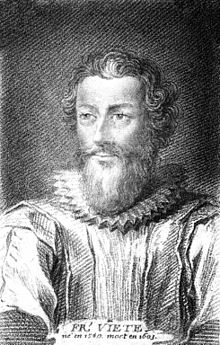
\includegraphics[height=4cm]{../../modules/history/pictures/francoisviete.jpg}

\hfil\hfil Fran\c{c}ois Vi\`ete(1540-1603)


\hfil\hfil Latinized: Franciscus Vieta

\hfil\hfil French mathematician

\hfil\hfil Known for: first symbolic algebra textbook
\end{frame}

\begin{frame}
\hfil\hfil $\begin{array}{rcll|l} ax^2+bx+c&\alertNoH{0}{=} &a\left( x- x_1\right) \left(x-x_2\right) \\~\\
\alertNoH{6}{x_1+x_2} &\alertNoH{6}{=} &\displaystyle \alertNoH{6}{-\frac{b}{a}} &&\text{Vieta's formulas}\\
\alertNoH{2}{x_1x_2}&\alertNoH{2}{=}&\displaystyle \alertNoH{2}{\frac{c}{a}}\\
\end{array}
$
\begin{example}
Factor the quadratic.
\[
x^2+5x+6 \uncover<2->{=(x+\fcAnswerUncover{2}{8}{2} )(x+\fcAnswerUncover{2}{8}{3})}
\]
\begin{itemize}
\item<2-> The product of the two roots: $\alertNoH{2,3,4,5}{x_1x_2=6}$.
\item<3-> The divisors of  $\alertNoH{3}{6}$ are $\alertNoH{3}{\alertNoH{4}{\pm 1},\alertNoH{5}{\pm 2}, \alertNoH{5}{\pm 3}, \alertNoH{4}{\pm 6}}$.
\item<4-> Therefore the pair $x_1, x_2$ is $\alertNoH{4}{\pm 1,\pm 6} $ or $\alertNoH{5}{\pm 2,\pm 3}$. 
\item<6-> The sum of the two roots: $\alertNoH{6}{x_1+x_2=-5}$ 
\end{itemize}
\end{example}
\end{frame}
\begin{frame}
\hfil\hfil $ax^2+bx+c=a\left( x- x_1\right)\left(x-x_2\right),\quad\quad\quad\quad \left|\begin{array}{rcl}
x_1x_2&=&\displaystyle \frac{c}{a}\\
x_1+x_2&=&\displaystyle-\frac{b}{a}
\end{array}\right.
$
\vskip -0.05cm
\begin{example}
Factor the quadratic.

\hfil\hfil$
x^2+3x+\alertNoH{2}{1} \uncover<2->{=\left(x\uncover<1-12>{+} \alertNoH{2}{ \fcAnswerUncover{2}{13}{-
\left(\frac{ -3 + \sqrt{5 }}{2}\right)
}} \right)
\left( x \uncover<1-12>{+} \alertNoH{2}{ \fcAnswerUncover{2 }{13}{
-\left(\frac{ -3 - \sqrt{5 }}{2}\right)
}}\right)}
$
\begin{itemize}
\item<2-> The product of the two roots: $\alertNoH{2,3}{x_1x_2=1}$.
\item<3-> Integer options: $\alertNoH{3,4}{ x_1=1, x_2=1}$ and $\alertNoH{3,5}{x_1=-1,x_2=-1}$.
\item<4-> $\begin{array}{rcl}
(x\alertNoH{4}{-1})(x\alertNoH{4}{-1})\uncover<6->{&=&(x-1)^2=x^2-2x+1}\\
(x+\alertNoH{5}{1})(x+\alertNoH{5}{1})\uncover<6->{&=&(x+1)^2=x^2+2x+1}
\end{array}$ \uncover<6->{both don't work.}
\item<7-> $\Rightarrow$ No easy factorization; must use quadratic formula.
$
\begin{array}{rcl}
\alertNoH{12,13}{x_1,x_2} &=&\displaystyle \frac{-\alertNoH{9}{ b}\pm \sqrt{{\alertNoH{9}{ b}}^2- 4{\alertNoH{8}{a} }\alertNoH{10 }{c}}}{2 {\alertNoH{8}{ a} }} \uncover<8->{ = \frac{- \alertNoH{9}{ 3} \pm \sqrt{\alertNoH{11}{ {\alertNoH{9}{3}}^2 -4 \cdot \alertNoH{8}{1 }\cdot \alertNoH{10}{1}}}}{ 2\cdot \alertNoH{8}{1}}}\\
\uncover<11->{&=&\displaystyle \alertNoH{12,13}{ \frac{ -3 \pm \sqrt{\alertNoH{11}{5 }}}{2}}}
\end{array}
$
\end{itemize}
\end{example}
\end{frame}
\section{Factorization overview}
\begin{frame}
Recall that $i^2=-1$, $\sqrt{-1}=i$.
\begin{example}[Polynomial factorizations]
$
\renewcommand{\arraystretch}{2}
\begin{array}{rcl}
\alertNoH{2,3}{2x^2+3x-5}&\alertNoH{2,3}{=}& \uncover<2->{ (\fcAnswer{3}{ \alertNoH{4 }{2}x +5})( \fcAnswer{3}{x -1}) \uncover<4->{= \alertNoH{4}{2} \left(x- \left(- \frac{5 }{ \alertNoH{4}{2} }\right)\right)(x-1)} }\\
\alertNoH{18}{x^2 \alertNoH{5}{+} 1} &\alertNoH{18}{=}& \uncover<5->{ x^2 \alertNoH{5}{-}(\alertNoH{6}{\alertNoH{5}{-}1} ) \uncover<6->{= {\alertNoH{7}{x}}^{\alertNoH{9}{2}} {\alertNoH{9}{-}} \alertNoH{6}{ {\alertNoH{8}{i}}^{\alertNoH{9}{2}}}} \uncover<7->{=\alertNoH{18}{ ({\alertNoH{7}{x}}{\alertNoH{9}{+}}{\alertNoH{8}{i}})({\alertNoH{7}{x}}{\alertNoH{9}{-}}{\alertNoH{8}{i}})}}} \\
\alertNoH{10}{{\alertNoH{11}{x}}^{\alertNoH{13}{4}} \alertNoH{13}{-} \alertNoH{12}{ 1}}&\alertNoH{10}{ =}&\uncover<10->{ \alertNoH{10}{ \alertNoH{14}{ ({ \alertNoH{11,15}{x }}^{ \alertNoH{13,17}{2} } \alertNoH{13,17}{-} \alertNoH{12,16}{ 1}) } ({\alertNoH{11}{x}}^{ \alertNoH{13}{2} } { \alertNoH{13}{+} } \alertNoH{12}{1 })}\uncover<14->{ =\alertNoH{14} {( \alertNoH{15}{x} \alertNoH{17}{-} \alertNoH{16}{ 1} )( \alertNoH{15}{x} \alertNoH{17}{+} \alertNoH{16}{ 1})} (\alertNoH{18}{ x^2+1} )} }\\
\uncover<18->{&\alertNoH{0}{ =} & (x-1)(x+1) \alertNoH{18}{(x-i)(x+i)}} \\
\alertNoH{19}{x^4+1}&\alertNoH{19}{=}&\uncover<19->{ \alertNoH{19}{ \left(\alertNoH{20}{ x^2- \sqrt{2}x+1} \right)\left( \alertNoH{21}{x^2+\sqrt{2}x+1} \right)}}\\
\uncover<20->{&\alertNoH{0}{=}&
\alertNoH{20}{
\left(x-\left(\frac{\sqrt{2}}{2}+\frac{\sqrt{2}}{2}i\right)\right)
\left(x-\left(\frac{\sqrt{2}}{2}-\frac{\sqrt{2}}{2}i\right)\right)
}
\\&&
\alertNoH{21}{
\left(x-\left(-\frac{\sqrt{2}}{2}+\frac{\sqrt{2}}{2}i\right)\right)
\left(x-\left(-\frac{\sqrt{2}}{2}-\frac{\sqrt{2}}{2}i\right)\right)
}
}
\end{array}$
\end{example}

 \end{frame}
\begin{frame}
\begin{theorem}[The Fundamental Theorem of Algebra]
For every polynomial we have the factorization
\[
p(x)=\alertNoH{4}{a_0} x^{\alertNoH{3}{n}}+a_1x^{n-1}+\dots + a_n=\alertNoH{2}{\alertNoH{4}{a_0} (x-\alertNoH{5}{x_1})\dots (x-\alertNoH{5}{x_n})},
\] 
where $x_1,\dots, x_n$ are the (not necessarily different) roots of $p(x)$. 
\end{theorem}
\begin{itemize}
\only<1-7>{
\item<2-> Every pol. of \alertNoH{3}{deg. $n$} can be factored as \alertNoH{2}{product of $n$ linear factors}.
}
\item<5-> \alertNoH{7,8}{ \alertNoH{5}{$x_1,\dots, x_n$ may be complex} numbers. Reminder: complex numbers are of the form $p+qi$, where $i^2=-1$ and $\sqrt{-1}=i$.}
\only<1-7>{
\item<6-7> While we can find $x_1, \dots$ with arbitrary precision, \alertNoH{6}{there may not be exist a formula involving radicals for computing each $x_1,\dots, x_n$}.
}
\end{itemize}
\uncover<9->{
\begin{Corollary}
Every real polynomial can be factored into a product of real linear terms and real quadratic terms with no real roots, i.e., factors of form 
\begin{itemize}
\item $(x-r)$, where $r$ is real and
\item $ax^2+bx+c$ with $b^2-4ac<0$ where $a,b,c$ are real.
\end{itemize}
\end{Corollary}
}

\vskip 10cm
\end{frame}
\begin{frame}
$\begin{array}{r@{}c@{}l}
a_0 x^{n}+a_1x^{n-1}+\dots + a_n&=& a_0 (x-x_1)\dots (x-x_n)\\
&=&\text{prod. real quadratics no roots \& lin. terms.}
\end{array}
$

\begin{example}

$
\renewcommand{\arraystretch}{2}
\begin{array}{@{\!\!}r@{}c@{}l@{}l@{}|l}
\alertNoH{2}{2x^2+3x-5}&\alertNoH{2}{=} &(2x+5)(x-1)= \alertNoH{2}{ 2\left(x- \alertNoH{3}{ \left(-\frac{5 }{2}\right)} \right)(x-\alertNoH{3}{1})} \uncover<2->{&&} \uncoverAlert{2}{ \alertNoH{3}{\text{real roots}}} \\
\alertNoH{4}{x^2+1}&\alertNoH{4}{=} &x^2-(-1)=x^2-i^2= \alertNoH{4}{(x-(\alertNoH{5}{-i}) )(x-\alertNoH{5}{i})} \uncover<4->{&&} \uncoverAlert{4}{\alertNoH{5}{ \text{complex roots}}} \\
\alertNoH{6}{x^4-1} &\alertNoH{6}{=}&(x^2-1)(x^2+1)=(x-1)(x+1)(x^2+1)\\
&\alertNoH{0}{=}& \alertNoH{6}{(x-\alertNoH{7}{1})(x-\alertNoH{7}{(-1)})(x-\alertNoH{7}{i})(x-(\alertNoH{7}{-i}))} \uncover<6->{&&} \uncoverAlert{6}{\alertNoH{7}{\text{mixed roots}}}\\
\alertNoH{8}{x^4+1}&\alertNoH{8}{=}&(x^2-\sqrt{2}x+1)(x^2+\sqrt{2}x+1)\\
&\alertNoH{0}{=}&
\alertNoH{8}{
\! \left(x-\alertNoH{9}{\left(\frac{\sqrt{2}}{2}+\frac{\sqrt{2}}{2}i\right)}\right)
\left(x-\alertNoH{9}{\left(\frac{\sqrt{2}}{2}-\frac{\sqrt{2}}{2}i\right)}\right)
}
\\&&
\alertNoH{8}{
\! \left(x-\alertNoH{9}{\left(-\frac{\sqrt{2}}{2}+\frac{\sqrt{2}}{2}i\right)}\right)\!\!
\left(x-\alertNoH{9}{\left(-\frac{\sqrt{2}}{2}-\frac{\sqrt{2}}{2}i\right)}\right)
}
\uncover<8->{&&} \uncoverAlert{8}{ \alertNoH{9}{\text{complex roots}}}
\end{array}$
\end{example}

 \end{frame}
\begin{frame}
\frametitle{Factoring polynomials in practice}
\begin{itemize}
\item In theory every polynomial can be factored.
\[a_0 x^{n}+a_1x^{n-1}+\dots + a_n=a_0 (x- \alertNoH{2}{x_1} )\dots (x-\alertNoH{2}{ x_n} )
\]
\item<2-> Theory guarantees numerical approximations for roots $\alertNoH{2}{ x_1,\dots, x_n} $. 
\item<3-> \alertNoH{3,4,6}{Can we find algebraic formulas} for $x_1, \dots, x_n$?
\item<4-> \alertNoH{4}{No}, if using finitely many operations $+,-,*,/,\sqrt[n]{~}$.
\item<5-> First (advanced) proof by Norwegian Niels Henrik Abel(1824) based on work of Italian Paolo Ruffini(1799). 
\item<6-> \footnotesize{ \alertNoH{6}{Yes}, with extra operations. Difficult: google Galois Theory to get started.}
\end{itemize}
\end{frame}

\begin{frame}
\frametitle{What does factorization mean?}
\begin{itemize}
\item Based on context, ``to factor a polynomial'' means one of:
\begin{itemize}
\item<2-> Factor the polynomial \alertNoH{3}{over the rational numbers}. Use integers/quotients, but no $\sqrt[n]{~}$).
\item<4-> Factor the polynomial \alertNoH{5}{over the real numbers}. Use radicals and/or numerical approximations, \alertNoH{5}{no use of $i=\sqrt{-1}$}.
\item<6-> Fully factor the polynomial \alertNoH{7}{using complex numbers}.
\end{itemize}
\end{itemize}
\begin{tabular}{|c|c|}\hline
These poly's are equal&Type of factorization\\\hline
 $\alertNoH{3}{x^4+1}$&\uncover<2->{ \alertNoH{3}{factored over rationals}}\\\hline
$\alertNoH{5}{(x^2-\sqrt{2}x+1)(x^2+\sqrt{2}x+1)}$&\uncover<4->{ \alertNoH{5}{factored over the reals}}\\\hline
$\begin{array}{r}
\alertNoH{7}{ \left(x-\left(\frac{\sqrt{2}}{2}+\frac{\sqrt{2}}{2}i\right)\right)
\left(x-\left(-\frac{\sqrt{2}}{2}+\frac{\sqrt{2}}{2}i\right)\right) }\\
\alertNoH{7}{ \left(x-\left(\frac{\sqrt{2}}{2}-\frac{\sqrt{2}}{2}i\right)\right)
\left(x-\left(-\frac{\sqrt{2}}{2}-\frac{\sqrt{2}}{2}i\right)\right)}
\end{array}$&\uncover<6->{ \alertNoH{7}{ full complex factorization}} \\\hline
\end{tabular}


\end{frame}
\begin{frame}
\frametitle{Factorization over the rationals}
\begin{itemize}
\item Suppose we want to factor a polynomial using only rational numbers (no $\sqrt[n]{~}$ or numerical approximations).
\item<2-> No guarantee to get:
\[
a_0 x^{n}+a_1x^{n-1}+\dots + a_n=a_0 (x- \alertNoH{2}{x_1} )\dots (x-\alertNoH{2}{ x_n} )
\]
\item<3-> A factorization using rationals may have arbitrarily large factors.
\item<4-> Efficient algorithms for factoring using rationals exist.
\begin{itemize}
\item<5-> Kronecker algorithm (German Leopold Kronecker (1823-1891)).
\item<6-> Methods based on finite fields.
\begin{itemize}
\item<7-> Cantor-Zassenhaus factorization algorithm.
\end{itemize}
\item<8-> Lenstra-Lenstra-Lov\'{a}sz algorithm. 
\end{itemize}
\item<9-> \alertNoH{9}{Above methods require computer}; \alertNoH{10}{no rational roots assumption}.
\item<10-> \alertNoH{10}{If we assume rational roots} there are practical algorithms \alertNoH{10}{by hand}.
\end{itemize}
\end{frame}

\begin{frame}
\frametitle{A few guiding examples}
Consider factoring the following using rationals:

\[
\begin{array}{l}
3 x^{2}+8x-11 \\\hline
x^{3}-6 x+4\\\hline
6 x^{3}-19 x^{2}+17 x-3\\
x^{4}-11 x^{2}+1\\\hline
2095632 x^{20}-3849552 x^{19}-3255849 x^{18}+4179303 x^{17}\\
-13505499 x^{16}+5980266 x^{15}+4196607 x^{14}-6906046 x^{13}\\
+29529137 x^{12}+7546174 x^{11}-4385895 x^{10}+26306731 x^{9}\\
+7651238 x^{8}-47703690 x^{7}+3048170 x^{6}\\
-20029315 x^{5}-25010625 x^{4}+4630400 x^{3}\\
-17212025 x^{2}+14818375 x+17892875
\end{array}
\]


\end{frame}


\section{Factorizations using formulas}
\begin{frame}
\begin{theorem}
The quadratic $ax^2+bx+c$ factors as follows.
\[
ax^2+bx+c=a(x-x_1)(x-x_2),
\]
where $x_1$ and $x_2$ are the roots of the quadratic, given by: 
\[
x_1, x_2=\frac{-b\pm \sqrt{b^2-4ac}}{2a}
\]
\end{theorem}
\end{frame}
\begin{frame}
\uncover<16->{$ ax^2+bx+c=\alertNoH{18}{a}\left( x- \alertNoH{19,35}{ x_1}\right) \left(x- \alertNoH{20,34}{x_2}\right)$\uncoverAlert{22}{, where $x_1, x_2 = \frac{-b \pm \sqrt{b^2-4ac}}{2a}$.}}
\begin{example}
Factor the polynomial. If possible, guess the factorization.

\hfil\hfil $\begin{array}{rcll|l}
\alertNoH{14,15}{\alertNoH{24}{3}x^2+\alertNoH{25}{8} x\alertNoH{26}{- 11}}\uncover<2->{ &=& (\uncover<3->{\alertNoH{16}{3} x+}  \fcAnswerUncover{2}{15}{11})(\uncover<3->{x} \uncover<3-14>{+} \fcAnswerUncover{2}{15}{-1})}\\
\uncover<16->{&=& \alertNoH{16,18}{3} \left(x \alertNoH{17}{-} \left(\alertNoH{19,35}{ \alertNoH{17}{-} \frac{11}{ \alertNoH{16}{3}}} \right) \right)(x- \alertNoH{20,34}{1}) }\\ 
\end{array}
$

\begin{itemize}
\only<handout:1|1-20>{%
\item<3-> If there is a factorization using integers, it should be of the form 

\hfil \hfil$
\begin{array}{rcl}
3 x^2+\alertNoH{10,12}{ 8}x \alertNoH{11,12}{-11} &\alertNoH{0}{=} &(\alertNoH{4,5}{3x} +\alertNoH{6,7,14,15}{p})(\alertNoH{4,6}{x}+ \alertNoH{5,7,14,15}{q})\\
\uncover<4->{& \alertNoH{0}{=} &\alertNoH{4}{3x^2}+ \alertNoH{5}{ \alertNoH{9}{3}\alertNoH{8}{ x} \alertNoH{9}{q}}+ \alertNoH{6}{ \alertNoH{9}{p}\alertNoH{8}{x}}+\alertNoH{7}{pq}}\\
\uncover<8->{&\alertNoH{0}{=} & 3x^2+\alertNoH{8}{x}( \alertNoH{9,10,12}{ 3q+p})+ \alertNoH{11,12}{ pq} }\\
\multicolumn{3}{c}{\uncoverAlert{12}{\text{(Vieta's formulas) }} \uncover<10->{\text{This means that  :}}}\\
\uncover<10->{\alertNoH{10,12,14}{8}&\alertNoH{12,14}{=}&\alertNoH{10,12,14}{3q +p}}\\
\uncover<10->{\alertNoH{11,12,13,14}{-11}&\alertNoH{12,13,14}{=}&\alertNoH{11,12,13,14}{pq}}\\
\multicolumn{3}{c}{\uncover<13->{\alertNoH{13}{p,q \text{ must be divisors of 11: }\pm 1,\pm 11 }}}\\
\uncover<14->{\alertNoH{14,15}{p}&\alertNoH{14,15}{=}& \fcAnswer{15}{11} } \\
\uncover<14->{\alertNoH{14,15}{q}&\alertNoH{14,15}{=}& \fcAnswer{15}{-1}} \\
\end{array}
$
}
\only<handout:2|21->{
\item<21-> What if we can't guess the factorization?
\item<22-> \alertNoH{22}{Use the formulas for $x_1, x_2$}.

\hfil \hfil$\renewcommand{\arraystretch}{2}
\begin{array}{rcl}
\alertNoH{22,34,35}{x_1, x_2} &=& \displaystyle \frac{-\alertNoH{24}{ b}\pm \sqrt{{ \alertNoH{24}{ b}}^2-4\alertNoH{23}{a}\alertNoH{25}{ c} }}{2\alertNoH{23}{ a}}
\uncover<23->{=\displaystyle \frac{-\alertNoH{24}{8}\pm \sqrt{{ \alertNoH{24}{8}}^2 \alertNoH{27}{-}  \alertNoH{26}{4}\cdot \alertNoH{23,26}{3} \cdot (\alertNoH{25}{\alertNoH{27}{-} \alertNoH{26}{11}})}}{\alertNoH{28}{ 2\cdot \alertNoH{23}{3}}}}\\
\uncover<26->{&=&\displaystyle \frac{-8 \pm \sqrt{\alertNoH{29}{ 64 \alertNoH{27}{+} \alertNoH{26}{132}}}}{\alertNoH{28}{6}} \uncover<29->{=\frac{-8 \pm  \alertNoH{30}{\sqrt{\alertNoH{29}{196 }} } }{6}}}\\
\uncover<30->{&=&\displaystyle \frac{-8 \pm\alertNoH{30}{ 14} }{6}\uncover<31->{= \left\{
\begin{array}{l}
\displaystyle \alertNoH{32}{\frac{-8+14 }{6}} \uncoverAlert{32}{ = \frac{6}{6}= \alertNoH{34}{1}} \\
\displaystyle \alertNoH{33}{\frac{-8-14 }{6}} \uncoverAlert{33}{ =-\frac{22}{6} =\alertNoH{35}{-\frac{11}{3}}}
\end{array}
\right. 
} } 
\end{array}
$
}
\end{itemize}

\end{example}

\vskip 10cm
\end{frame}
\begin{frame}
\frametitle{Cardano's formula}
\begin{theorem}[Cardano's formula for depressed monic cubic]
The equation 
\[
x^3+px+q=0
\]
has its roots given by:

\[
\begin{array}{rcl}
x_1 &=&\displaystyle  ~~~ \sqrt[3]{-\frac{q}{2}-\sqrt{\frac{q^2}{4}-\frac{p^3}{27}}}+~~~\sqrt[3]{-\frac{q}{2}+ \sqrt{\frac{q^2}{4}-\frac{p^3}{27}}}\\
x_2 &=&\displaystyle \omega  \sqrt[3]{-\frac{q}{2}-\sqrt{\frac{q^2}{4}-\frac{p^3}{27}}}+\omega^2 \sqrt[3]{-\frac{q}{2} + \sqrt{\frac{q^2}{4}-\frac{p^3}{27}}}\\
x_3 &=&\displaystyle  \omega^2 \sqrt[3]{-\frac{q}{2}-\sqrt{\frac{q^2}{4}-\frac{p^3}{27}}}+\omega \sqrt[3]{-\frac{q}{2}+\sqrt{\frac{q^2}{4}-\frac{p^3}{27}}}\\
\end{array}
\]
where $\omega =\displaystyle \frac{-1+i\sqrt{3}}{2} = \cos 120^\circ + i \sin 120^\circ$  (the third root of unity).
\end{theorem}	
\end{frame}
\begin{frame}
	\hfil\hfil 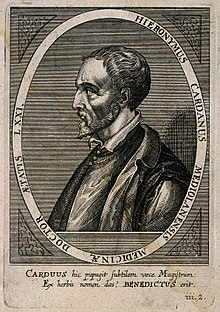
\includegraphics[height=4cm]{../../modules/history/pictures/cardano.jpg}
	
	\hfil\hfil Gerolamo Cardano (1501-1576)
	
	\hfil\hfil Italian mathematician
	
	\hfil\hfil Known for: Cardano's formula
	
	
\end{frame}




\begin{frame}
\frametitle{\alertNoH{11}{Should we use Cardano's formula to factor? \uncover<11->{No.}}}

\begin{example}
Try to factor $\begin{array}{rcl} 
x^{3} {\alertNoH{4}{-6}} x+{\alertNoH{5}{4}}\uncover<7->{ &=&(x-2)(x^{2}+2 x-2)}\\
\uncover<8->{&=&(\alertNoH{9}{x-2})\left(\alertNoH{9}{x-1+\sqrt{3}}\right)\left(\alertNoH{9}{x-1-\sqrt{3}}\right)}\end{array}$ using Cardano's formula.\uncover<2->{ \alertNoH{2}{By Fundamental Theorem of Algebra} $\Rightarrow$ can factor if we know \alertNoH{2}{roots}.} \uncover<3->{We know roots from \alertNoH{3}{Cardano's f-la}.}

$\begin{array}{@{}c@{}l}
\uncover<2->{=&\alertNoH{2}{ (x- \alertNoH{3}{x_1} )(x-x_2)(x-x_3)} }\\
\uncover<3->{=&\left(x- \alertNoH{3}{ \sqrt[3]{-\frac{{\alertNoH{5}{q}}}{2}-\sqrt{\frac{{\alertNoH{5}{q}}^2}{4}-\frac{{\alertNoH{4}{p}}^3}{27}}} - \sqrt[3]{-\frac{{\alertNoH{5}{q}}}{2}+ \sqrt{\frac{{\alertNoH{5}{q}}^2}{4} -\frac{{ \alertNoH{ 4}{p}}^3}{27}}}} \right)(x-x_2)(x-x_3)} \\
\uncover<4->{
=&\left(x-\alertNoH{6}{ \sqrt[3]{-\frac{{\alertNoH{5}{4}}}{2}-\sqrt{\frac{{\alertNoH{5}{4}}^2}{4}-\frac{{\alertNoH{4}{(-6)}}^3}{27}}} - \sqrt[3]{-\frac{{\alertNoH{5}{4}} }{2}+ \sqrt{\frac{{\alertNoH{5}{4}}^2}{4} -\frac{{\alertNoH{4}{(-6)}}^3}{27}}}} \right)(x-x_2)(x-x_3)}\\
\uncover<6->{
=&\left(\alertNoH{9}{ x-  \alertNoH{6,10}{ \sqrt[3]{-2\sqrt{-1}-2}- \sqrt[3]{2\sqrt{-1}-2}}} \right)(x-x_2)(x-x_3)
}
\end{array}
$

\uncover<10->{ Problem: $\alertNoH{10}{ \sqrt[3]{-2\sqrt{-1}-2}- \sqrt[3]{2\sqrt{-1}-2}}$ is not simplified (in fact, it equals $2$).}
\end{example}

\end{frame}
\section{Polynomial division}
\begin{frame}
\begin{example}[Polynomial long division]
Divide with quotient and remainder $\alertNoH{2}{ x^3+2x^2+1}$ by $\alertNoH{3}{x- 1}$.

\uncover<2->{

\renewcommand{\arraystretch}{1.2}\begin{longtable}{@{}c@{}c@{}c@{}c@{}c@{}c@{}c@{}c@{}c}\uncover<23->{\alertNoH{23}{\textbf{Quotient: }}}&\multicolumn{8}{c}{ \fcAnswer{5}{\alertNoH{6, 7, 23, 5}{$x^{2}$}} \uncover<11->{\alertNoH{12, 13, 23, 11}{$+$}} \fcAnswer{11}{\alertNoH{12, 13, 23, 11}{$3x $}} \uncover<17->{\alertNoH{18, 19, 23, 17}{$+$}} \fcAnswer{17}{\alertNoH{18, 19, 23, 17}{$3$}} }\\ \cline{2-9} \cline{2-9}\multicolumn{1}{c|}{ \alertNoH{3, 4, 5, 6, 7, 10, 11, 12, 13, 16, 17, 18, 19}{$x $} \alertNoH{3, 6, 7, 12, 13, 18, 19}{$-$} \alertNoH{3, 6, 7, 12, 13, 18, 19}{$1$} }&&\alertNoH{2, 4, 5, 8, 9}{$x^{3}$}&\alertNoH{2, 8, 9}{$+$}&\alertNoH{2, 8, 9}{$2x^{2}$}&&&\alertNoH{2, 8, 9}{$+$}&\alertNoH{2, 8, 9}{$1$}\\\uncover<6->{\uncover<8->{\alertNoH{8, 9}{$\overline{\phantom{A}}$}}&&\fcAnswer{7}{\alertNoH{8, 9, 7}{$x^{3}$}}&\uncover<7->{\alertNoH{8, 9, 7}{$-$}}&\fcAnswer{7}{\alertNoH{8, 9, 7}{$x^{2}$}}&&&\\\cline{2-9}}\uncover<8->{&&&&\fcAnswer{9}{\alertNoH{10, 11, 14, 15, 9}{$3x^{2}$}}&&&\uncover<9->{\alertNoH{14, 15, 9}{$+$}}&\fcAnswer{9}{\alertNoH{14, 15, 9}{$1$}}\\\uncover<12->{\uncover<14->{\alertNoH{14, 15}{$\overline{\phantom{A}}$}}&&&&\fcAnswer{13}{\alertNoH{14, 15, 13}{$3x^{2}$}}&\uncover<13->{\alertNoH{14, 15, 13}{$-$}}&\fcAnswer{13}{\alertNoH{14, 15, 13}{$3x $}}&\\\cline{4-9}}}\uncover<14->{&&&&&&\fcAnswer{15}{\alertNoH{16, 17, 20, 21, 15}{$3x $}}&\uncover<15->{\alertNoH{20, 21, 15}{$+$}}&\fcAnswer{15}{\alertNoH{20, 21, 15}{$1$}}\\\uncover<18->{\uncover<20->{\alertNoH{20, 21}{$\overline{\phantom{A}}$}}&&&&&&\fcAnswer{19}{\alertNoH{20, 21, 19}{$3x $}}&\uncover<19->{\alertNoH{20, 21, 19}{$-$}}&\fcAnswer{19}{\alertNoH{20, 21, 19}{$3$}}\\\cline{6-9}}}\uncover<20->{\uncover<24->{\textbf{\color{orange}Remainder: }}&&&&&&&&\fcAnswer{21}{\alertNoH{21}{{\only<22->{\color{orange}}$4$}}}\\}\end{longtable} $\vphantom{\frac{x^1}{x^1}}$\only<4,5>{Divide \alertNoH{4,5}{$x^{3}$ } by \alertNoH{4,5}{$x $}.}\only<6, 7>{Multiply \alertNoH{6, 7}{$x^{2}$} by divisor. }\only<8, 9>{Subtract last two polynomials.}\only<10,11>{Divide \alertNoH{10,11}{$3x^{2}$ } by \alertNoH{10,11}{$x $}.}\only<12, 13>{Multiply \alertNoH{12, 13}{$3x $} by divisor. }\only<14, 15>{Subtract last two polynomials.}\only<16,17>{Divide \alertNoH{16,17}{$3x $ } by \alertNoH{16,17}{$x $}.}\only<18, 19>{Multiply \alertNoH{18, 19}{$3$} by divisor. }\only<20, 21>{Subtract last two polynomials.}

}
\end{example}
\end{frame}
\section{Factorization using the Rational root theorem}
\begin{frame}\frametitle{Rational root theorem}
\begin{theorem}[Rational root theorem]
If a polynomial with rational coefficients $f(x)=a_0 x^n +a_1 x^{n-1}+\dots+a_{n-1}x+ a_n$ has rational root with reduced fraction $\frac{p}{q}$, then $p$ is a divisor of $a_n$ and $q$ is a divisor of $a_0$.
\end{theorem}
\uncover<2->{
\begin{proof}
Suppose $\frac{p}{q}$ is a root and so $
\begin{array}{rcll|l}
0=f\left(\frac{p}{q}\right) &=& a_0\left(\frac{p}{q}\right)^n + \dots +a_1\cdot \frac{p}{q} &&\text{mult. by }q^n \\
0&=& a_0 p^n + a_1  p^{n-1} q+ \dots + a_1 p q^{n-1} + a_0 q^n
\end{array}
$.

Since $0$ is divisible by $p$, so is the right hand side. All summands save the last one have a multiple of $p$, and so are divisible by $p$. It follows that the last summand $a_0 q^n$ is divisible by $p$. But $q$ is relatively prime to $p$, so $a_0$ must be divisible by $p$. The fact that $a_0$ is divisible by $q$ follows from a similar argument applied to the left-most summand.
\end{proof}
}
\end{frame}
\begin{frame}
\vskip -0.2cm
\begin{example}
Guess a rational root of $\alertNoH{6}{6} {\alertNoH{11}{x}}^{3}-19 {\alertNoH{11}{x}}^{2}+17 {\alertNoH{11}{x}} \alertNoH{4}{-3}$.

\uncover<2->{
By the rational root theorem, a rational root $\displaystyle \frac{\alertNoH{3, 4}{p }}{ \alertNoH{5,6}{ q}}$ has that 

\begin{itemize}
\item \alertNoH{3,4}{ $p$ is \alertNoH{7}{a divisor of $\fcAnswer{4}{-3}$},}\uncover<7->{ so $p$ is one of: $\alertNoH{7}{\pm 1, \pm 3}$.}
\item \alertNoH{5,6}{ $q$ is \alertNoH{8}{a divisor of $\fcAnswer{6}{6}$},}\uncover<8->{ so $q$ is one of: $\alertNoH{8}{\pm 1, \pm 2, \pm 3, \pm 6}$.}
\end{itemize}
}
\uncover<9->{ Therefore $\frac{p}{q}$ is one of $12$ possibilities: $\pm 1, \pm \frac{1}{3}, \pm \frac{1}{2}, \pm \frac{1}{6}, \pm 3, \pm \frac{3}{2}$. Try all:
}

\uncover<10->{
$
\begin{array}{rclcl}
f(1)&=& 6\cdot{\alertNoH{11} {1}}^3-19\cdot {\alertNoH{11} {1}}^2+17\cdot {\alertNoH{11} {1}}-3&=&1 \\
\uncover<12->{
f(-1)&=&6 \left(-1\right)^{3}-19 \left(-1\right)^{2}+17 \left(-1\right)-3&=&-45\\
f{}\left(3\right)&=&6\cdot 3^{3}-19\cdot 3^{2}+17\cdot 3-3&=&39\\
f{}\left(-3\right)&=&6 \left(-3\right)^{3}-19 \left(-3\right)^{2}+17 \left(-3\right)-3&=&-387\\
f{}\left(\frac{1}{3}\right)&=&6 \left(\frac{1}{3}\right)^{3}-19 \left(\frac{1}{3}\right)^{2}+17\cdot \frac{1}{3}-3&=&\frac{7}{9}\\
\vdots \\ 
f{}\left(\alertNoH{13}{\frac{3}{2}}\right)&=&6 \left(\frac{3}{2}\right)^{3}-19 \left(\frac{3}{2}\right)^{2}+17\cdot \frac{3}{2}-3&=&\alertNoH{13}{0}\\
}
\end{array}$

\uncover<13->{Answer: $\alertNoH{13}{x=\frac{3}{2}}$ is the only rational root.}
}


\end{example}
\end{frame}
\begin{frame}
Example: $\alertNoH{1}{6}x^3-19x^2+17x\alertNoH{1}{-3}$.
\begin{itemize}
\item Guessing rational roots: had to factor constant term, leading coefficient.
\item<2-> We wrote down all possibilities:
\begin{itemize}
\item<3-> Even on small example we get many possibilities!
\end{itemize}
\item<4-> An optimization: use numerical methods (say: Newton's method) to find floating point approximation for the root.
\item<5-> Say, we found $r=1.499$.
\item<6-> If root is rational, then its leading coefficient $6$ times $r$ is integer.
\item<7-> So: $1.499\cdot 6=8.994$. 

\item<8-> Round $8.944$ to nearest integer: $9$. 
\item<9-> Divide $9$ back by $6$ to get $\frac{3}{2}$. 
\item<10-> Now $\frac{3}{2}$: rational number close $r$.
\item<11-> In our algebra method, start with $\frac{3}{2}$ as our first guess. 
\end{itemize}
\end{frame}
\begin{frame}
\hfil\hfil 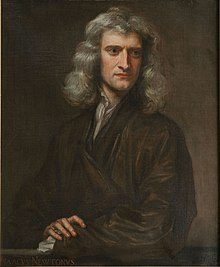
\includegraphics[height=4cm]{../../modules/history/pictures/newton.jpg}

\hfil\hfil Sir Isaac Newton (1642-1726)

\hfil\hfil English mathematician, physicist, natural philosopher

\hfil\hfil Known for: Calculus

\hfil\hfil Considered one of greatest scientists in history

\end{frame}
\begin{frame}
\vskip -0.1cm
\begin{example}
Demonstrate that $6 x^{3}-19 x^{2}+17 x-3$ is divisible by $(2x-3)$ using polynomial long division. \alertNoH{25,33}{Use your work to factor the cubic.} \alertNoH{34}{Solve the equation $6 x^{3}-19 x^{2}+17 x-3=0$}.

\vskip -0.2cm
\only<1-25| handout:1>
{\renewcommand{\arraystretch}{1.2}\begin{longtable}{@{}c@{}c@{}c@{}c@{}c@{}c@{}c@{}c@{}c}\uncover<23->{\alertNoH{23}{\textbf{Quotient: }}}&\multicolumn{8}{c}{ \fcAnswer{5}{\alertNoH{6, 7, 23, 5}{$3x^{2}$}} \uncover<11->{\alertNoH{12, 13, 23, 11}{$-$}} \fcAnswer{11}{\alertNoH{12, 13, 23, 11}{$5x $}} \uncover<17->{\alertNoH{18, 19, 23, 17}{$+$}} \fcAnswer{17}{\alertNoH{18, 19, 23, 17}{$1$}} }\\ \cline{2-9} \cline{2-9}\multicolumn{1}{c|}{ \alertNoH{3, 4, 5, 6, 7, 10, 11, 12, 13, 16, 17, 18, 19}{$2x $} \alertNoH{3, 6, 7, 12, 13, 18, 19}{$-$} \alertNoH{3, 6, 7, 12, 13, 18, 19}{$3$} }&&\alertNoH{2, 4, 5, 8, 9}{$6x^{3}$}&\alertNoH{2, 8, 9}{$-$}&\alertNoH{2, 8, 9}{$19x^{2}$}&\alertNoH{2, 8, 9}{$+$}&\alertNoH{2, 8, 9}{$17x $}&\alertNoH{2, 8, 9}{$-$}&\alertNoH{2, 8, 9}{$3$}\\\uncover<6->{\uncover<8->{\alertNoH{8, 9}{$\overline{\phantom{A}}$}}&&\fcAnswer{7}{\alertNoH{8, 9, 7}{$6x^{3}$}}&\uncover<7->{\alertNoH{8, 9, 7}{$-$}}&\fcAnswer{7}{\alertNoH{8, 9, 7}{$9x^{2}$}}&&&\\\cline{2-9}}\uncover<8->{&&&\uncover<9->{\alertNoH{10, 11, 14, 15, 9}{$-$}}&\fcAnswer{9}{\alertNoH{10, 11, 14, 15, 9}{$10x^{2}$}}&\uncover<9->{\alertNoH{14, 15, 9}{$+$}}&\fcAnswer{9}{\alertNoH{14, 15, 9}{$17x $}}&\uncover<9->{\alertNoH{14, 15, 9}{$-$}}&\fcAnswer{9}{\alertNoH{14, 15, 9}{$3$}}\\\uncover<12->{\uncover<14->{\alertNoH{14, 15}{$\overline{\phantom{A}}$}}&&&\uncover<13->{\alertNoH{14, 15, 13}{$-$}}&\fcAnswer{13}{\alertNoH{14, 15, 13}{$10x^{2}$}}&\uncover<13->{\alertNoH{14, 15, 13}{$+$}}&\fcAnswer{13}{\alertNoH{14, 15, 13}{$15x $}}&\\\cline{4-9}}}\uncover<14->{&&&&&&\fcAnswer{15}{\alertNoH{16, 17, 20, 21, 15}{$2x $}}&\uncover<15->{\alertNoH{20, 21, 15}{$-$}}&\fcAnswer{15}{\alertNoH{20, 21, 15}{$3$}}\\\uncover<18->{\uncover<20->{\alertNoH{20, 21}{$\overline{\phantom{A}}$}}&&&&&&\fcAnswer{19}{\alertNoH{20, 21, 19}{$2x $}}&\uncover<19->{\alertNoH{20, 21, 19}{$-$}}&\fcAnswer{19}{\alertNoH{20, 21, 19}{$3$}}\\\cline{6-9}}}\uncover<20->{\uncover<24->{\textbf{\color{orange}Remainder: }}&&&&&&&&$ { \only<22->{\color{orange}}\fcAnswer{21}{0}}$}\end{longtable} $\vphantom{\frac{x^1}{x^1}}$\only<4,5|handout:0>{Divide \alertNoH{4,5}{$6x^{3}$ } by \alertNoH{4,5}{$2x $}.}\only<6, 7| handout:0>{Multiply \alertNoH{6, 7}{$3x^{2}$} by divisor. }\only<8, 9| handout:0>{Subtract last two polynomials.}\only<10,11| handout:0>{Divide \alertNoH{10,11}{$-10x^{2}$ } by \alertNoH{10,11}{$2x $}.}\only<12, 13| handout:0>{Multiply \alertNoH{12, 13}{$-5x $} by divisor. }\only<14, 15| handout:0>{Subtract last two polynomials.}\only<16,17| handout:0>{Divide \alertNoH{16,17}{$2x $ } by \alertNoH{16,17}{$2x $}.}\only<18, 19| handout:0>{Multiply \alertNoH{18, 19}{$1$} by divisor. }\only<20, 21| handout:0>{Subtract last two polynomials.}}\uncover<23->{
$\begin{array}{@{}r@{}c@{}l}
\uncover<1-25| handout:1>{\textbf{(Divident)}&\alertNoH{0}{=}&  \textbf{(\alertNoH{23}{Quotient})} \cdot \textbf{(Divisor)}+ \textbf{(\alertNoH{24}{Remainder})}}\\
\alertNoH{25,26,33,35}{( 6x^3-19x^2+17x-3)}&\alertNoH{25,26}{=}&\alertNoH{25,26}{ (\alertNoH{23}{\alertNoH{29}{3}x^2\alertNoH{30}{-5} x+\alertNoH{31}{1} }) \cdot(2x-3)}\\
\only<26-|handout:2>{\uncover<27->{&\alertNoH{0}{=}&\alertNoH{33,35}{ \left(x- \fcAnswerUncover{27}{32}{\left(\frac{5+ \sqrt{13}}{6}\right)} \right)\left(x- \fcAnswerUncover{27}{32}{\left(\frac{5- \sqrt{13}}{6}\right)}\right)(2x-3)} }}
\end{array}
$
\only<26-|handout:2>{
\uncover<27->{
No easy factorization of quadratic, so use formula:

\hfil\hfil$
\alertNoH{32}{x_1,x_2}=\fcAnswer{28}{\frac{-b\pm\sqrt{b^2-4ac}}{2a}}\uncover<29->{=\frac{-(\alertNoH{30}{-5})\pm\sqrt{(\alertNoH{30}{-5})^2-4\cdot \alertNoH{29}{ 3}\cdot \alertNoH{31}{1} } }{2\cdot\alertNoH{29}{ 3} }}\uncoverAlert{32}{ =\frac{ 5\pm\sqrt{13}}{6}}
$
\uncover<34->{
We are ready to solve the equation.

\hfil\hfil $\begin{array}{rcl}
\alertNoH{34}{ 6x^3-19x^2+17x-3}&=&0\\
\uncover<35->{\alertNoH{35}{\left(\alertNoH{37}{ x- \left(\frac{5+ \sqrt{13} }{6} \right)}\right)\left(\alertNoH{38}{x- \left(\frac{5- \sqrt{13} }{6}\right)} \right) (\alertNoH{36}{2x-3})} &=&0}\\
\end{array}
$
}

\uncover<36->{
$\begin{array}{rclcrclcrcl}
\alertNoH{36}{\alertNoH{40}{2}x\alertNoH{39}{-3}}&\alertNoH{36}{=}&\alertNoH{36}{0}&\quad \alertNoH{41}{\textbf{or}} \quad &\alertNoH{37,41}{x}&\alertNoH{37,41}{=}& \alertNoH{37,41}{\left(\frac{5+ \sqrt{13}}{6}\right)}&\quad \alertNoH{41}{ \textbf{or} } \quad &\alertNoH{38, 41}{x} &\alertNoH{38, 41}{=} & \alertNoH{38, 41}{ \left(\frac{5- \sqrt{13}}{6}\right)} \\
\uncover<39->{ \alertNoH{41}{x}&\alertNoH{41}{=}&\alertNoH{41}{ \frac{ \alertNoH{39 }{3}}{ \alertNoH{40}{2}}}}
\end{array}
$
}
}
}
}

\end{example}
\vskip 10cm
\end{frame}


\begin{frame}
\begin{itemize}
\item Consider $f(x)=x^{4}-11 x^{2}+1$. 
\item<2-> If it has rational roots, then they must be $\pm 1$ by the rational root theorem, but $f(-1)=f(1)=-9$. So the polynomial has no rational roots. 
\item<3-> We need a general method to factor $f$.
\item<4-> One such method is the Kronecker algorithm.
\end{itemize}

\end{frame}
\begin{frame}
\hfil\hfil 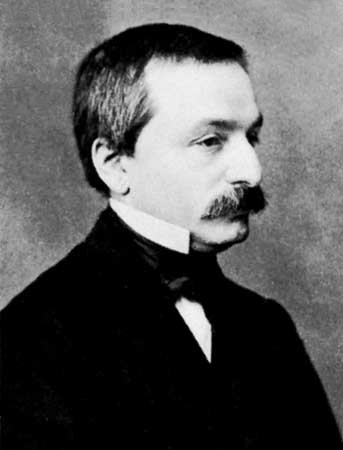
\includegraphics[height=4cm]{../../modules/history/pictures/kronecker.jpg}

\hfil\hfil Leopold Kronecker (1823 - 1891)

\hfil\hfil German mathematician

\hfil\hfil Known for: research in number theory and algebra


\end{frame}
\begin{frame}
\begin{theorem}[Gauss lemma]
Let $p(x)$ be a polynomial with integer coefficients and let 
\[
p(x)=q(x)\cdot r(x)
\] be a factorization so that $q$ and $r$ have rational coefficients. Then $q(x)$ and $r(x)$ can be re-scaled with multiplication by a constant to 
\[
\begin{array}{rcl}
\bar q(x) &=& c\cdot q(x)\\ 
\bar r(x) &=& \frac{1}{c} \cdot r(x)\\
p&=&\bar r(x)\bar q(x)
\end{array}
\] so that both $\bar q(x),\bar r(x)$ have integer coefficients.
\end{theorem}
\end{frame}
\begin{frame}
\hfil\hfil 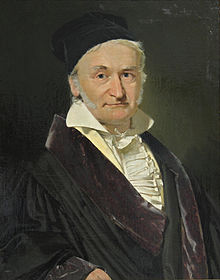
\includegraphics[height=4cm]{../../modules/history/pictures/gauss.jpg}

\hfil\hfil Johann Carl Friedrich Gauss (1777 - 1855)

\hfil\hfil German mathematician

\hfil\hfil Known for: Gaussian elimination

\hfil\hfil Considered one of the greatest mathematicians of all time


\end{frame}
\begin{frame}
\frametitle{A polynomial lemma}
Suppose we a polynomial $f(x)$ is prescribed $n+1$ values at $n+1$ distinct points: $f(x_0)=y_0, \dots, f(x_n)=y_n$.
\begin{lemma}[Lagrange interpolation]
There exists a unique polynomial $f(x)$ of degree $n$ with the values prescribed in $n+1$ distinct points.
\end{lemma}
\only<1-2>{
\uncover<2->{
\begin{proof}[Uniqueness]
Suppose we have two such polynomials: $f(x)$ and $\bar f(x)$. Then $h(x)=f(x)-\bar f(x)$ is a polynomial of degree $n$. We have that $h(x_0) = f(x_0)-\bar f(x_0)=0, \dots, h(x_n)= f(x_n)-\bar f(x_n)=0$, and so h vanishes at $n+1$ points. However, by the fundamental theorem of algebra, a non-zero polynomial of degree $n$ vanishes at at most $n$ points. Therefore $h(x)$ must be the zero polynomial, or $f(x)=\bar f(x)$, which establishes the uniqueness.
\end{proof}
}
}
\only<3->{
\begin{proof}[Existence]
Let $L_j(x)$ be the $j^{th}$ Lagrange polynomial:

\[L_j(x) = \frac{ (x-x_0)\dots \widehat{(x-x_j)} \dots (x-x_n) }{(x_j-x_0)\dots \widehat{(x_j-x_j)} \dots (x_j-x_n) },
\]

where the hat symbol indicates that the term is to be skipped. Then $L_j(x_j) = 1 $ and $L_j(x_i)=0$ for $i\neq j$. Therefore $f(x)=\sum_{j=0}^n y_j\cdot L_j(x)$ is the desired $n^{th}$-degree polynomial.

\end{proof}
}
\vskip 5cm
\end{frame}
\begin{frame}
	\hfil\hfil 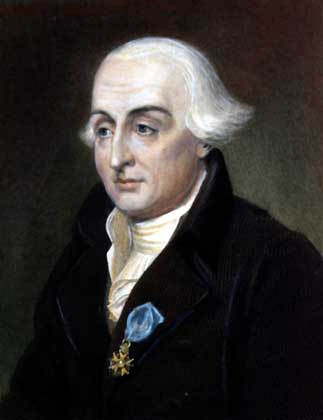
\includegraphics[height=4cm]{../../modules/history/pictures/lagrange.jpg}
	
	\hfil\hfil Joseph-Louis Lagrange (1736 - 1813)
	
	\hfil\hfil Italian mathematician, astronomer
	
	\hfil\hfil Known for: work on real analysis, mechanics, celestial mechanics
	
	
\end{frame}
\begin{frame}
\frametitle{Kronecker's method for polynomial factorization}
\begin{itemize}
\item Suppose $f(x)=p(x)q(x)$: factorization over the rationals.
\item<2-> Multiply by a rational constant so that $f(x)$ has integer coefficients.
\item<3-> Gauss lemma: $p(x), q(x)$ can be chosen with integer coefficients.
\item<4-> Let $p(x)$ be the smaller-degree divisor of degree $k$, $k\leq \frac{n}{2} $.
\item<5-> If we know $p(x)$ in $k+1$ points, we can reconstruct it.
\item<6-> Since $f(a)=p(a)q(a)$ so if $a$ is an integer $p(a)$ divides $f(a)$.

\item<7-> Pick the smallest $k+1$ integers: $0, \pm 1, \pm 2, \dots$.
\item<8-> Evaluate $f(x)$ at each of them: $f(0), f(\pm 1), f(\pm 2),\dots$.
\item<9-> Factor each of the numbers above and enumerate all possible divisors of $f(0)$, $f(\pm 1)$, $f(\pm 2)$ \dots. 
\item<10-> $\Rightarrow$ finitely many possibilities for factors $p(0), p(\pm 1), p(\pm 2), \dots $. 
\item<11-> Reconstruct all possible $p(x)$'s with Lagrange interpolation.
\item<12-> Try all candidates with polynomial division. 
\item<13-> If no candidate works, $f(x)$ cannot be factored over the rationals.
\end{itemize}
\end{frame}

\begin{frame}
\begin{example}
Use the Kronecker method to factor the polynomial: $f(x)=x^4-11x^2+1$. 
\only<1-11>{
\begin{itemize}
\item<2-> By Rational Root theorem, only possible rational roots are $\pm 1$ and none of them work.
\item<3-> $\Rightarrow$ we need to look for a $\deg 2$ factor $p(x)$. 
\item<4-> $\Rightarrow$ We need to know the value of $p(x)$ at $3$ points.
\item<5-> Evaluate $f(x)$ at $3$ points:
$\begin{array}{rclcl}
f(0)&=&0^4-11\cdot 0^2+1&=&1\\
f(1)&=&1^4-11\cdot 1^2+1&=&-9\\
f(-1)&=&(-1)^4-11\cdot (-1)^2+1&=&-9\\
\end{array}
$
\end{itemize}
\uncover<6->{
The possible divisors of $f(0)$ are $\alertNoH{6}{\pm 1}$, and of $f(-1), f(1)$: $\alertNoH{6}{\pm 1, \pm 3, \pm 9}$\uncover<7->{, for a total of $\alertNoH{7}{2\cdot 6\cdot 6=72}$ different possibilities.}} \uncover<8->{Suppose we try the divisors $p(0) = \alertNoH{9}{1}, p(1)=\alertNoH{9}{3}, p(-1)=\alertNoH{9}{-3}$.} 
}


\uncover<9->{ 
$
\alertNoH{11,12}{p(x)} = \alertNoH{10}{ \alertNoH{9}{1}\cdot \frac{(x-1)(x+1)}{(0-1)(0+1)} + \alertNoH{9}{3}\cdot \frac{x(x+1)}{1\cdot (1+1)} \alertNoH{9}{-3}\cdot \frac{x(x-1)}{-1\cdot(-1-1)}} \uncover<10->{=\alertNoH{10,11,12}{-x^{2}+3 x+1}}.
$
}

\only<12->{
\uncover<13->{
\footnotesize
Divide $\alertNoH{13}{x^4-11x^2+1}$ by $\alertNoH{13}{-x^{2}+3 x+1}$: 
\renewcommand{\arraystretch}{1.2}\begin{longtable}{|cccccc|} \hline\textbf{Divisor} &\multicolumn{5}{|c|}{\textbf{Quotient(s)}}\\$\alertNoH{13}{-x^{2}+3x +1}$& \multicolumn{5}{|l|}{$\alertNoH{13}{-x^{2}-3x +1}$}\\\hline$\underline{~}$&$\alertNoH{13}{x^{4}}$ & &$\alertNoH{13}{-11x^{2}}$ & &$\alertNoH{13}{+1}$ \\ &$x^{4}$ & $-3x^{3}$ & $-x^{2}$ & &\\\cline{2-6}$\underline{~}$&&$3x^{3}$ & $-10x^{2}$ & &$+1$ \\ &&$3x^{3}$ & $-9x^{2}$ & $-3x $ & \\\cline{2-6}$\underline{~}$&&&$-x^{2}$ & $+3x $ & $+1$ \\ &&&$-x^{2}$ & $+3x $ & $+1$ \\\cline{2-6}&&&&& \alertNoH{13}{0}\\ \hline\end{longtable}
}
\vskip -0.2cm

\uncover<14->{
\normalsize
Therefore $x^4-11x^2+1=\left(-x^2+3x+1\right)\left(-x^2-3x+1\right)=\left(x^2-3x-1\right)\left(x^2+3x-1\right)$
is the desired factorization.
}
}
\end{example}
\end{frame}
\begin{frame}
Factor the following example.
\[\begin{array}{l}
2095632 x^{20}-3849552 x^{19}-3255849 x^{18}+4179303 x^{17}\\
-13505499 x^{16}+5980266 x^{15}+4196607 x^{14}-6906046 x^{13}\\
+29529137 x^{12}+7546174 x^{11}-4385895 x^{10}+26306731 x^{9}\\
+7651238 x^{8}-47703690 x^{7}+3048170 x^{6}\\
-20029315 x^{5}-25010625 x^{4}+4630400 x^{3}\\
-17212025 x^{2}+14818375 x+17892875
\end{array}
\]
\begin{itemize}
\item If we run the Kronecker method on this, we get a total of $96370911975272721485253731942400\approx 9.6\cdot 10^{31}$ possibilities for the divisors of the polynomial.
\item $\Rightarrow$ we need a better method.
\end{itemize}

\end{frame}

\section{Connection between factorization with integers and modular one} 
\begin{frame}
\frametitle{Review of modular arithmetic $\left(\mathbb Z/n \mathbb Z\right)$}
\begin{definition}[Modular arithmetic notation]
Let $\alertNoH{3}{n\geq 0}$. If \alertNoH{2}{$a,b$ have same remainder} \alertNoH{3}{when divided by $n$}, we say that:

\hfil\hfil$
 a\alertNoH{2}{\equiv} b \alertNoH{3}{\mod n}
$
\end{definition}
\uncover<4->{Every number is equivalent $\mod n$ to one lying between $0$ and $n-1$:
\begin{example}
$\begin{array}{@{}r@{~}c@{~}l@{}ll|l}
\alertNoH{4,5,6}{10} &\alertNoH{4,5}{{\equiv}}& \fcAnswer{5}{\alertNoH{7}{3}} &\alertNoH{4,5,8}{\mod  7} &&\uncover<5->{\text{$\alertNoH{6}{ 10= \alertNoH{8}{7}\cdot 1 + \alertNoH{7}{3}}$  has \alertNoH{7}{remainder $3$} when \alertNoH{8}{div. by $7$}.}}\\
\uncover<9->{\alertNoH{9,10,11}{15} &\alertNoH{9,10}{{\equiv}}&\fcAnswer{10}{\alertNoH{12}{0}} &\alertNoH{9,10,13}{ \mod 5}&} &\uncover<10->{\text{$ \alertNoH{11}{15= 3\cdot \alertNoH{13}{ 5} +\alertNoH{12}{0} }$ has \alertNoH{12}{remainder $0$} when \alertNoH{13}{div. by $5$}.}}\\
\uncover<14->{\alertNoH{14,15,16}{-2} &\alertNoH{14,15}{{\equiv}}& \fcAnswer{15}{\alertNoH{17}{1}}& \alertNoH{14,15,18}{\mod 3}& } &\uncover<15->{\text{$\alertNoH{16}{-2 = \alertNoH{18}{3}\cdot (-1) + \alertNoH{17}{1}}$ has \alertNoH{17}{remainder $1$} when \alertNoH{18}{div. by $3$}}}
\end{array}
$
\end{example}
}
\uncover<19->{
Finding the number between $0 $ and $n-1$ as described above is called ``reducing a number modulo $n$''.
}
\end{frame}

\begin{frame}
\vskip -0.17cm
\begin{lemma}
Let $a_1 \equiv a_2 \mod n$ and $b_1\equiv b_2 \mod n$. 
\begin{itemize}
\item $a_1\pm b_1 \equiv a_2 \pm b_2 \mod n$\hfill (Mod. arithm. respects addition).
\item $a_1\cdot b_1 \equiv a_2 \cdot b_2 \mod n$\hfill  (Mod. arithm. respects multiplication).
\end{itemize}
\end{lemma}
\vskip -0.17cm
\begin{proof}[Proof. {[Multiplication respected]}]
Since $a_1 \equiv a_2  \mod n$ $\Rightarrow$ $a_1 = n\cdot p + a_2 $ for some $p$.

Since $b_1 \equiv b_2  \mod n$ $\Rightarrow$ $b_1 = n\cdot q + b_2 $ for some $q$.	

\hfil\hfil  $\begin{array}{rclll}
a_1 \cdot b_1 &=& ( n\cdot p + a_2)\cdot (n\cdot q + b_2 ) \\
&=& n^2 (p+q) + n(b_2+a_2) + b_2 + a_2 \\
&\equiv& b_2 + a_2\mod n
\end{array}
$
\end{proof}

\vskip -0.17cm
\uncover<2->{\begin{example}
Reduce $2030\cdot 201800003 \mod 2018$.

$\begin{array}{r@{~}c@{~}ll}
2030 &=& 2018+12 \equiv 12 &\mod 2018\\  
201800003 &=& 20180000+3 = 2018\cdot 10^4+3 \equiv 3 &\mod 2018\\  
2030\cdot 201800003&\equiv & 12\cdot 3= 36 &\mod 2018\\
\end{array}
$
\end{example}
}
\end{frame}
\begin{frame}
\frametitle{Notation for modular arithmetics}
\begin{itemize}
\item Recall
\[
4\equiv 11 \mod 7
\]
means $4$ and $11$ have same remainder when divided by $7$.
\item $\equiv$ respects all arithmetic operations.
\item We need to write $\mod n$ and $\equiv$ everywhere.
\item Can we use $=$ instead, and omit the $\mod n$?
\item Yes. 
\begin{definition}[Integers modulo $n$]
\[
\mathbb Z/n\mathbb Z \qquad \text{ or alternatively } \qquad \mathbb Z_n
\]
are called the integers modulo $n$.
\end{definition}
\item When reading $\mathbb Z/n\mathbb Z_n$: do not omit the ``modulo $n$'' part.
\item The notation $\mathbb Z/n\mathbb Z_n$ is less ambiguous, but $\mathbb Z_n$ is easier to read.
\item We use $\mathbb Z_n$ to conserve horizontal space. 
\end{itemize}

\end{frame}

\begin{frame}
\frametitle{$=$ vs $\equiv$}

\begin{itemize}
\item $\equiv$ stands for equivalence $\mod n$. We write $8\equiv 2 \mod 3 $.
\item We also have $(8\mod 3)= (2\mod 3)$: no need for $\equiv$ here.
\item Writing $\mod 3$ everywhere is cumbersome.
\item Convention: drop $\mod 3$, except for the last line:
\[
\begin{array}{c}
2+2+2+2 = 8=2 \mod 3\\
\text{instead of}\\

((2+2+2+2) (\mod 3))=(8 \mod 3) = (2\mod 3) \\
\end{array}
\]
\item We can write:
\[
2+2+2+2=8\equiv 2 \mod 3
\]
to stress the fact that $8\neq 2$ over $\mathbb Z$.
\item With variables, we can't always tell $=$ from $\equiv$:
\[
2+2+2+2=8 \mod p
\] 
\item Informally, we allow ourselves to write $8\in \mathbb Z_3$, where it's implied $8=2\mod 3$ are two different ways of writing $2\in \mathbb Z_3$.
\end{itemize}
\end{frame}
\begin{frame}
\begin{definition}A polynomial $p$ is called monic if its leading coefficient is $1$.
\end{definition}

\begin{example}
\begin{itemize}
\item $x^2+1$ is monic.
\item $-x^2+1$ is not.
\item $2x$ is not.

\item $(x^2+1) \mod 3$ is monic.
\item $(2x^2+1) \mod 3$ is not.
\item $4x^2+1 = (x^2+1) \mod 3$ is monic.
\end{itemize}
\end{example}
\end{frame}
\begin{frame}
\frametitle{B\'ezout's lemma}
\begin{lemma}[B\'ezout]
Suppose the greatest common divisor of $a$ and $b$ is $d$, where $a,b,d$ are integers or polynomials. Then there exist $r,s$ such that:
\[
ra+sb=d
\]
\end{lemma}
\end{frame}


\begin{frame}
	\vskip -0.2cm
	\footnotesize
\begin{lemma}[B\'ezout's lemma]
Let $a,b\in \mathbb  K[x]$ be non-constant monic polynomials with greatest common divisor $d$ with $\mathbb K$ - field (can be $\mathbb Q, \mathbb R, \mathbb Z_p$). $\Rightarrow$ there exist monic polynomials $r,s\in  \mathbb K[x]$ such that 
\[
ra+sb=d
\]
Furthermore $\deg r < \deg b$ and $\deg s < \deg a$.
\end{lemma}
\begin{proof}
\tiny 
\only<1|handout:1>{
Carry out the consecutive divisions with remainder


\hfil\hfil$
\begin{array}{rcll|l|lcl}
a&=& q_1b &+c_3 &\deg c_3 < \deg b &c_{n+1}|b, c_{n+1}|c_3&\Rightarrow& c_{n+1} | a\\
b&=& q_2c_3 &+c_4& \deg c_4 < \deg c_3& c_{n+1}|c_4, c_{n+1}|c_3&\Rightarrow& c_{n+1} | b \\
c_3&=&q_3 c_4&+c_5& \deg c_5 < \deg c_4& c_{n+1}|c_4, c_{n+1}|c_3&\Rightarrow& c_{n+1} | c_3 \\
&\vdots&&&&\vdots \\
c_{n-1}&=&q_{n-1} c_{n}&+c_{n+1}  & \deg c_{n+1} < \deg c_n& c_{n+1}|c_n, c_{n+1}|c_{n+1}&\Rightarrow& c_{n+1}|c_{n-1}\\
c_n&=&q_n c_{n+1}&+0  & \deg c_k \text{ decreases so we must reach }0& c_{n+1}|c_n
\end{array}
$

By reading the equations above in reverse order, we see that $c_{n+1}|c_n, c_{n+1}|c_{n-1}, \dots$ and so $c_{n+1}|a$ and $c_{n+1}|b$, i.e., $c_{n+1}$ is a common divisor of $a,b$. Transfer each term $q_{k-1}c_k $ to the left hand side and solve for $c_{n+1}$ as shown below:

\hfil\hfil$
\begin{array}{rrcl|lcr}
a&- q_1b &=&c_3 &c_3 \text{ is of the form } \bullet \cdot a+ \bullet \cdot b \\
b&- q_2c_3 &=&c_4& c_4\text{ is of the form } \bullet \cdot b+ \bullet \cdot c_3&\Rightarrow &c_4 \text{ is of the form } \bullet \cdot a+ \bullet \cdot b\\
c_3&-q_3 c_4&=&c_5&   c_5\text{ is of the form } \bullet \cdot c_3+ \bullet \cdot c_4&\Rightarrow& c_5 \text{ is of the form } \bullet \cdot a+ \bullet \cdot b\\
&&\vdots&&\vdots \\
c_{n-1}&-q_{n-1} c_{n}&=&c_{n+1}  & c_{n+1}\text{ is of the form } \bullet \cdot c_{n-1}+ \bullet \cdot c_{n}&\Rightarrow& c_{n+1} \text{ is of the form } \bullet \cdot a+ \bullet \cdot b
\end{array}
$

Thus $c_{n+1}$ is a linear combination $\bullet \cdot a+ \bullet \cdot b$. So every common divisor of $a,b$ is a divisor of $c_{n+1}$. $\Rightarrow$ $c_{n+1}=d$.
}
\only<2-|handout:2>{
	
After possible swap of $a$ and $b$, assume $\deg a \geq  \deg b$.
	
\hfil\hfil$
\begin{array}{rclcl|ll}
a&-& q_1b &=&c_3 &\deg q_1 = \deg a- \deg b& \deg c_3 <\deg b  \\
b&-& q_2c_3 &=&c_4&  \deg q_2 = \deg b - \deg c_3& \deg c_4 < \deg c_3\\
c_3&-&q_3 c_4&=&c_5&   \deg q_3 = \deg c_3-\deg c_4& \deg c_5 < \deg c_4\\
&&&\vdots&&\vdots \\
c_{n-2}&-&q_{n-2} c_{n-1}&=&c_{n} &\deg q_{n-2} = \deg c_{n-2}-\deg c_{n-1}& \deg c_{n}<\deg c_{n-1}\\
c_{n-1}&-&q_{n-1} c_{n}&=&c_{n+1}=d  &\deg q_{n-1} = \deg c_{n-1}-\deg c_n& \deg c_{n+1}<\deg c_n\\
\end{array}
$

Expand $d$ as a combination of $a$ and $b$:

\hfil \hfil
$\begin{array}{rclcl}
d&=&c_{n-1}&-&q_{n-1}c_n \\
&=& c_{n-1}&-& q_{n-1}\left( c_{n-2}-q_{n-2}c_{n-1} \right)\\
&=& \left(c_{n-3}-q_{n-3}c_{n-2}\right) &-& \alert<handout:2>{ q_{n-1}} \left( c_{n-2}- \alert<handout:2>{q_{n-2}}\left(c_{n-3}-\alert<handout:2>{q_{n-3}c_{n-2}} \right) \right)\\
&\vdots&
\end{array}
$

$\Rightarrow$ Highest order summand involving $b$ in full expansion of $d$ is: 

\hfil \hfil $q_{n-1}\cdot q_{n-2}\cdots q_{1}\cdot b$

with degree 

\hfil \hfil$
\deg \left(q_{n-1} \cdots q_1\right) = (\deg a-\deg b) + \left(\deg b-\deg c_3\right) + \dots + \left( \deg c_{n-1}-\deg c_n\right) = \deg a-\deg c_n<\deg q
$

Similarly, the highest order summand involving $a$ is $q_{n-1}\cdot q_{n-2}\cdots q_2\cdot a $, with coefficient of degree less than $b$.
	
}

\end{proof}

\vskip 5cm
\end{frame}
\begin{frame}
\begin{lemma}
Let $a,b\in \mathbb  K[x]$ be non-constant polynomials. Suppose there exist non-zero $r,s$ with $\deg r < \deg b$ and $\deg s < \deg a$ such that
\[
ra+sb=0.
\]

Then $a,b$ have non-trivial greatest common divisor.
\end{lemma}
\begin{proof}
\uncover<1->{\[
ra=-sb
\]}\uncover<2->{
so $ra$ is common multiple of $a,b$ of $\deg$ less than $\deg a+\deg b$.} \uncover<3->{So 

~\\

\hfil\hfil$
\deg LCM(a,b) < \deg (a\cdot b)
$

}\uncover<4->{

~\\

\hfil\hfil$
GCD(a,b)= \frac{a\cdot b}{LCM(a,b)}
$
}

\uncover<5->{
$\Rightarrow GCD(a,b)$ is not a constant.
}
\end{proof}
\end{frame}


\begin{frame}
\footnotesize
\begin{lemma}
Let $h\in \mathbb Z[x]$ with leading coefficient $C$. Let $p$-prime, $p$ does not divide $C$. Let $a_1, a_2\in \mathbb Z_{p}[x]$ be co-prime monic polynomials for which 

\hfil\hfil $h\equiv C a_1 a_2 \mod p$

 $\Rightarrow$ there exist unique monic polynomials $b_1, b_2\in \mathbb Z_{p^{n}}[x]$ such that

\hfil\hfil$
\begin{array}{rcll}
h &\equiv& C b_1 b_2 &\mod p^n \\
b_1 &\equiv& a_1 &\mod p\\
b_2&\equiv& a_2 &\mod p
\end{array}
$
\end{lemma}
\tiny
$a_1, a_2$ - coprime $\stackrel{\text{Bezout's lemma}}{ \Rightarrow}$  $\exists r, s\in \mathbb Z_p[x]$ with $ra_1+ sa_2\equiv 1 \mod p$.

\only<1|handout:1>{
\begin{proof}[Existence proof for $n=2$]
Let $h = Ca_1a_2 + pg$. Let $r,s$ be the coefficient's from B\'ezout's identity. Divide $sg$ by $a_1$ and $rg$ by $a_2$ over $\mathbb Z_p[x]$ with remainder:

$
\begin{array}{rcl|l}
sg &=& a_1c_1 +d_1 &\deg d_1 < \deg a_1\\
rg &=& a_2c_2 +d_2 &\deg d_2 < \deg a_2\\

\end{array}
$

We claim
$
b_1 = a_1 + p C^{-1}g \cdot s$, $
b_2=a_2+ pC^{-1}g \cdot r$ satisfy the lemma. Indeed, compute:




$
\begin{array}{rcll}
C(a_1+pC^{-1}d_1)(a_2+pC^{-1}d_2)&\equiv& C\left(a_1a_2 + pC^{-1}g\left(s a_2 + r a_1\right)+ p^2C^{-2}g^2rs \right) &\mod p^2\\
&\equiv&Ca_1a_2 + pC\cdot C^{-1}g\left(s a_2 + r a_1\right) &\mod p^2\\
&\equiv&Ca_1a_2+pg&\mod p^2
\end{array}
$
\end{proof}
}

\only<2|handout:2>{
\begin{proof}[Existence proof]
Suppose by induction we've already found $c_1, c_2$ such that $ h\equiv C(a_1 +pc_1)(a_2+pc_2)  \mod p^{n}$, and let $h\equiv C(a_1+pc_1)(a_2+pc_2)+ Xp^{n} \mod p^{n+1}$


We claim
$b_1 = a_1 + pc_1 +p^n sC^{-1}X$, 
$b_2 = a_2+ pc_2 + p^n rC^{-1}X$ 
satisfy the lemma. Indeed, compute:
	
$
\begin{array}{rcll}
C\left(a_1+pc_1+p^n sC^{-1}X \right)\left(a_2+pc_2+p^nrC^{-1}X \right)&\equiv& h-Xp^n+ p^nC\left(a_2sC^{-1}X+a_1rC^{-1}X\right)     & \mod p^{n+1}\\
&\equiv&h-Xp^n+  p^nC\cdot C^{-1}X\left(a_2s+a_1r\right)&\mod p^{n+1}\\
&\equiv&h-Xp^n+ p^nX\left(s a_2 + r a_1\right) &\mod p^{n+1}\\
&\equiv&h-Xp^n+ p^nX&\mod p^{n+1}\\
&\equiv & h&\mod p^{n+1}
\end{array}
$
\end{proof}
}


\only<2|handout:3>{
\begin{proof}[Uniqueness proof]
Suppose by induction we've proved uniqueness for $n$, i.e., we've found unique $c_1, c_2$ with $ h\equiv C(a_1 +pc_1)(a_2+pc_2)  \mod p^{n}$, and let $h\equiv C(a_1+pc_1)(a_2+pc_2)+ Xp^{n} \mod p^{n+1}$
		

$
\begin{array}{rcll}
C\left(a_1+pc_1+p^n d_1\right)\left(a_2+pc_2+p^n d_2 \right)&\equiv& h-Xp^n+  p^nC\left(a_2d_1+a_1d_2\right)&\mod p^{n+1}\\
&\Rightarrow&\\
X&\equiv& C\left(a_2 d_1 +  a_1d_2\right) &\mod p
\end{array}
$
\end{proof}
}

\vskip 10cm
\end{frame}



\begin{frame}
	
	\begin{theorem}
		Let $C\in \mathbb Z$, let $p$ be prime that does not divide $C$ and $a\in \mathbb Z_{p}[x]$ be a polynomial with square-free unique factorization
		
		\hfil\hfil$
		(C\mod p) a_1\dots a_k =  a,
		$ 
		 
		where $a_1, \dots, a_k$ are monic. Suppose $b\in \mathbb Z_{p^n}[x]$ is a polynomial with leading coefficient $\left(C \mod p^k\right) $ for which \[b \equiv  a \mod p \]
		
		
		Then $b$ has a unique factorization of the form:
		
		\[
		b =(C \mod p^{k}) b_1\dots b_k 
		\]
		
		where $b_1, \dots, b_k $ are monic.
		Furthermore, the $b_i$'s can be reordered so that 
		
		\hfil\hfil$
		\begin{array}{rcl}
		b_1 &=& a_1 \mod p\\
		&\vdots\\
		b_k&=& a_k \mod p
		\end{array}
		$
	\end{theorem}
	
\end{frame}

\begin{frame}
	\begin{theorem}

$\phantom{\Rightarrow}\text{Unique factorization: }
a=C a_1\dots a_k  \mod p$

$\Rightarrow\text{Unique factorization: }
b =D b_1\dots b_k \mod p^{n}
$ 

where $a=b \mod p$ and the $a_i$'s, $b_i$'s are monic 

	\end{theorem}
\begin{proof}[Proof. Partial case: k=2, n=2]
	Explore the partial case of $k=2, n=2 $, that is: $a=a_1a_2$, $b= a \mod p$.
	Suppose $b=b_1b_2$ is a factorizations of $b$. Let  $d_1= b_1 \mod p$ and $d_2 = b_2 \mod p$. Then $a=d_1 d_2$ is a factorization of $a$. Since the factorization of $a$ is unique, we must have $d_1, d_2$ be the same as $ $
\end{proof}
\end{frame}
\begin{frame}
	\hfil\hfil 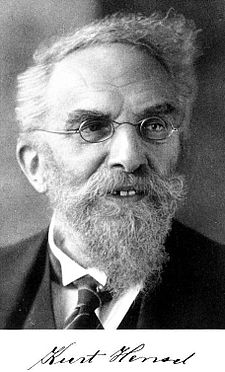
\includegraphics[height=4cm]{../../modules/history/pictures/hensel.jpg}
	
	\hfil\hfil Kurt Hensel (1861 - 1941)
	
	\hfil\hfil German mathematician
	

	\hfil\hfil Known for: 	invented the $p$-adic numbers
	
	
\end{frame}
\begin{frame}
	\hfil\hfil 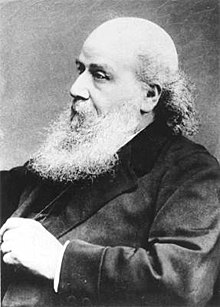
\includegraphics[height=4cm]{../../modules/history/pictures/sylvester.jpg}
	
	\hfil\hfil James Joseph Sylvester (1814 - 1897)
	
	\hfil\hfil English mathematician
	
	\hfil\hfil Invented the terms: 
	
	\hfil\hfil ``matrix'', ``graph'', ``discriminant'', ``totient''.

	\hfil\hfil Known also for: 	
	
	\hfil\hfil matrix theory, combinatorics, 
	
	\hfil\hfil invariant theory, number theory, 
	
	\hfil\hfil partition theory
	
	
\end{frame}
\begin{frame}[fragile]
\vskip -0.2cm
\tiny 
\begin{example}
\begin{itemize}
\item Factor $\alertNoH{12,29,31,44}{325x^{2}-38x-312}$ modulo  $3$.
\item \alertNoH{ 33}{Lift the modulo $3$ factorization to modulo $3^6=729$}. 
\item<handout:4|34->{ \alertNoH{34,44} {Why should we care?}}
\end{itemize}
\uncover<2->{
$
\begin{array}{rcll}
\alertNoH{2,3}{325x^{2}-38x-312} &\alertNoH{2}{\equiv}&\fcAnswer{3}{\alertNoH{4,5} { x^2+x}} &\mod 3 \\
\uncover<4->{&\equiv&  (\fcAnswer{5}{\alertNoH{11}{x+1}})(\fcAnswer{5}{\alertNoH{11}{x}}) &\mod 3} \\
\uncover<6->{&=& (\alertNoH{8}{1}\cdot x+\alertNoH{8}{1})(\alertNoH{9}{1}\cdot x+\alertNoH{9}{0}) &\mod 3}

\end{array}$
}

\uncover<7->{
\alertNoH{7}{Sylvester matrix:} $\uncover<7->{S=\begin{pmatrix}\alertNoH{8}{1}&\alertNoH{9}{1}\\\alertNoH{8}{1}&\alertNoH{9}{0}\end{pmatrix}}\uncover<10->{, \alertNoH{19}{S^{-1}}=\begin{pmatrix}0&1\\1&-1\end{pmatrix}= \alertNoH{19}{ \begin{pmatrix}0&1\\1&2\end{pmatrix}}} \mod 3$.
}
\begin{itemize}
\only<handout:1|-27>{ 
\item<11->[1] $
\begin{array}{rcll}\alertNoH{13,14}{f_1}&\equiv &\alertNoH{13,14}{(\alertNoH{11}{x})(\alertNoH{11}{x+1} )}&\mod3\\
\alertNoH{23}{a_{1}} &\alertNoH{23}{\equiv} & \alertNoH{11,23}{x} & \mod 3 \\
\alertNoH{23}{b_{1}} &\alertNoH{23}{\equiv} & \alertNoH{11,23}{x+1} & \mod 3 \end{array}$.


\item<12->[2] $
\begin{array}{rcllllll}\alertNoH{13,14}{f_2}&\equiv & \alertNoH{12,13,14}{x^{2}+7x+3} &&&&\alertNoH{12}{\mod 9} \\
\uncover<13->{\alertNoH{17,18} {g_2}&\equiv & \alertNoH{13}{f_2}-\alertNoH{13}{f_1}\uncover<14->{&=\alertNoH{15,16}{ \alertNoH{14}{x^{2}+7x+3}- \alertNoH{14}{(x)(x+1)}}} \uncover<15->{ &\alertNoH{15,16}{\equiv} &\fcAnswer{16}{\alertNoH{17,18}{ 6x+3}}}&\mod 9} \\
\uncover<17->{ \alertNoH{17,18}{ \frac{g_2}{3}}&\alertNoH{17,18}{ \equiv} & \fcAnswer{18}{\alertNoH{20}{ 2}x+\alertNoH{20}{1} } &&&&\alertNoH{17,18}{ \mod 3}} \\
\uncover<19->{\alertNoH{19}{ S^{-1}}\cdot \frac{g_2}{\alertNoH{25}{ 3} }&=& \alertNoH{21}{ \alertNoH{19}{\begin{pmatrix}0&1\\1&2\end{pmatrix}} \begin{pmatrix} \alertNoH{20}{ 2} \\\alertNoH{20}{1} \end{pmatrix}} \uncover<21->{ &&\equiv &\alertNoH{21}{ \begin{pmatrix}\alertNoH{24}{1}\\\alertNoH{24}{1} \end{pmatrix}}} &\mod3} \\ 
\uncover<22->{ 
\alertNoH{22,23,24,25,26}{a_{2}}&\equiv &\alertNoH{23}{x}  &+\alertNoH{25}{3} \cdot (\alertNoH{24}{1} ) \uncover<26->{&\equiv &\alertNoH{26}{x+3} &}\mod9 \\
\alertNoH{22,23,24,25,26}{b_{2}}&\equiv &\alertNoH{23}{x+1}&+\alertNoH{25}{3} \cdot (\alertNoH{24}{1}) \uncover<26->{&\equiv &\alertNoH{26}{x+4}&}\mod9
}
\end{array}
$	

\item<27>[3] $
\begin{array}{rclcllll}f_{3}&\equiv &x^{2}+16x+12&&&&\mod27\\g_{3}&\equiv &f_{3}-(x+3)(x+4)&&\equiv &9x&\mod27\\\frac{g_{3}}{9}&\equiv &x&&&&\mod3\\S^{-1}\cdot \frac{g_{3}}{9}&=&\begin{pmatrix}0&1\\1&2\end{pmatrix}\begin{pmatrix}1\\0\end{pmatrix}&&\equiv &\begin{pmatrix}0\\1\end{pmatrix}&\mod3\\
\alertNoH{27}{a_{3}} & \equiv &x+3&+9\cdot (0)&\alertNoH{27}{\equiv} & \alertNoH{27}{x+3} &\mod27\\
\alertNoH{27}{b_{3}} & \equiv &x+4&+9\cdot (1)&\alertNoH{27}{\equiv} & \alertNoH{27}{x+13} &\mod27\end{array}
$
}

\only<handout:2|28>{
\item[4]
$\begin{array}{rclcllll}f_{4}&\equiv &x^{2}+43x+12&&&&\mod81\\g_{4}&\equiv &f_{4}-(x+3)(x+13)&&\equiv &27x+54&\mod81\\\frac{g_{4}}{27}&\equiv &x+2&&&&\mod3\\S^{-1}\cdot \frac{g_{4}}{27}&=&\begin{pmatrix}0&1\\1&2\end{pmatrix}\begin{pmatrix}1\\2\end{pmatrix}&&\equiv &\begin{pmatrix}2\\2\end{pmatrix}&\mod 3\\
\alertNoH{28}{a_{4}} &\equiv &x+3&+27\cdot (2)&\equiv &\alertNoH{28}{x+57}&\mod 81\\
\alertNoH{28}{b_{4}} &\equiv &x+13&+27\cdot (2)&\equiv &\alertNoH{28}{x+67}&\mod 81\end{array}$
}

\only<handout:3|29-30>{ 
\item[5] ~
$\begin{array}{rcllllll}
\alertNoH{29}{h_{5}} & \equiv &\alertNoH{29}{ \alertNoH{30}{82}x^{2}+205x+174} 
&&&& \alertNoH{29}{\mod 243} \\
\alertNoH{30}{ f_{5}} =\frac{\alertNoH{30}{ h_{5}}}{
\alertNoH{30}{ 82}
}&\equiv &x^{2}+124x+174&&&&\mod 243\\
g_{5}&\equiv &f_{5}-f_{4}&=x^{2}+124x+174-(x+57)(x+67)&\equiv &0&\mod243\\
\frac{g_{5}}{81}&\equiv &0&&&&\mod3\\
S^{-1}\cdot \frac{g_{5}}{81}&=&\begin{pmatrix}0&1\\1&2\end{pmatrix}\begin{pmatrix}0\\0\end{pmatrix}&&\equiv &\begin{pmatrix}0\\0\end{pmatrix}&\mod3\\a_{5}&\equiv &x+57&+81\cdot (0)&\equiv &x+57&\mod243\\b_{5}&\equiv &x+67&+81\cdot (0)&\equiv &x+67&\mod243\end{array}
$
}

\only<handout:4|31->{ 
\item[6]
$\begin{array}{rcllllll}\alertNoH{31}{ h_{6}}&\equiv & \alertNoH{31}{ \alertNoH{32}{325} x^{2}+691x+417} &&&&\mod729\\
f_{6}=\frac{h_{6}}{\alertNoH{32}{325}}&\equiv &x^{2}+610x+174&&&&\mod729\\g_{6}&\equiv &f_{6}-f_{5}&=x^{2}+610x+174-(x+57)(x+67)&\equiv &486x&\mod729\\\frac{g_{6}}{243}&\equiv &2x&&&&\mod3\\S^{-1}\cdot \frac{g_{6}}{243}&=&\begin{pmatrix}0&1\\1&2\end{pmatrix}\begin{pmatrix}2\\0\end{pmatrix}&&\equiv &\begin{pmatrix}0\\2\end{pmatrix}&\mod3\\
a_{6}&\equiv &x+57&+243\cdot (0)&\equiv &\alertNoH{34}{x+57} & \mod 729\\
b_{6}&\equiv &x+67&+243\cdot (2)&\equiv &\alertNoH{34}{x+553}& \mod 729 \end{array}$
}
\end{itemize}

\only<handout:4|31->{ 
\uncover<33->{ Answer: $\alertNoH{33}{ \alertNoH{34}{h_6=325 \left( x+57 \right)\left(  x+553  \right)} \equiv 325x^{2}-38x-312 \mod 729} $.}

\uncover<34->{
\!\!$
\begin{array}{@{}rcll|l}
\alertNoH{34}{325 h_6} &=& \alertNoH{34,35}{325^2} \left(\alertNoH{34}{ x+57} \right)\left(\alertNoH{34}{ x+553} \right) \\
\uncover<35->{ &=& \left(\alertNoH{35}{325} x+ \alertNoH{36}{ \alertNoH{35}{325}\cdot 57} \right)\left(\alertNoH{35}{325} x+\alertNoH{36}{\alertNoH{35}{325}\cdot 553} \right)} \\
\uncover<36->{&\equiv& \left(325x+\alertNoH{36}{300}\right)\left(325 x+\alertNoH{36,37,38}{391}\right) & \alertNoH{36}{\mod 729} }  \uncover<37->{&  \alertNoH{37,38}{ 391>\frac{729}{2}} \uncover<38->{\text{\alertNoH{38}{ so convert it to negative}} }} \\
\uncover<38->{
&=& \left(\alertNoH{39}{325x+300} \right) \left( \alertNoH{40}{ 325 x \alertNoH{38}{-338}} \right)  &\mod 729 & \alertNoH{ 38}{391\equiv 391-729=-338 \mod 729} }\\
\uncover<39->{ 
&=&  \alertNoH{39,41}{25}\left(\alertNoH{39}{13x+12}\right)\alertNoH{40,41}{13}\left(\alertNoH{40}{25x-26} \right) &\mod 729} \\
\uncover<41->{&=&\alertNoH{41}{ 325}  \alertNoH{42}{ \left(13x+12\right)\left(25x-26\right)}&\mod 729}\\
\uncover<42->{
\alertNoH{42,43,44}{\left(13x+12\right)\left(25x-26\right)}&\alertNoH{43,44}{=} & \fcAnswer{44}{325x^{2}-38x-312}& \alertNoH{43,44}{\text{over }\mathbb Z }
}
\end{array}
$
}}



\end{example}
\vskip 10cm
\end{frame}
\begin{frame}
\tiny 
\begin{example}
\begin{itemize}
\item Factor
$\alertNoH{6}{ \alertNoH{4}{3213876088517982378070044454832611609600218716222701623311919} x^{2}+4017381846086652655535922512432598407525713541992513563440642 x +803499635068049951114704144708514061442615061308575325033080}$ modulo $5$.
\item Lift the factorization back mod $5^{88}$.
\item Factor the original polynomial over the integers.

\item<2->[1] $
\begin{array}{rcll}f_{1}&\equiv &(x)(x+3)&\mod5\\a_{1}&\equiv &x&\mod5\\b_{1}&\equiv &x+3&\mod5\end{array}
$

\uncover<3->{$\vdots$} 
\item<3->[88] 
$
\begin{array}{rcllllll}
a_{88}&\equiv  &x + 5018955281133163909890971477176569556248445440724618734961815 &\mod 5^{88}\\
b_{88}&\equiv &x + 27802729904771666433942097294515736463292086400511967042588228 & \mod 5^{88}
\end{array}$
\end{itemize}

\uncover<4->{
$
\begin{array}{r}
{\alertNoH{4}{3213876088517982378070044454832611609600218716222701623311919}}^2 a_{88}b_{88} =\\
\uncover<5->{
1267650600228230019170099489319\cdot \\
\left( 2535301200456459008884538505401x+633847839454405393006439465940 \right)\\ 2535301200456459008884538505401\cdot \\
\left( 1267650600228230019170099489319x+1267653820133985214676430042982\right) \\
\mod 5^{88}
}
\end{array}$

The procedure for choosing numbers $\mod 5^{88}$ was described earlier.
}

\uncover<6->{ The latter factorization is $\mod 5^{88}$, but it also works over $\mathbb Z$:
$\begin{array}{r}
\left( \alertNoH{6 }{ 2535301200456459008884538505401x+633847839454405393006439465940 }\right)\\
\left( \alertNoH{6 }{1267650600228230019170099489319x+1267653820133985214676430042982} \right)=\\ 
\alertNoH{6 }{3213876088517982378070044454832611609600218716222701623311919x^{2}+}\\
\alertNoH{6 }{4017381846086652655535922512432598407525713541992513563440642x+}\\
\alertNoH{6 }{803499635068049951114704144708514061442615061308575325033080}\\
\alertNoH{6 }{\text{over }\mathbb Z}
\end{array}$
}
\end{example}
\end{frame}
\begin{frame}
\frametitle{Is factorization over $\mathbb Z$ related to factorization $\mod p$?}
\begin{itemize}
\item<1-> Suppose we know a factorization of a polynomial over $\mathbb Z$:
\[
h=c_1c_2\cdots c_k
\]
\item<2-> Then $h$ can also be factored $\mod p$ (for any $p$): simply take:
\[
h\equiv c_1c_2\cdots c_k \mod p
\]
\item<3-> Here, factorization $\mod p$ carries good information for the factorization of the original $h$ assuming:
\begin{itemize}
\item<4-> $h$ does not reduce to zero $\mod p$.
\item<5-> Each factor $c_i$ does not reduce its degree $\mod p$.
\end{itemize}
\item<6-> Since there are infinitely many primes, we can always find a $p$ that satisfies these two.
\end{itemize}
\end{frame}

\begin{frame}
\frametitle{Factorization over $\mathbb Z$ using finite fields: the main idea}
\begin{itemize}
\item The Hensel lift lemma leads to a factorization idea for $h$.
\item<2-> Suppose $h$ has $k$ unknown factors. 
\item<3-> Let $C$ be the leading coefficient of $H$.
\item<4-> Pick a prime $p$.
\item<5-> Factor fully $h \equiv C\cdot c_1\cdots c_s \mod p$ - easier than factoring over $\mathbb Z$.
\item<6-> For simplicity, suppose $s=k$ ($h$ - no additional factors $\mod p$).
\item<7-> For simplicity, suppose $c_i$'s are distinct ($h$ - square-free $\mod p$).
\item<8-> Hensel-lift factorization to $h \equiv C d_1\cdots d_s \mod p^n$
\item<9-> Represent every negative number $z$ larger than $-\frac{p^n}{2}$ by itself $\mod p$.
\item<10-> Compute $C^{n-1}h= \left(Cd_1\right)\cdots\left(Cd_s\right) \mod p^n$.
\item<11-> Choose $n$ large enough so $\frac{p^n}{2}$ is larger than the absolute value of every coefficient of $C f_i$ for every unknown factor $f_i$ of $h$ over $\mathbb Z$.
\item<12-> Then the integer coefficients of $C f_i$ are the the integer coefficients of one of the $Cd_i$'s.
\end{itemize}
\end{frame}

\begin{frame}
\frametitle{Factorization over $\mathbb Z$ using finite fields: the problems}
\begin{itemize}
\item We just described a plan for extracting a factorization over $\mathbb Z$ from a factorization $\mod p$.
\item<2-> The plan had a few problems / open questions.
\begin{itemize}
\item<3-> How to choose the prime $p$?
\item<4-> How to efficiently factor $\mod p$? 
\item<5-> What happens when factoring $\mod p$ yields more factors than we have over $\mathbb Z$? Example:
\begin{itemize}
\item  $
\begin{array}{rcl}
x^3+\alertNoH{7}{2x}-3&=& \uncover<6->{\alertNoH{8}{  x^3}+\alertNoH{6}{ \alertNoH{8} {x^2} \alertNoH{9}{-x^2}} +\alertNoH{7}{\alertNoH{8}{3x} \alertNoH{9}{-x}}\alertNoH{9}{-3}}\\
\uncover<8->{&=& \left(\alertNoH{8,10}{x^3+x^2+3x}\right)\alertNoH{9}{\alertNoH{11}{-} x^2\alertNoH{11}{-}x\alertNoH{11}{-}3}}  \\
\uncover<10->{&=& \alertNoH{10}{\alertNoH{13}{x}\left(\alertNoH{12}{x^2+x+3} \right)} \alertNoH{11,13}{-}\left(\alertNoH{12}{x^2\alertNoH{11}{+}x\alertNoH{11}{+}3} \right)}\\
\uncover<12->{&=&(\alertNoH{13,15}{x-1})\left(\alertNoH{12,15}{x^2+x+3}\right)}
\end{array}$

\fcAnswerUncover{5}{14}{2} factors over $\mathbb Z$.
~\\
~\\
\item $
\begin{array}{rcll}
\alertNoH{15}{x^3+2x-3}&\alertNoH{15}{=}& \uncover<15->{ (\alertNoH{15}{x \alertNoH{16}{-1} })\left(\alertNoH{15}{x^2+x+\alertNoH{17}{3}}\right)} &\alertNoH{15,16,17}{\mod 3}\\
\uncover<16->{&\equiv& (x+\alertNoH{16}{2})\left(\alertNoH{18}{x^2+x}\right)& \alertNoH{16,17}{\mod 3}}\\
\uncover<18->{&=&(x+2) \alertNoH{18}{x(x+1)}&\mod 3}
\end{array}$

\fcAnswerUncover{5}{18}{3} factors over $\mathbb Z_3$
\end{itemize}
\item<19-> How to choose $n$ large enough so that factorization $\mod p^n$ helps us read off factorization over $\mathbb Z$?
\end{itemize}
\end{itemize}
\end{frame}

\begin{frame}
\begin{itemize}
\item When doing Hensel lifts of $h\in \mathbb Z[x]$ with more than 2 co-prime factors: $a_1\cdot a_2 \cdots a_k \mod p $
we could:
\begin{itemize}
\item<2-> Group into two factors: $a_1 \cdot \left(a_2\cdots a_k\right) $.
\item<3-> Lift $a_1$ to $d_1 \mod p^n$.
\item<4-> Compute $h_1 = \frac{h}{d_1 } \mod p^n$ - this is a polynomial as $h$ is divisible by $d_1$).
\item<5-> Apply the same procedure to lift $a_2$ relative to $h_1$, and so on by recursion.
\end{itemize}
\item<6-> This is uncomfortable to work with: let's do the lift with all $k$ factors simultaneously. 
\end{itemize}
\end{frame}
\begin{frame}
\tiny 

Let $h\in \mathbb Z$ and $h\equiv a_1\cdots a_k \mod p$. \uncover<2->{Suppose we want to \alertNoH{2}{Hensel-lift} a factorization $\alertNoH{2}{a_1\cdots a_k \mod p}$ to a factorization  $\alertNoH{2}{ \alertNoH{3}{\left(a_1+ pb_1\right) \cdots \left(a_k+pb_k\right)} \mod p^2}$.}


~\\

\uncover<3->{
$\begin{array}{rcll}
\alertNoH{3}{ \left( \alertNoH{4,6,7}{ a_1}+\alertNoH{5}{pb_1}\right)\left( \alertNoH{4,5,7}{a_2} +\alertNoH{6}{p b_2}\right)  \cdots \left(\alertNoH{4,5,6}{a_k} + \alertNoH{7}{ pb_k} \right)} &=&\alertNoH{4}{ a_1\cdot a_2\cdots a_k}+\\
&&\alertNoH{5,6,7}{  p}\left( \alertNoH{5}{\alertNoH{10,17}{b_1} \alertNoH{11,12}{ a_2 \cdots a_k} } + \alertNoH{6}{\alertNoH{11,12}{a_1} \alertNoH{10,17}{b_2} \alertNoH{11,12}{\cdots a_k}}+\dots + \alertNoH{7}{ \alertNoH{11,12}{a_1a_2\cdots}\alertNoH{10,17}{ b_k}} \right)+ \\
&&\alertNoH{8}{ \cancel{ p^2\left(\dots\right)}} &\alertNoH{8}{\mod p^2}\\
\uncover<9->{ &\equiv& h &\mod p^2}
\end{array}$
}

~\\
~\\

\uncover<10->{ To find the lift above, we need to \alertNoH{10}{solve for $b_1, \dots, b_k$}.} \uncover<11->{ Let 
\alertNoH{11,12}{$A_j$ be the product of the $a_i$'s with the $j^{th}$ factor omitted}, that is, }

\uncover<12->{
\hfil\hfil$
\alertNoH{12,14,22}{ A_j=\frac{a_1\cdots a_k}{a_j}}
$
}

\uncover<13->{\alertNoH{18}{Let $H=\deg h$.}} \uncover<14->{ Let the \alertNoH{15,17,20}{coefficients} of $\alertNoH{14,15}{A_j}$, $\alertNoH{16,17}{b_j}$, $\alertNoH{19,20}{h-a_1\cdots a_k}$ be as follows: } 

\[
\begin{array}{rcl}
\uncover<14->{\alertNoH{14,22}{A_j} &\alertNoH{14,22}{=}& \alertNoH{14,22}{ \alertNoH{15}{A_{j,0}} x^{\alertNoH{18}{s_j}}+ \alertNoH{15}{A_{j, 1}} x^{s_j-1}+\dots}} \\
\uncover<16->{ \alertNoH{16}{b_j} &\alertNoH{16}{=}& \alertNoH{16}{\alertNoH{17}{b_{j,0}} x^{\alertNoH{18}{t_j}}+\alertNoH{17}{b_{j,1}}x^{t_j-1}+\dots}} \\
\uncover<18->{ \alertNoH{18}{H} &\alertNoH{18}{=}& \alertNoH{18}{s_j+ t_j}} \\
\uncover<19->{ \alertNoH{19}{h-a_1\cdots a_k}   &\alertNoH{19}{=}& \alertNoH{19}{\alertNoH{20}{h_0} x^{H} + \alertNoH{20}{h_1} x^{H-1} +\dots}}
\end{array}
\]

\uncover<21->{
Then to solve for $b_1, \dots, b_k$, we need to solve the linear system:


$	
\alertNoH{22}{\left( \begin{array}{cccc|c|ccccc}
A_{1,0}   &0        &\dots &0        && A_{k,0}  & 0&\dots &0\\
A_{1,1}   &A_{1,0}  &\dots &0        && A_{k,1}  & A_{k,0} &\dots&0 \\
\vdots    &         &\ddots&         && \vdots&&\ddots \\
A_{1,s_1} &         &      &A_{1,0}  &\dots &\\
0         &A_{1,s_1}&      &         &&A_{k,s_k}&&&A_{k,0}\\
&         &         &      &         &0&A_{k,s_k}& \\
\vdots    &         &\ddots&\vdots   &&\vdots  & &\ddots &\vdots \\
0         &\dots    &      &A_{1,s_1}&&0&\dots &0&A_{k,s_k}
\end{array}
\right)} \left( 
\begin{array}{c}
b_{1,0} \\
b_{1,1}\\
\vdots\\ 
b_{1,s_1}\\\hline
\vdots \\\hline
b_{k,0} \\
b_{k,1}\\
\vdots\\
b_{k,s_k}
\end{array}\right) =  \left( 
\begin{array}{c}
h_0 \\
h_1\\
\vdots\\ 
h_{s_1}\\\hline
\vdots \\\hline
h_{H-s_k+1}\\
h_{H-s_k+2}\\
\vdots\\
h_{H}
\end{array}\right)
$
}

\end{frame}

\begin{frame}
\tiny
\begin{definition}[Sylvester multi-matrix]
We call
\[
\alertNoH{1}{\left( \begin{array}{cccc|c|ccccc}
A_{1,0}   &0        &\dots &0        && A_{k,0}  & 0&\dots &0\\
A_{1,1}   &A_{1,0}  &\dots &0        && A_{k,1}  & A_{k,0} &\dots&0 \\
\vdots    &         &\ddots&         && \vdots&&\ddots \\
A_{1,s_1} &         &      &A_{1,0}  &\dots &\\
0         &A_{1,s_1}&      &         &&A_{k,s_k}&&&A_{k,0}\\
&         &         &      &         &0&A_{k,s_k}& \\
\vdots    &         &\ddots&\vdots   &&\vdots  & &\ddots &\vdots \\
0         &\dots    &      &A_{1,s_1}&&0&\dots &0&A_{k,s_k}
\end{array}
\right)} 
\]
the Sylvester multi-matrix of the polynomials $a_1, \dots a_k$ where each  $A_j$ is given by:


\[
\alertNoH{1}{
A_j=\frac{a_1\cdots a_k}{a_j}
}
\]

and $A_{j,k}$ are the coefficients of the polynomial $A_j$:

\[
\alertNoH{1}{
A_j =A_{j,0} x^{s_j}+A_{j, 1} x^{s_j-1}+\dots 
}
\]
\end{definition}
\end{frame}

\begin{frame}
\tiny 
\begin{example}
\begin{itemize}
\item \alertNoH{12}{ Factor }
$\begin{array}{rclclcl}
\alertNoH{12, 39, 61}{x^3+\alertNoH{4}{2x} \alertNoH{40}{-3}}&\uncover<2->{=}& \uncover<3->{ \alertNoH{5}{  x^3}+\alertNoH{3}{ \alertNoH{5} {x^2} \alertNoH{6}{- x^2}} +\alertNoH{4}{\alertNoH{5}{3x} \alertNoH{6}{- x}}\alertNoH{6}{-3}}
\uncover<5->{&=& \left(\alertNoH{5,7}{x^3+ x^2+3x}\right)\alertNoH{6}{ \alertNoH{8}{-} x^2 \alertNoH{8}{-} x\alertNoH{8}{-}3}}  \\
\uncover<7->{&=& \alertNoH{7}{\alertNoH{10}{x}\left(\alertNoH{9}{x^2+x+3} \right)} \alertNoH{8,10}{-}\left(\alertNoH{9}{x^2\alertNoH{8}{+}x\alertNoH{8}{+}3} \right)}
\uncover<9->{&=&\alertNoH{61}{ (\alertNoH{10,12}{x-1} )\left( \alertNoH{9, 12}{x^2 + x+3}\right)}}
\end{array} $

\item \alertNoH{13}{ Factor $x^3+2x-3$ over $\mod 3$}.
\item Lift the factorization $\mod 9$. 
\item \alertNoH{61}{ Explain the connection between the $\mod 9$ and regular factorization.}
\end{itemize}

\uncover<13->{
$\begin{array}{rclclcll}
\alertNoH{13,37,38,42}{f_{1}} \only<-37|handout:1>{ &\alertNoH{13}{= }&\alertNoH{13}{x^3+2x\alertNoH{14}{-3}} \uncover<14->{& \equiv& \alertNoH{15}{ x^3 + 2x}} \uncover<15->{& \equiv& \alertNoH{15}{x(x^2+2)}}& \alertNoH{13,14}{\mod 3} \\
\uncover<16->{&\equiv& x(x^2+\alertNoH{16,17}{ 3x} +2)\uncover<17->{&\equiv& x( \alertNoH{18}{x^2+}\alertNoH{17}{\alertNoH{18}{x}+\alertNoH{19}{2x}}\alertNoH{19}{+2})}}
\uncover<18->{&\equiv&x(\alertNoH{18}{\alertNoH{21}{x}(\alertNoH{20}{x+1})}\alertNoH{21}{+}\alertNoH{19}{\alertNoH{21}{2}(\alertNoH{20}{x+1})})}&\mod 3\\}
\uncover<20->{&\alertNoH{37,38}{ \equiv} &\alertNoH{37,38,42}{ \alertNoH{22}{ x}( \alertNoH{20,22}{x + 1})(\alertNoH{21,22}{x+2})} &&&&&\mod 3}\\
\uncover<22->{
\alertNoH{26,27,28,29,37,38,49}{a_{1}} &\alertNoH{26, 27, 28, 29, 37, 38, 49}{ \equiv} &\alertNoH{22,26,27,28,29,37,38, 49}{x}&&&&&\mod 3\\
\alertNoH{23,24,28,29,37,38,49}{b_{1}}&\alertNoH{23,24,28,29,37, 38, 49}{\equiv} &\alertNoH{22,23,24,28,29,37,38, 49}{x +1}&&&&&\mod 3\\
\phantom{a_1\cdot } \alertNoH{23,24,26, 27,37,38, 49}{c_{1}}& \alertNoH{23, 24, 26, 27, 37, 38, 49}{\equiv} &\alertNoH{22,23,24,26,27,37,38, 49}{ x+2}&&&&&\mod 3\\
}
\only<-37|handout:1>{
\uncover<23->{ \alertNoH{23,24}{b_1\cdot c_1} &\alertNoH{23,24}{=}& \fcAnswer{24}{ x^2 + \alertNoH{25}{3x}+2} \uncover<25->{&\equiv& x^2+2 }\uncover<32->{&=&\alertNoH{32}{1}\cdot x^2+\alertNoH{32}{0}\cdot x +\alertNoH{32}{2}} &\alertNoH{25}{\mod 3}\\
\alertNoH{26,27}{ a_1\cdot c_1} &\alertNoH{26,27}{=}& \fcAnswerUncover{23}{27}{x^2 + 2x}&&\uncover<33->{&=&\alertNoH{33}{1}\cdot x^2+\alertNoH{33}{2}\cdot x+\alertNoH{33}{0}} &\mod 3\\
\alertNoH{28,29}{a_1\cdot b_1} &\alertNoH{28,29}{=}& \fcAnswerUncover{23}{29}{x^2 + x}&&\uncover<34->{&=&\alertNoH{34}{1}\cdot x^2+\alertNoH{34}{1}\cdot x+\alertNoH{34}{0}} &\mod 3}
}
\end{array}
$

\uncover<23->{ Sylvester multi-matrix: $S= \fcAnswerUncover{23}{31}{
\begin{pmatrix}
\alertNoH{32}{1} &\alertNoH{33}{1}&\alertNoH{34}{1}\\
\alertNoH{32}{0} &\alertNoH{33}{2}&\alertNoH{34}{1}\\
\alertNoH{32}{2} &\alertNoH{33}{0}&\alertNoH{34}{0}\end{pmatrix}
}$.} \uncover<35->{
$\alertNoH{35}{S^{-1}=} \alertNoH{35,36}{ \begin{pmatrix}0&0&\frac{1}{2} \\ -1&1&\frac{1}{2} \\ 2&-1&-1\end{pmatrix}} \uncover<36->{\equiv  \alertNoH{36}{ \begin{pmatrix}0 &0&2\\ 2&1&2\\2&2&2\end{pmatrix}} \alertNoH{36}{ \mod 3}} $
}
}

\only<handout:2|39->{
$
\begin{array}{rcllllll}
\alertNoH{41}{f_{2}} &\equiv &\alertNoH{39,41}{ x^{3}+2x+\alertNoH{40}{6}} &&&&\alertNoH{39,40}{ \mod 9} \\
\uncover<41->{ \alertNoH{44}{ g_{2}} &\equiv &\alertNoH{41}{ f_{2}} - \alertNoH{42}{f_{1}}& = \alertNoH{43}{\alertNoH{41}{ x^{3}+2x+6} - \alertNoH{42}{ (x)(x+1)(x+2)}} \uncover<43->{ &\equiv & \alertNoH{43, 44}{ 6x^{2}+ 6}}&\alertNoH{44}{ \mod 9}} \\
\uncover<44->{ \alertNoH{44,46}{ \frac{g_{2}}{ \alertNoH{50}{3}}} &\alertNoH{44}{ \equiv} & \alertNoH{44}{ 2x^{2}+2} \uncover<46->{ &= \alertNoH{46}{2} \cdot x^2 + \alertNoH{46}{0} \cdot x + \alertNoH{46}{2}  }&&&\alertNoH{44}{ \mod 3}} \\
\uncover<45->{ \alertNoH{45}{ S^{-1}\cdot \alertNoH{46}{ \frac{g_{2}}{3}}} &\alertNoH{45}{=}& 
\alertNoH{45,47}{ 
\begin{pmatrix} 0&0&2\\2&1&2\\2&2&2 \end{pmatrix} 
\begin{pmatrix} \alertNoH{46}{ 2} \\ \alertNoH{46}{0}\\ \alertNoH{46}{2} \end{pmatrix} 
} \uncover<47->{ 
&& \alertNoH{47}{\equiv} & 
\alertNoH{47}{ \begin{pmatrix} \alertNoH{51}{1} \\ \alertNoH{51}{2} \\ \alertNoH{51}{2} \end{pmatrix} }
} 
&\mod 3} \\
\uncover<48->{
\alertNoH{48}{a_{2}} & \alertNoH{48}{\equiv} &\alertNoH{48,49, 52}{ x} &\alertNoH{48, 52}{ + \alertNoH{50}{3}\cdot (\alertNoH{51}{1})} &\uncover<52->{ \alertNoH{52}{\equiv} &\alertNoH{52, 53}{x+3}} &\mod 9\\
\alertNoH{48}{b_{2}} & \alertNoH{48}{\equiv} &\alertNoH{48,49, 52}{ x+1} &\alertNoH{48, 52}{+ \alertNoH{50}{3} \cdot (\alertNoH{51}{2})} &\uncover<52->{ \alertNoH{52}{\equiv} &\alertNoH{52, 53}{x+7}} &\mod 9\\
\alertNoH{48}{c_{2}} & \alertNoH{48}{\equiv} &\alertNoH{48,49, 52}{ x+2} &\alertNoH{48, 52}{ + \alertNoH{50}{3} \cdot (\alertNoH{51}{2})} & \uncover<52->{ \alertNoH{52}{\equiv} &\alertNoH{52, 53}{ x +8} } &\mod 9\\
\uncover<53->{ f_2&\equiv & (\alertNoH{53}{\alertNoH{54,55}{x} + \alertNoH{56, 57}{3} } )(\alertNoH{53}{\alertNoH{54,56}{x}+\alertNoH{55, 57}{7}})( \alertNoH{53}{x +8})&\uncover<54->{ =  \left( x +\alertNoH{58}{ 8} \right) \left( \alertNoH{54}{ x^2} + \alertNoH{55,56,59}{10x} + \alertNoH{57,60}{21} \right)} &&& \mod 9 }\\
\uncover<58->{
&\equiv& \alertNoH{61}{ \left(x\alertNoH{58}{-1}\right) \left(x^2+\alertNoH{59}{x} +\alertNoH{60}{3}\right) } &&&&\alertNoH{58,59,60,61}{\mod 9}
}
\end{array}
}
$
}
\end{example}

\vskip 10cm
\end{frame}
\begin{frame}
\frametitle{Factorization over $\mathbb Z$ using finite fields: the problems}
\begin{itemize}
\item We just described a plan for extracting a factorization over $\mathbb Z$ from a factorization $\mod p$.
\item The plan had a few problems / open questions.
\begin{itemize}
\item How to choose the prime $p$?
\item How to efficiently factor $\mod p$? 
\item \alert<1->{What happens when factoring $\mod p$ yields more factors than we have over $\mathbb Z$?}
\item How to choose $n$ large enough so that factorization $\mod p^n$ helps us read off factorization over $\mathbb Z$?
\end{itemize}
\end{itemize}
\end{frame}

\begin{frame}
\begin{itemize}
\item Suppose $g$ is an irreducible factor of $f$ over $\mathbb Z$.
\item<2-> Suppose $g$ factors $\mod p$ into irreducibles: 
	
\[
\begin{array}{rcll|l}
g&\equiv& a_1\cdots a_s & \mod p  \\
g&\equiv& d_1\cdots d_s & \mod p^n &d_i \text{ is Hensel-lifted from } a_i
\end{array}
\]
\item<3-> Then the coefficients of $g$ can be read off the coefficients of the expanded product $d_1\cdots d_s$.
\end{itemize}
\end{frame}

\begin{frame}
\begin{question}
What happens when factoring $\mod p$ yields more factors than we have over $\mathbb Z$?
\end{question}
\begin{itemize}
\item<2-> Suppose $f\equiv d_1\cdots d_k \mod p^n$.
\item<3-> Suppose $C$ is the leading coefficient of $f$.
\item<4-> For every subset $\{i_1, \dots, i_s\}\subset \{1,\dots, k\}$:
\begin{itemize}
\item<5-> Expand $g=C\cdot d_{i_1}\cdots d_{i_s} \mod p^n$ fully.
\item<6-> Convert $g \in \mathbb Z_{p}^n[x]$ to integer-valued $\bar g \in \mathbb Z[x]$: \uncover<7->{replace every positive (representative) coefficient $z$ larger than $\frac{p^n}{2}$ to $z-p$.}
\item<8-> Divide $f$ by $\bar g$ over $\mathbb Q$; if remainder is zero, we've found a factor of $f$.
\end{itemize}  
\item<9-> We could try all subsets of $\{1,\dots, k\}$ (total $2^k$ possibilities).
\item<10-> However, if a factor involves more than half of the indices, its complement factor has fewer than half of the indices. 
\item<11-> $\Rightarrow$ we need to go \alertNoH{12}{up to subsets of size $\lfloor \frac{k}{2}\rfloor$}.  
\item<12-> $ \alertNoH{12}{\text{total subsets to try}=\begin{cases}
2^{k-1}& \text{ if } k-\text{odd}\\
2^{k-1} + \frac{1}{2}\binom{k}{\frac{k}{2}}& \text{ if } k-\text{odd}\\
\end{cases}}$ .
\item<13-> Try smaller subsets first $\Rightarrow$ discover irreducible factors first.
\end{itemize}
\end{frame}
\begin{frame}
\frametitle{Factorization over $\mathbb Z$ using finite fields: the problems}
\begin{itemize}
\item We just described a plan for extracting a factorization over $\mathbb Z$ from a factorization $\mod p$.
\item The plan had a few problems / open questions.
\begin{itemize}
\item How to choose the prime $p$?
\item How to efficiently factor $\mod p$? 
\item What happens when factoring $\mod p$ yields more factors than we have over $\mathbb Z$?
\item \alert<1->{How does one choose $n$ large enough so that factorization $\mod p^n$ helps us read off factorization over $\mathbb Z$?}
\end{itemize}
\end{itemize}
\end{frame}


\begin{frame}
\begin{question}
How does one choose $n$ large enough so that factorization $\mod p^n$ helps us read off factorization over $\mathbb Z$?
\end{question}

\begin{itemize}
\item<2-> Let $g$ be a factor of $f$. 
\item<3-> To convert coefficients of a factor over $\mathbb Z_{p^n}[x]$ to coefficients over $\mathbb Z$:
\item<4-> $\Rightarrow$ we need that $\frac{p^n}{2}$ be larger than the absolute value of each coefficient of $g $.
\item<5-> Let $G$ be the largest absolute value of a coefficient of $g$. Let $F$ be the largest absolute value of a coefficient of $f$.
\uncover<6->{
\begin{lemma}[Mahler: Gelfond's inequality]
$G \leq 2^{\deg f-1} \sqrt{\deg f+1} F$
\end{lemma}
}
\item<7-> The proof is not very easy. See inequality (II), K. Mahler, On some inequalities for polynomials in several variables, Journal London Mathematical Society 37, 1962, pages 341-344.
\end{itemize}

\end{frame}

\section{Factoring over finite fields: Cantor-Zassenhaus algorithm}
\begin{frame}
\frametitle{Factorization over $\mathbb Z$ using finite fields: the problems}
\begin{itemize}
\item We just described a plan for extracting a factorization over $\mathbb Z$ from a factorization $\mod p$.
\item The plan had a few problems / open questions.
\begin{itemize}
\item How to choose the prime $p$?
\item \alert<1->{How to efficiently factor $\mod p$?}
\item What happens when factoring $\mod p$ yields more factors than we have over $\mathbb Z$?
\item How does one choose $n$ large enough so that factorization $\mod p^n$ helps us read off factorization over $\mathbb Z$?
\end{itemize}
\end{itemize}
\end{frame}
\begin{frame}
\frametitle{Cantor-Zassenhaus factorization in $\mathbb Z_p[x]$}
\begin{itemize}
\item The \alertNoH{1}{Cantor-Zassenhaus algorithm} is an algorithm for efficient \alertNoH{1,3}{factorization} of a polynomial $f$ as a product of \alertNoH{2}{irreducibles} in \alertNoH{1}{$\mathbb Z[x]$}.
\item<2-> \alertNoH{2}{Irreducible polynomial = polynomial that can't be factored in an essential fashion}.
\item<3-> To \alertNoH{3}{factor a polynomial $f$} = write it as \alertNoH{3}{product of irreducibles}.
\item<4-> Irreducible factors of $g$ \alertNoH{4}{different degree} can be found quickly+efficiently.
\item<5-> The C-Z algorithm deals with factors of same degree.
\item<6-> The C-Z algorithm is a probabilistic, every run gives $\frac{1}{2}$ chance of (partial) factorization.
\end{itemize}
\end{frame}

\begin{frame}

\hfil\hfil David Geoffrey Cantor (1935 - 2012)

\hfil\hfil American mathematician

\hfil\hfil Known for: The Cantor-Zassenhaus algorithm


\end{frame}
\begin{frame}
\hfil\hfil 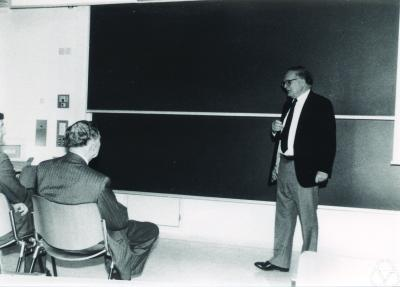
\includegraphics[height=4cm]{../../modules/history/pictures/zassenhaus.jpg}

\hfil\hfil Hans Julius Zassenhaus (1912 - 1991)

\hfil\hfil German mathematician

\hfil\hfil Known for: The Cantor-Zassenhaus algorithm


\end{frame}
\begin{frame}
\begin{itemize}
\item How do we factor in $\mathbb Z_p[x]$?
\item<2-> Suppose $a$ - irreducible polynomial $\mathbb Z_p[x]$, $\deg a=n$. \uncover<3-> Then:
\[
x^{p^n}-x \equiv 0 \mod a
\]
and $n$ is the smallest number for which the above holds. 

\item<4-> Above follows from theory of finite fields; google Galois Fields.
\item<5-> Suppose $a,b$-irreducible with $n=\deg a<\deg b$. \uncover<6->{ Then $a$ divides $x^{p^n}-x$ and $b$ doesn't divide it, so $gcd\left(a\cdot b, x^{p^n}-x\right)=a$.}
\item<7-> To separate all factors of different degrees of $f$, compute 
\[
\begin{array}{c}
\gcd(f, x^{p^{1}}-x)\\
\gcd(f, x^{p^{2}}-x)\\
\vdots\\
\gcd(f, x^{p^{\deg g}}- x)
\end{array}
\]
\item<8-> If any of these comes out different from $1$, then we've found a factor of $f$. 
\item<9-> Divide $f$ by that factor to simplify the problem.
\end{itemize}

\end{frame}
\begin{frame}
\hfil\hfil 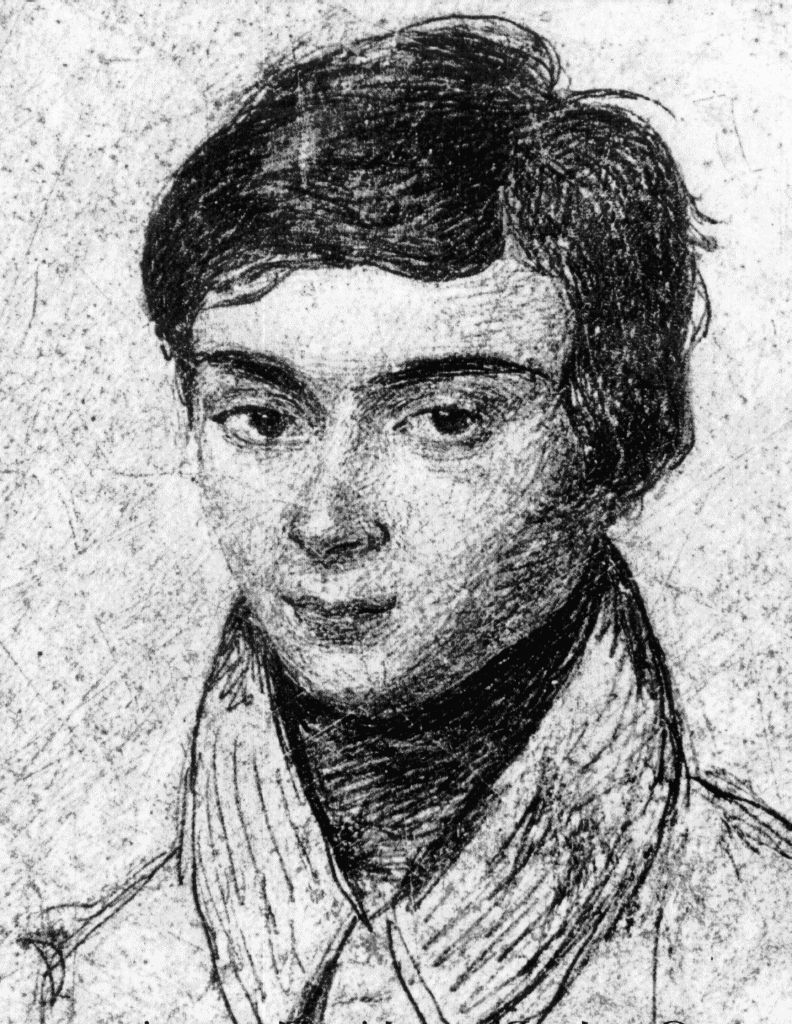
\includegraphics[height=4cm]{../../modules/history/pictures/galois.jpg}

\hfil\hfil \'Evariste Galois (1811-1832) [aged 20]

\hfil\hfil French mathematician

\hfil\hfil Known for: Galois Theory


\end{frame}
\begin{frame}
\begin{example}
\begin{itemize}
\item Factor $x^{5}+x^{3}+2x^{2}+2$ $\mod 7$.

\item<2-> Compute 
\[
\begin{array} {rcll}
\gcd(x^{7^1}-x, x^{5}+x^{3}+2x^{2}+2)&\equiv& 1&\mod 7\\
\uncover<3->{\gcd(x^{7^2}-x, x^{5}+x^{3}+2x^{2}+2)&\equiv&x^2+ 1&\mod 7\\
\vdots}
\end{array}
\]
\item<4-> Found non-unit gcd $x^2+1$ $\Rightarrow$ don't compute $x^{7^3}-x, x^{7^4}-x, \dots$. 

\item<5-> Divide $x^{5}+x^{3}+2x^{2}+2$ by $x^2+1$: remainder $=0$, quotient $=x^3+2$. 
\item<6-> $\gcd(x^{7^1}-x, x^{5}+x^{3}+2x^{2}+2)=1$ $\Rightarrow$ polynomial has no linear factors $\Rightarrow$ $\left(x^2+1\right),\left( x^3+2\right)$ are irreducible $\mod 7$.
\item<7-> Answer:
\[
x^{5}+x^{3}+2x^{2}+2=\left(x^2+1\right)\left( x^3+2\right) \mod 7
\]
\end{itemize}
\end{example}
\end{frame}
\begin{frame}
\footnotesize
\vskip -0.22cm
\begin{example}\vskip -0.1cm
Compute the remainder of  $x^{3^{6}}-x \mod 3$ divided by $x^2+x+1\mod 3$. Use the fact that $\alertNoH{26}{3^{6}=729=1+2^3+2^4+2^6+2^7+2^9}$.
\uncover<2->{\alertNoH{17,35,36}{All computations are $\mod 3$.}}

\begin{itemize}
\item<2-> \only<-8|handout:1>{ Regular polynomial division would yield $3^{6}=729$ rows. 
\item<3-> Instead, we will compute in the ring $\mathbb Z_3[x]/\langle x^2+x+1\mod 3 \rangle$.
\item<4->In other words, we will compute $\left( x^{3^{6}}-x\right) \mod \left(x^2+x+1 \right)$.

\uncover<5->{
Computing $\mod \left(x^2+x+1 \right)$ amounts to declaring 
}
}

\uncover<5->{
\hfil\hfil$
\alertNoH{8,9} {
\begin{array}{rcll}
\alertNoH{20}{ x^2+\alertNoH{6}{x+1}}&\alertNoH{20}{ \equiv}&\alertNoH{20}{  0} &\mod 3\\
\uncover<6->{ \alertNoH{12,22,29,31,33}{ x^2} &\alertNoH{12,22,29}{\equiv} & \alertNoH{7}{-}(\alertNoH{6}{x+1})\uncover<6->{\equiv\alertNoH{12,22,29,31,33}{ \alertNoH{7}{2}x+\alertNoH{7}{2}} } &\mod 3}
\end{array}
}
$
}


\only<handout:2|9->{
$
\begin{array}{rcrclcl}
\uncover<10->{ \alertNoH{27}{ x^{2^0}} &=& x^1&&& \equiv&\alertNoH{23,27}{ x}}\\
\uncover<11->{ x^{2^1} &=& \alertNoH{12,15,22}{x^2} &&& \alertNoH{12,15,22}{ \equiv}& \alertNoH{12,15,22,23}{ 2x+2}}\\
\uncover<13->{x^{2^2} &=& \alertNoH{13,14,21}{x^4}& \alertNoH{13,14}{\equiv}& \fcAnswer{14}{ \alertNoH{ 30}{ (\alertNoH{15}{ \alertNoH{16}{2}x+ \alertNoH{16}{2}} )^{ \alertNoH{16}{2}}}} \uncover<16->{ =\alertNoH{16,17}{4}(x+1)^2 \uncover<17->{=\alertNoH{18}{ ( x + 1)^2}}} }\\
\uncover<18->{ &&&\equiv&\alertNoH{18}{ x^2+ \alertNoH{19}{ 2x} +1}\uncover<19->{=\alertNoH{20}{x^2+\alertNoH{19}{x}}+\alertNoH{19}{x}\alertNoH{20}{+1}} } \uncover<20->{&\equiv& \alertNoH{21,23,30}{x} } \\
\uncover<21->{ \alertNoH{28}{ x^{2^3}} &=&\alertNoH{21}{ x^8} & \equiv& \alertNoH{21,22}{x^2} \uncover<22->{ &\alertNoH{22}{=} &\alertNoH{22,23,28}{2x+2}} }\\
\uncover<23->{
\alertNoH{27}{x^{2^4}}&=&x^{16}&&&\equiv&\alertNoH{23,27}{ x}\\
x^{2^5}&=&x^{32}&&&\equiv&\alertNoH{23}{ 2x+2}\\
} 
\uncover<24->{
\alertNoH{27}{x^{2^6}}&&&&&\equiv&\alertNoH{27}{x}\\
\alertNoH{28}{x^{2^7}}&&&&&\equiv&\alertNoH{28}{2x+2}\\
} 
\uncover<25->{
x^{2^8}&&&&&\equiv&x\\
\alertNoH{28}{x^{2^9}}&&&&&\equiv&\alertNoH{28}{2x+2}\\
}
\uncover<26->{x^{\alertNoH{26}{729} }&&&=& {\alertNoH{27,28}{ x}}^{ \alertNoH{26}{ \alertNoH{27}{1}+\alertNoH{28}{2^3}+ \alertNoH{27}{ 2^4}+ \alertNoH{27}{ 2^6 }+\alertNoH{28}{2^7}+\alertNoH{28}{2^9}}} \uncover<27->{ \equiv \alertNoH{27,29}{x^3} (\alertNoH{28}{2x +2})^{ \alertNoH{28}{3}}}}\\
\uncover<29->{
&&&=&\alertNoH{29}{x} \alertNoH{30}{(\alertNoH{29}{2x+ 2})^4}\uncover<30->{= x\cdot \alertNoH{30,31}{ x^2}}\uncover<31->{= \alertNoH{32}{x(\alertNoH{31}{2x+2})}}\\
\uncover<32->{&&&=& \alertNoH{32}{2 \alertNoH{33}{x^2}+2x} \uncover<33->{ =2(\alertNoH{33}{2x+2})+2x}\uncover<34->{ =\alertNoH{35}{6x}+\alertNoH{36}{4}} \uncover<35->{&\equiv&\alertNoH{36}{1}}}
}
\end{array}
$
}
\end{itemize}
\end{example}
\vskip 10cm
\end{frame}

\begin{frame}
\footnotesize
\vskip -0.22cm
\begin{example}\vskip -0.1cm
Compute the remainder of  $x^{3^{6}}-x \mod 3$ divided by $x^2+x+1\mod 3$.
\end{example}
\begin{itemize}
\item<2-> As we saw on the preceding slide, the answer is $1$.
\item<3-> We could have computed faster: 
\begin{itemize}
\footnotesize
\item<3-> $ x^{3}\equiv x\left(2x+2\right)\equiv 2x^2+2\equiv 6x+4\equiv 1 \mod \left(x^2+x+1\mod 3\right) $.
\item<4-> $x^{3^6}= \left( x^3\right)^{3^5}\equiv 1^{3^5}=1\mod \left(x^2+x+1\mod 3\right)$.
\end{itemize}
\item<5-> However, the previous method works for all examples.
\begin{itemize}
\footnotesize
\item<6-> We used consecutive squares to raise $x$ to a huge exponent.
\item<7-> We reduced all intermediates $\mod$ the polynomial before squaring again.
\item<8-> $\Rightarrow$ computations were small = good news when coding on a computer!
\end{itemize}
\item<9-> To find the gcd of a polynomial $g$ and $x^{p^n}-x$, we use the Euclidean algorithm.
\item<10-> The Euclidean algorithm only uses the remainder of $x^{p^n}-x$ divided by $g$.
\item<11-> $\Rightarrow$ finding $\gcd\left( x^{p^n}-x,g\right)$ is efficient computationally.
\item<12-> This is so efficient it's doable by hand on not-so-small-examples.
\end{itemize}


\vskip 10cm
\end{frame}

\begin{frame}
\frametitle{Factor polynomials of the same degree over $\mathbb Z_p$, $p>2$}
\begin{itemize}
\item Suppose $ g=a_1\cdot a_2\cdot \dots \cdot a_k$ with $a_i$-irreducible and $\deg a_i=\deg a_j$ for all $i,j$.
\item How do we factor $g$?
\item Suppose $g$ is not square-free, say $a_1=a_2$
\begin{itemize}
\item $g= a_1a_2 a_3\cdots= a_1^2  h$.
\item $g'= 2a_1 a_1' h+ a_1^2 h'=a_1(2a_1'h+a_1h')$ 
\item $\Rightarrow$ $a_1$ divides $g, g' $ $\Rightarrow$ $\gcd(g,g')$ is a factor of $g$.
\end{itemize} 
\end{itemize}
\end{frame}

\begin{frame}
\frametitle{Factor polynomials of the same degree over $\mathbb Z_p$, $p>2$}
\begin{itemize}
\item For simplicity, assume: $g=a_1\cdot a_2$, $a_1\neq a_2$, $\deg a_1=\deg a_2=d$, $\deg g=n=2d$. 
\item  Take random $h\in \mathbb Z_p$ with $\gcd(h,g)=1$. We have:

\hfil \hfil $
\begin{array}{rcll}
h^{p^d}-h &\equiv &0&\mod g\\
h\left(h^{p^d-1}-1 \right)& \equiv &0&\mod g \\
h^{p^d-1}-1&\equiv&0&\mod g\\
\left( h^{\frac{p^d-1}{2}}\right)^2 - 1&\equiv&0& \mod g\\
\left( h^{\frac{p^d-1}{2}} - 1\right)\left( h^{\frac{p^d-1}{2}}+ 1\right) &\equiv&0& \mod g\\
\end{array}
$

So $g$ divides this product: if lucky, $\gcd\left(h^{\frac{p^d-1}{2}} - 1,g\right)=a_1$ or $a_2$.

\item Chance for this to happen = $\frac{1}{2}$, so doing the above $s$ times factors $g$ with probability $1-\left(\frac{1}{2} \right)^s$. 
\item Take $s=10$: chance to factor = $1023$ in $1024$.
\end{itemize}
\end{frame}
\begin{frame}
\footnotesize
\begin{example}
Find two irreducible factors of $\alertNoH{2,3,4,73}{f=} \alertNoH{2,3,4,73}{x^{4}+x^{3}+x+2 \alertNoH{6}{\mod 3}}$ of degree $\alertNoH{9,73}{2}$.

\begin{itemize}
\item<2-> Compute in $\mathbb Z_3[x]/\langle \alertNoH{2}{x^{4}+x^{3}+x+2\mod 3} \rangle $.
\item<3-> $\Rightarrow$ compute $ \mod \alertNoH{3}{f}$, that is, $\mod  (\alertNoH{3}{x^{4}+x^{3}+x+2 \mod 3})$.

\uncover<4->{
$\begin{array}{rcll}
\alertNoH{4}{x^{4}\alertNoH{5}{ +x^{3}+x+2}} &\equiv&\alertNoH{4}{ 0}&\alertNoH{4}{ \mod f} \\
\uncover<5->{x^4&\equiv& \alertNoH{5}{\alertNoH{6}{-}x^3 \alertNoH{6}{-} x\alertNoH{6}{-2}} \uncover<6->{ \equiv \alertNoH{11}{\alertNoH{6}{ 2}x^3+\alertNoH{6}{2}x+\alertNoH{6}{1}}& \alertNoH{11}{\mod f}}}\\

\end{array}
$
}

\item<7-> Choose the \alertNoH{8}{``random polynomial'' $x$}. \uncover<8->{ Compute $\alertNoH{9}{ {\alertNoH{8}{x}}^{\frac{3^{\alertNoH{9}{2} }-1}{2}} +1}$:}

$ 
\uncover<9->{\alertNoH{9}{ x^{\alertNoH{10}{\frac{3^{2}-1}{2}}}+ 1} =\uncover<10->{\alertNoH{11}{x^{\alertNoH{10}{4}} } +1} \uncover<11->{ \equiv \alertNoH{11}{2x^3+2x+\alertNoH{12}{1}} \alertNoH{12}{+1}} \uncover<12->{
= 2x^3+2x+\alertNoH{12}{2}} \alertNoH{11}{\mod f}}
$

\item<12-> Compute $\gcd (f, 2x^3+2x+2)$. Use Euclidean algorithm $\mod 3$:

\tiny
\begin{columns}
\column[t]{0.4\textwidth}

$
\begin{array}{rcl}
\alertNoH{13,49}{x^4+x^3+x+2} &=& (\fcAnswerUncover{13}{30}{ 2x+2} ) \left( \alertNoH{32,50}{2x^3 +2x+2} \right)+\fcAnswerUncover{13}{31}{ \alertNoH{33,51}{ 2x^2 +2x+1}}\\
\uncover<32->{\alertNoH{32}{2x^3+2x+2}&=&(\fcAnswerUncover{32}{47}{x+2 }) \left(\alertNoH{33,51}{ 2x^2+2x+1} \right)+\fcAnswerUncover{32}{48}{0} }\\
\uncover<49->{\Rightarrow \gcd\left( \alertNoH{49}{ f}, \alertNoH{50}{2x^3+2x+2} \right) &=&\alertNoH{51}{2x^2 +2x+1}}\\
\uncover<52->{ \alertNoH{53}{ x^4+x^3+x+2}&=&\left( \fcAnswerUncover{52}{68}{ \alertNoH{70}{2} x^2+\alertNoH{70}{2}} \right)\left( \alertNoH{54}{ \alertNoH{71}{2}x^2 +\alertNoH{71}{2}x+\alertNoH{71}{1}} \right)}\\
\uncover<70->{
&=&\alertNoH{70}{2}\cdot \alertNoH{71}{2} \left( x^2+1 \right)\left(  x^2 +x+\alertNoH{71}{2} \right)
}\\
\uncover<72->{
\alertNoH{73}{x^4+x^3+x+2} &=&\left(\alertNoH{73}{ x^2+1} \right)\left( \alertNoH{73}{ x^2 +x+2} \right)
}
\end{array}
$
\column[t]{0.6\textwidth}

\only<handout:1|-31>{
\renewcommand{\arraystretch}{1.2}\begin{longtable}{@{}c@{}c@{}c@{}c@{}c@{}c@{}c@{}c@{}c@{}c@{}c}\uncover<30->{\alertNoH{30}{\textbf{Quotient: }}}&\multicolumn{10}{c}{ \fcAnswer{16}{\alertNoH{17, 18, 30, 16}{$2x $}} \uncover<22->{\alertNoH{23, 24, 30, 22}{$+$}} \fcAnswer{22}{\alertNoH{23, 24, 30, 22}{$2$}} }\\ \cline{2-11} \cline{2-11}\multicolumn{1}{c|}{ \alertNoH{14, 15, 16, 17, 18, 21, 22, 23, 24}{$2x^3$} \alertNoH{14, 17, 18, 23, 24}{$+$} \alertNoH{14, 17, 18, 23, 24}{$2x $} \alertNoH{14, 17, 18, 23, 24}{$+$} \alertNoH{14, 17, 18, 23, 24}{$2$} }&&\alertNoH{13, 15, 16, 19, 20}{$x^4$}&\alertNoH{13, 19, 20}{$+$}&\alertNoH{13, 19, 20}{$x^3$}&&&\alertNoH{13, 19, 20}{$+$}&\alertNoH{13, 19, 20}{$x $}&\alertNoH{13, 19, 20}{$+$}&\alertNoH{13, 19, 20}{$2$}\\\uncover<17->{\uncover<19->{\alertNoH{19, 20}{$\overline{\phantom{A}}$}}&&\fcAnswer{18}{\alertNoH{19, 20, 18}{$x^4$}}&&&\uncover<18->{\alertNoH{19, 20, 18}{$+$}}&\fcAnswer{18}{\alertNoH{19, 20, 18}{$x^2$}}&\uncover<18->{\alertNoH{19, 20, 18}{$+$}}&\fcAnswer{18}{\alertNoH{19, 20, 18}{$x $}}&\\\cline{2-11}}\uncover<19->{&&&&\fcAnswer{20}{\alertNoH{21, 22, 25, 26, 20}{$x^3$}}&\uncover<20->{\alertNoH{25, 26, 20}{$+$}}&\fcAnswer{20}{\alertNoH{25, 26, 20}{$2x^2$}}&&&\uncover<20->{\alertNoH{25, 26, 20}{$+$}}&\fcAnswer{20}{\alertNoH{25, 26, 20}{$2$}}\\\uncover<23->{\uncover<25->{\alertNoH{25, 26}{$\overline{\phantom{A}}$}}&&&&\fcAnswer{24}{\alertNoH{25, 26, 24}{$x^3$}}&&&\uncover<24->{\alertNoH{25, 26, 24}{$+$}}&\fcAnswer{24}{\alertNoH{25, 26, 24}{$x $}}&\uncover<24->{\alertNoH{25, 26, 24}{$+$}}&\fcAnswer{24}{\alertNoH{25, 26, 24}{$1$}}\\\cline{2-11}}}\uncover<25->{\uncover<31->{\textbf{\color{orange}Remainder: }}&&&&&&\fcAnswer{26}{\alertNoH{26}{{\only<27->{\color{orange}}$2x^2$}}}&\uncover<26->{\alertNoH{26}{{\only<28->{\color{orange}}$+$}}}&\fcAnswer{26}{\alertNoH{26}{{\only<28->{\color{orange}}$2x $}}}&\uncover<26->{\alertNoH{26}{{\only<29->{\color{orange}}$+$}}}&\fcAnswer{26}{\alertNoH{26}{{\only<29->{\color{orange}}$1$}}}\\}\end{longtable}
$\vphantom{\frac{x^1}{x^1}}$\only<15,16| handout:0>{Divide \alertNoH{15,16}{$x^4$ } by \alertNoH{15,16}{$2x^3$}.}\only<17, 18| handout:0>{Multiply \alertNoH{17, 18}{$2x $} by divisor. }\only<19, 20| handout:0>{subtract last two polynomials.}\only<21,22| handout:0>{Divide \alertNoH{21,22}{$x^3$ } by \alertNoH{21,22}{$2x^3$}.}\only<23, 24| handout:0>{Multiply \alertNoH{23, 24}{$2$} by divisor. }\only<25, 26| handout:0>{subtract last two polynomials.}
}

\only<handout:2|32-48>{
\renewcommand{\arraystretch}{1.2}\begin{longtable}{@{}c@{}c@{}c@{}c@{}c@{}c@{}c@{}c@{}c}\uncover<47->{\alertNoH{47}{\textbf{Quotient: }}}&\multicolumn{8}{c}{ \fcAnswer{35}{\alertNoH{36, 37, 47, 35}{$x $}} \uncover<41->{\alertNoH{42, 43, 47, 41}{$+$}} \fcAnswer{41}{\alertNoH{42, 43, 47, 41}{$2$}} }\\ \cline{2-9} \cline{2-9}\multicolumn{1}{c|}{ \alertNoH{33, 34, 35, 36, 37, 40, 41, 42, 43}{$2x^2$} \alertNoH{33, 36, 37, 42, 43}{$+$} \alertNoH{33, 36, 37, 42, 43}{$2x $} \alertNoH{33, 36, 37, 42, 43}{$+$} \alertNoH{33, 36, 37, 42, 43}{$1$} }&&\alertNoH{32, 34, 35, 38, 39}{$2x^3$}&&&\alertNoH{32, 38, 39}{$+$}&\alertNoH{32, 38, 39}{$2x $}&\alertNoH{32, 38, 39}{$+$}&\alertNoH{32, 38, 39}{$2$}\\\uncover<36->{\uncover<38->{\alertNoH{38, 39}{$\overline{\phantom{A}}$}}&&\fcAnswer{37}{\alertNoH{38, 39, 37}{$2x^3$}}&\uncover<37->{\alertNoH{38, 39, 37}{$+$}}&\fcAnswer{37}{\alertNoH{38, 39, 37}{$2x^2$}}&\uncover<37->{\alertNoH{38, 39, 37}{$+$}}&\fcAnswer{37}{\alertNoH{38, 39, 37}{$x $}}&\\\cline{2-9}}\uncover<38->{&&&&\fcAnswer{39}{\alertNoH{40, 41, 44, 45, 39}{$x^2$}}&\uncover<39->{\alertNoH{44, 45, 39}{$+$}}&\fcAnswer{39}{\alertNoH{44, 45, 39}{$x $}}&\uncover<39->{\alertNoH{44, 45, 39}{$+$}}&\fcAnswer{39}{\alertNoH{44, 45, 39}{$2$}}\\\uncover<42->{\uncover<44->{\alertNoH{44, 45}{$\overline{\phantom{A}}$}}&&&&\fcAnswer{43}{\alertNoH{44, 45, 43}{$x^2$}}&\uncover<43->{\alertNoH{44, 45, 43}{$+$}}&\fcAnswer{43}{\alertNoH{44, 45, 43}{$x $}}&\uncover<43->{\alertNoH{44, 45, 43}{$+$}}&\fcAnswer{43}{\alertNoH{44, 45, 43}{$2$}}\\\cline{2-9}}}\uncover<44->{\uncover<48->{\textbf{\color{orange}Remainder: }}&&&&&&&&$ { \only<46->{\color{orange}}\fcAnswer{45}{0}}$\\}\end{longtable}
$\vphantom{\frac{x^1}{x^1}}$\only<34,35| handout:0>{Divide \alertNoH{34,35}{$2x^3$ } by \alertNoH{34,35}{$2x^2$}.}\only<36, 37| handout:0>{Multiply \alertNoH{36, 37}{$x $} by divisor. }\only<38, 39| handout:0>{subtract last two polynomials.}\only<40,41| handout:0>{Divide \alertNoH{40,41}{$x^2$ } by \alertNoH{40,41}{$2x^2$}.}\only<42, 43| handout:0>{Multiply \alertNoH{42, 43}{$2$} by divisor. }\only<44, 45| handout:0>{subtract last two polynomials.}
}

\only<handout:3|49->{
\uncover<53-69>{
\renewcommand{\arraystretch}{1.2}\begin{longtable}{@{}c@{}c@{}c@{}c@{}c@{}c@{}c@{}c@{}c@{}c@{}c}\uncover<68->{\alertNoH{68}{\textbf{Quotient: }}}&\multicolumn{10}{c}{ \fcAnswer{56}{\alertNoH{57, 58, 68, 56}{$2x^2$}} \uncover<62->{\alertNoH{63, 64, 68, 62}{$+$}} \fcAnswer{62}{\alertNoH{63, 64, 68, 62}{$2$}} }\\ \cline{2-11} \cline{2-11}\multicolumn{1}{c|}{ \alertNoH{54, 55, 56, 57, 58, 61, 62, 63, 64}{$2x^2$} \alertNoH{54, 57, 58, 63, 64}{$+$} \alertNoH{54, 57, 58, 63, 64}{$2x $} \alertNoH{54, 57, 58, 63, 64}{$+$} \alertNoH{54, 57, 58, 63, 64}{$1$} }&&\alertNoH{53, 55, 56, 59, 60}{$x^4$}&\alertNoH{53, 59, 60}{$+$}&\alertNoH{53, 59, 60}{$x^3$}&&&\alertNoH{53, 59, 60}{$+$}&\alertNoH{53, 59, 60}{$x $}&\alertNoH{53, 59, 60}{$+$}&\alertNoH{53, 59, 60}{$2$}\\\uncover<57->{\uncover<59->{\alertNoH{59, 60}{$\overline{\phantom{A}}$}}&&\fcAnswer{58}{\alertNoH{59, 60, 58}{$x^4$}}&\uncover<58->{\alertNoH{59, 60, 58}{$+$}}&\fcAnswer{58}{\alertNoH{59, 60, 58}{$x^3$}}&\uncover<58->{\alertNoH{59, 60, 58}{$+$}}&\fcAnswer{58}{\alertNoH{59, 60, 58}{$2x^2$}}&&&\\\cline{2-11}}\uncover<59->{&&&&&&\fcAnswer{60}{\alertNoH{61, 62, 65, 66, 60}{$x^2$}}&\uncover<60->{\alertNoH{65, 66, 60}{$+$}}&\fcAnswer{60}{\alertNoH{65, 66, 60}{$x $}}&\uncover<60->{\alertNoH{65, 66, 60}{$+$}}&\fcAnswer{60}{\alertNoH{65, 66, 60}{$2$}}\\\uncover<63->{\uncover<65->{\alertNoH{65, 66}{$\overline{\phantom{A}}$}}&&&&&&\fcAnswer{64}{\alertNoH{65, 66, 64}{$x^2$}}&\uncover<64->{\alertNoH{65, 66, 64}{$+$}}&\fcAnswer{64}{\alertNoH{65, 66, 64}{$x $}}&\uncover<64->{\alertNoH{65, 66, 64}{$+$}}&\fcAnswer{64}{\alertNoH{65, 66, 64}{$2$}}\\\cline{2-11}}}\uncover<65->{\uncover<69->{\textbf{\color{orange}Remainder: }}&&&&&&&&&&$ { \only<67->{\color{orange}}\fcAnswer{66}{0}}$\\}\end{longtable}
$\vphantom{\frac{x^1}{x^1}}$\only<55,56| handout:0>{Divide \alertNoH{55,56}{$x^4$ } by \alertNoH{55,56}{$2x^2$}.}\only<57, 58| handout:0>{Multiply \alertNoH{57, 58}{$2x^2$} by divisor. }\only<59, 60| handout:0>{subtract last two polynomials.}\only<61,62| handout:0>{Divide \alertNoH{61,62}{$x^2$ } by \alertNoH{61,62}{$2x^2$}.}\only<63, 64| handout:0>{Multiply \alertNoH{63, 64}{$2$} by divisor. }\only<65, 66| handout:0>{subtract last two polynomials.}
}}
\end{columns}



\end{itemize}
\end{example}

\vskip 10cm
\end{frame}

\begin{frame}
\frametitle{The Cantor-Zassenhaus algorithm idea}
\begin{itemize}
\item 
\end{itemize}
\end{frame}

}

\lect{\today}{}{2}{

%% begin module series-geometric-ex4
\begin{frame}
\begin{example}
	Solve. 

\hfil \hfil$
\left(\alertNoH{2}{\log_2 x}\right)\left(\alertNoH{3}{2-2x}\right)\left(\alertNoH{4}{x^2-1}\right)=\alertNoH{2,3,4}{0}
$

\uncover<2->{
A product of numbers equals zero, therefore one of the numbers must be zero:


\hfil\hfil$\alertNoH{2,5} {\alertNoH{28}{\log_2x} =0} \qquad\text{or} \qquad \alertNoH{3,11}{2-2x =0} \qquad \text{or} \qquad\alertNoH{4,17}{ x^2-1=0}$
}

\uncover<5->{
Case 1. 

\hfil \hfil$
\begin{array}{rcll|l}
\only<1-15>{
\alertNoH{5,7}{\log_2 x}&\alertNoH{5}{=}&\alertNoH{5,7}{0} \uncover<6->{ && \text{apply } 
{\alertNoH{6}{2}}^{\alertNoH{7}{\bullet}}} \\
{\alertNoH{6,8}{2}}^{\alertNoH{7}{\alertNoH{8}{\log_2} \alertNoH{9}{x}}} &=& {\alertNoH{6}{2}}^{\alertNoH{7}{0}} \\}
\uncover<8->{\alertNoH{9,15,16}{x}&=&\alertNoH{10}{2^{0}}\uncover<10->{=\alertNoH{10,15,16}{1}}}
\end{array}
$
}

\uncover<11->{
Case 2. 

\hfil \hfil$
\begin{array}{rcll|l}
\only<1-15>{
\alertNoH{11}{\alertNoH{12}{2}-2x}&\alertNoH{11}{=}&\alertNoH{11}{0} \\
\uncover<12->{\alertNoH{13}{-2}x&=&\alertNoH{12,13}{-2} }\\}
\uncover<13->{\alertNoH{15,16}{x}&=&\alertNoH{14}{ \frac{\alertNoH{13}{-2}}{\alertNoH{13}{-2}}} \uncover<14->{= \alertNoH{14,15,16}{1}}}
\end{array}
$
}

\uncover<17->{
Case 3.

\hfil\hfil$
\begin{array}{rcll|l}
\alertNoH{17,18,19}{x^2-1}&\alertNoH{17}{=}&\alertNoH{17}{0} \\
\uncover<20->{ \alertNoH{21} {x^2} \alertNoH{20}{\alertNoH{22} {-x}+x}-1&=&0} \\
\uncover<21->{\alertNoH{21,22} {x}\left(\alertNoH{23} {\alertNoH{21} {x}-\alertNoH{22} {1}}\right)+\alertNoH{23} {x-1} &=&0}\\
\fcAnswer{19}{(\alertNoH{24}{x+1})(\alertNoH{23,25} {x-1})} &=&\alertNoH{24,25}{0}\\
\uncover<24->{
\begin{array}{rcl}
\alertNoH{24}{x+1}&\alertNoH{24}{=}&\alertNoH{24}{0} \\
\uncover<26->{
x&=&-1
}
\end{array}
&\text{or}& 
\begin{array}{rcl}
\alertNoH{25}{x-1}&=&\alertNoH{25}{0} \\
\uncover<26->{
x&=&1
}
\end{array}
}
\end{array}
$

}
\uncover<27-> {Final answer: $x=\fcCancel{28}{-1}, 1$\uncover<28->{, where we discard $x=-1$ as $\log_2 x$ is not real.}}
\end{example}
\end{frame}
% end module series-geometric-ex4

}

\lect{\today}{}{3}{
\begin{frame}
\begin{itemize}
\item Let \(f, g\) be two multivariable polynomials and $t$ be a new variable. \item<2-> Consider the ideal generated by $tf,(1-t)g$:

\hfil\hfil$
I=\left \langle \alertNoH{4}{ \alertNoH{3}{t} f},\alertNoH{4}{ (\alertNoH{3}{1-t}) g} \right\rangle
$

\item<3-> Suppose an element $\ell\in I$ \alertNoH{9}{ doesn't contain $\alertNoH{3}{t}$}. \uncover<4->{Then 

\hfil\hfil$
\alertNoH{13}{\ell}= \alertNoH{6}{ \alertNoH{4}{\alertNoH{7}{t}f}\alertNoH{5}{a}} +  \alertNoH{4}{(\alertNoH{8}{ 1}\alertNoH{6}{-\alertNoH{7}{t}}) \alertNoH{6, 8}{g}} \alertNoH{5,6,8}{b} \uncover<6->{ = \alertNoH{6,9,12}{ \alertNoH{7}{t} (\alertNoH{10}{fa-gb})}+ \alertNoH{8,13}{gb}}
$
}


\uncover<9->{$\Rightarrow$ $ \alertNoH{10}{fa\alertNoH{11}{-gb}}=0$} \uncover<11->{ $\Rightarrow$ $\alertNoH{14}{fa}=\alertNoH{11,14}{gb}$. }

\item<12-> To \alertNoH{12}{cancel $t$}, we need common multiple $\alertNoH{13}{\ell=\alertNoH{14}{gb}}\uncover<14->{=\alertNoH{14}{fa}} $. 
\item<15-> By same computation $\Rightarrow$ any common multiple of $f,g$ lies in $I$. 
\item<16-> Now set $\ell$ = least common multiple of $f,g$.
\item<17-> Choose a monomial order of $I$ so that $t>$ all other variables.
\item<18-> Let $m$ be the leading monomial of $\ell$.
\item<19-> $m$ can't be divisible by another leading monomial $m'$ of $I$:
\begin{itemize}
\item<20-> If $m'$ contains $t$, $m'$ doesn't divide $\ell$.
\item<21-> If a leading monomial $m'$ of $h\in I$ doesn't contain $t$, then all monomials of $h$ don't contain $t$ (else they'd be leading). 
\item<22-> $\Rightarrow$ The leading monomial of $h$ must be divisible by the leading monomial of $\ell$, else $\ell$ won't be least common multiple.
\end{itemize}
\end{itemize}
\end{frame}

\begin{frame}
\begin{itemize}
\item We've just proved the following.
\begin{theorem}
Let $f,g$ be multi-variable polynomials.	
	
\alertNoH{1}{The minimal reduced Gr\"obner basis of $I$ with respect to the order $O$ contains a single element $\ell$ that does not contain the variable $t$ and that element is the least common multiple of $f,g$.}
\end{theorem}
\item Where: 
\begin{itemize}
\item $t$ is a new variable and
\[
I=\langle t f, (1-t)g \rangle.
\]
\item $O$ is any monomial order with the property that $t>$ all monomials that don't contain $t$.
\end{itemize}
\end{itemize}
\end{frame}
\begin{frame}
\begin{example}
Find the greatest common divisor of 
$
\begin{array}{rcl}
\alertNoH{12}{f}&=&\alertNoH{12}{x^3-8y^3}\\
\alertNoH{12}{g}&=&\alertNoH{12}{x^2-4x y+4y^2}
\end{array}
$

\uncover<2->{
Solution 1.
\begin{itemize}
\item $f=\alertNoH{2,3}{x^3-8y^3 }=\fcAnswer{3 }{(x-2y)\left(x^2+2xy+4y^2 \right)}$
\item<4-> $g=\alertNoH{4,5}{x^2-4xy+4y^2}= \fcAnswer{5 }{(x-2y)^2}$
\item<6-> So, the gcd of $f,g$ is $\fcAnswer{7}{x-2y}$.
\end{itemize}
}

\uncover<8->{
Solution 2. 
\begin{itemize}
\item<8-> \href{https://calculator-algebra.org/appNoCache\#\%7B\%22currentPage\%22\%3A\%22calculator\%22\%2C\%22calculatorInput\%22\%3A\%22f\%3Dx\%5E3-8y\%5E3\%3B\%5Cng\%3Dx\%5E2-4x\%20y\%2B4y\%5E2\%3B\%22\%2C\%22inputFocus\%22\%3Atrue\%7D}{Min. red. Gr\"obner basis} of $\langle tf, (1-t)g\rangle $ w.r.t. lex. order $t>x>y$:

\uncover<9->{
\[
\begin{array}{l}
\alertNoH{10,14}{x^{4}-2x^{3}y-8xy^{3}+16y^{4}},\\
12txy^{2}-24ty^{3}+x^{3}-12xy^{2}+16y^{3},\\
tx^{2}-4txy+4ty^{2}-x^{2}+4xy-4y^{2}
\end{array}
\]
}
\uncover<10->{
$\Rightarrow$ $\alertNoH{14}{ \text{lcm}(f,g)= \alertNoH{10}{ x^{4}-2x^{3} y- 8xy^{3}+ 16y^{4}} } $.
}
\uncover<11->{
$\Rightarrow $ $\gcd(f,g) =\frac{\alertNoH{12}{f} \alertNoH{13}{g}}{ \text{lcm}(f,g)}\uncover<12->{=\frac{\left(\alertNoH{12}{x^3-8y^3}\right)\left(\alertNoH{13}{x^2-4xy+4y^2} \right) }{\alertNoH{14}{ x^{4}-2x^{3}y-8xy^{3}+16y^{4}}} } \uncover<15->{ =x-2y}$
}
\end{itemize}
}


\end{example}


\end{frame}
}


\end{document}


